% This file should be replaced with your file with an thesis content.
%=========================================================================
% Authors: Michal Bidlo, Bohuslav Křena, Jaroslav Dytrych, Petr Veigend and Adam Herout 2019

% For compilation piecewise (see projekt.tex), it is necessary to uncomment it and change
% \documentclass[../projekt.tex]{subfiles}
% \begin{document}

\chapter{Introduction}
Cycling is a massively popular activity around the world. People of all ages and skill levels enjoy it, from commuters to professional athletes. To enjoy cycling, it is important to have a bike that fits the rider. Having a bike that does not fit the rider can lead to unnecessary pain or over time even injuries. Having a bike that does not fit the can also have detrimental effect on performance. Therefore, a well fitted bike is important for professional athletes and amateurs alike.

Unfortunately, the setup of one's bike is not a trivial task. Information on how to setup the bike often fail to account for the individual differences between riders and the dynamic nature of pedaling.

This led to the creation of a new profession called bikefitting. Bikefitters are experts who help cyclists set up their bikes. This was traditionally done in person and relied solely on the bikefitter's experience and rudimentary tools such as plumb bobs, goniometers, etc. However, in recent years, to make it more accessible, bikefitting has been increasingly relying on technology, mainly motion capture systems. This means bikefitters do not have to rely solely on their experience and can use data to make more informed decisions. However, these in-person bikefitting sessions are often not available in all areas and can be too costly for amateur cyclists.

To make bikefitting even more accessible, there has been a rise in bikefitting applications that aim to automate some of the bikefitting process. Despite the success of these applications, they are often limited to a single platform, provide only very basic information to the user, or are too costly.

This work aims to create a bikefitting application that does not suffer from these limitations. The application provides the user with detailed information, while being easy to use. It can be used to fit road, gravel or mountain bikes and allows the user to select their fit goal (performance, comfort, or balanced). The application uses a fine-tuned pose estimation model to estimate the rider's pose from a side view video of the rider pedaling their bike. It then makes suggestions for adjusting the saddle height, saddle fore and aft position, handlebar height and handlebar reach. The application runs directly in the browser, which keeps the cost of the application low.

Chapter \ref{bikefit} explains how can a rider's position on the bike be adjusted to make the rider more comfortable and perform better. It also compares several commonly used software systems for bikefitting. Chapter \ref{marker_based_tracking} describes how a marker-based tracking approach can be used to estimate the rider's pose. Chapter \ref{ch:pose_estimation} describes modern pose estimation models that can be used to estimate the rider's pose. Chapter \ref{ch:dataset} describes a custom bikefitting dataset that is used to train and evaluate the pose estimation models. Chapter \ref{ch:fine_tuning} describes how the pose estimation models are evaluated and fine-tuned on the custom dataset. Chapter \ref{ch:bikefit_application} describes the bikefit application and chapter \ref{experiments} tests how well does the application work in real use case and its speed. Chapter \ref{conclusion} concludes the work and proposes future work.

%%%%%%%%%%%%%%%%%%%%%%%%%%%%%%%

\chapter{Bikefitting and Bikefitting Applications}
\label{bikefit}
Bikefitting is a process of adjusting the bike to the rider. The goal of bikefitting is to make the rider as comfortable as possible on the bike, while also maximizing the rider's performance. This is done by adjusting the bike parts position, such as the height of the saddle, the fore and aft position of the saddle, the height of the handlebars or changing some of the bike parts, such as the stem, saddle or the handlebars. Main motivation behind bikefitting is to prevent injuries and pain, which can be caused over time by incorrect bike setup.

While a rider can fit his bike himself, publicly available information on how to do it is often only general guidelines and rules of thumb. Such guidelines include setting saddle height based on inseam length or so that when the heel is on the pedal at the bottom of the pedal stroke, the leg is straight. While they can be used as a starting point, they don't work for everyone.

Bikefitting is traditionally done in person by specialists, often with experience in physiotherapy, biomechanics, or sports science. These specialists are known as bikefitters. They can rely on their experience or use static measurements such as manually measuring angles at the knee at the bottom of the pedal stroke using a goniometer. However, measuring angles statically can be misleading, as the angles change dynamically during the pedal stroke and setting the leg in a static position can change the angles. This is in why recetly bikefitting has been increasingly relying on technology, which provides the bikefitter dynamic measurements which are more accurate.

Additionally to bikefitters, technology has also been used to automate the bikefitting process altogether. This has led to the creation of bikefitting applications, which aim to provide the user with the information needed to set up the bike themselves. These applications are often based on pose estimation models, which predict the keypoints of the rider's body from the video. The keypoints are then used to compute the measurements used in bikefitting.

In recent years, bikefitting has been increasingly relying on technology, which either provides the bikefitter with more data to make more informed decisions or automates some of the bikefitting process.

This chapter describes the most common ways a bike can be fitted to the rider and compares several commonly used software systems and user applications for bikefitting.


\section{Fitting a Bicycle to the Rider}
This section describes the easiest and most impactful ways a bike can be fitted to the rider. These changes can be done by the rider themselves and can have a significant impact on the rider's comfort and performance. The adjustments mentioned can also be suggested by a bikefitting application as they are easily measurable from a video. More advanced adjustments, which are often done by a bikefitter, are not described here.

\subsection{Saddle Height}
The saddle height is a fundamental measurement that significantly impacts a rider's comfort and pedaling efficiency. It measures how high the saddle is in relation to the bottom bracket. It is argued to be the most important measurement in bikefitting and should be the first measurement to be adjusted \cite{burtbikefit}. Bad saddle height can even cause problems commonly associted with other measurements such as knee pain, lower back pain, neck pain, saddle sores, etc.

Optimal saddle height is nowadays determined by the rider's knee angle at the bottom of the pedal stroke. Knee angle is the angle between the hip and the ankle measured at the knee joint. Burt recommends a knee angle of 35-40 degrees for average riders and even up to 30 degrees for professional cyclists \cite{burtbikefit}. Figure \ref{fig:saddle_height} shows the knee angle at the bottom of the pedal stroke.

\begin{figure}[htbp]
    \centering
    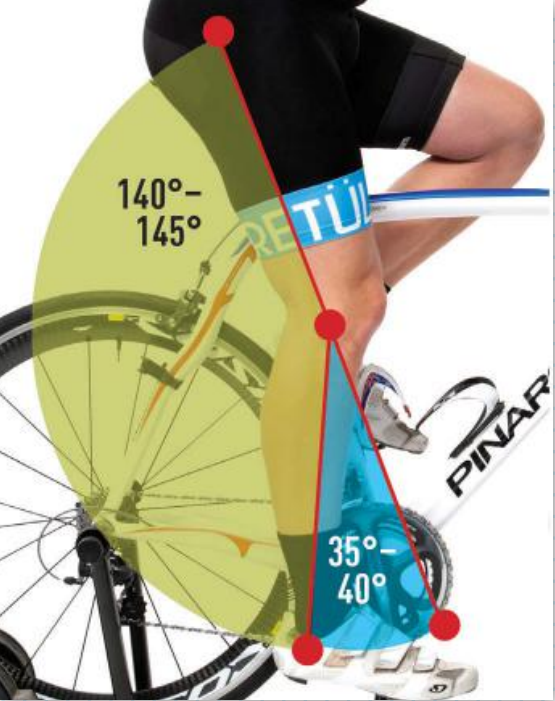
\includegraphics[width=0.5\textwidth]{obrazky-figures/burt_knee_angle.png}
    \caption{Knee extension angle of 140-145 degrees, which is often referred to as 35-40 degrees (being the angle of deviation from straight leg). Is considered optimal for the average rider. Taken from \cite{burtbikefit}.}
    \label{fig:saddle_height}
\end{figure}



Higher saddle height can help to better recruitment of glutens and hamstrings, which can lead to more power output. However, it requires more flexibility and can lead to injury if the rider is not flexible enough. Similarly too low saddle height can increase the compressive forces on the knee and lead to pain and injury.

Proper saddle height is therefore a balance between power output and comfort. It is also important to note that the saddle height is not the only factor that affects the knee angle. The saddle fore and aft position and the cleat position also affect the knee angle.

\subsection{Saddle Setback}
Saddle setback or saddle fore and aft position refers to the horizontal position of the saddle with respect to the bottom bracket.

% \begin{figure}
%     \centering
%     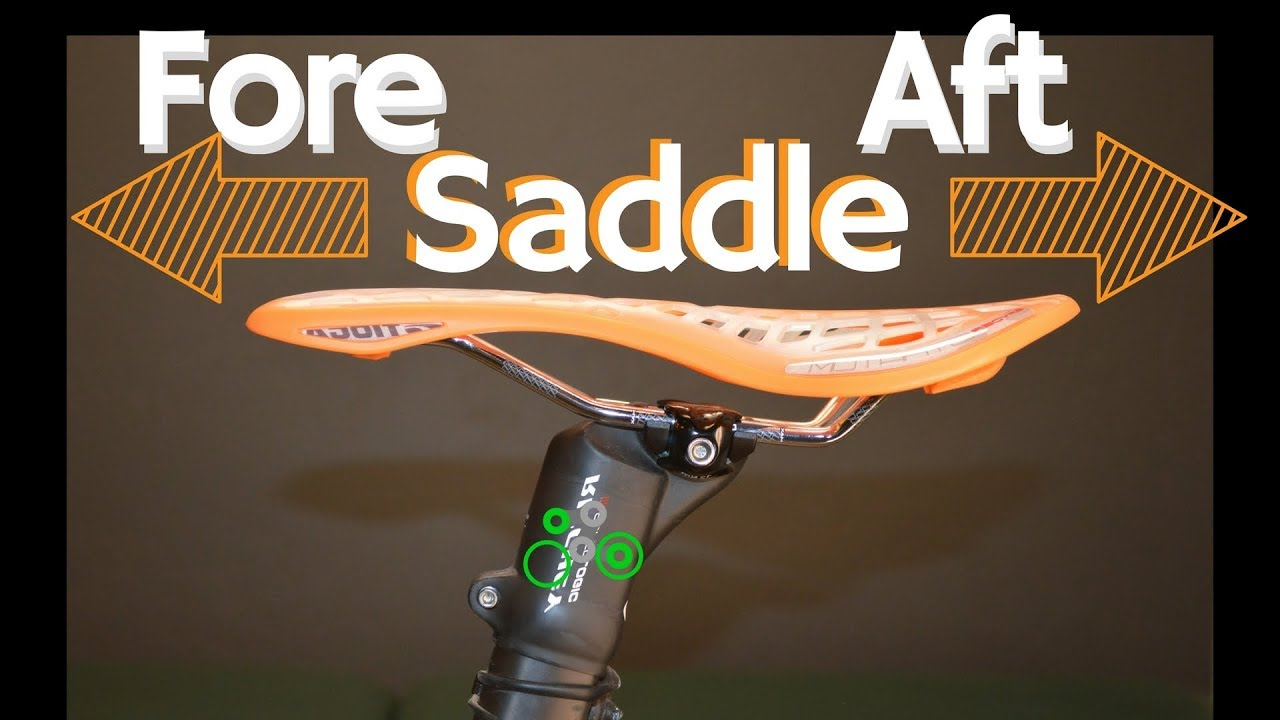
\includegraphics[width=0.8\textwidth]{obrazky-figures/saddle_fore_aft.jpg}
%     \caption{Saddle setback is adjusted by sliding the saddle saddle rails forward or backward in the seatpost clamp. Taken from Bike Fit Adviser's \href{https://www.youtube.com/watch?app=desktop&v=SZhWVZq2qUc}{video} on saddle setback.}
%     \label{fig:saddle_fore_aft}
% \end{figure}

Setback is most often measured at the 3 o'clock position of the crank. At this position, the rider's knee should be directly above the pedal spindle. Having the knee too far back it is harder to generate power. Having the knee too far forward can lead to knee pain due to increased forces on the kneecap \cite{burtbikefit}.

Saddle setback also affects the rider's balance on the bike. Having the saddle too far forward can lead to the rider's weight being too far forward, which can lead to hand pain because of too much weight on the handlebars. Having the saddle too far back can lead to the rider's weight being too far back, which can lead to make the front wheel feel light and make the bike harder to control.

Setback also affects the rider's hip angle. Hip angle is the angle between the shoulder and the knee measured at the hip. Having the saddle more forward can lead to a more open hip angle, which can lead to more power output and more space between the rider's torso and legs at the top of the pedal stroke. This is why time trial bikes have a more forward saddle position.



\subsection{Handlebar Height and Reach}
Handlebar height measures how high the handlebars are in relation to the saddle. Handlebar reach measures how far the handlebars are in relation to the saddle.

Handlebar height influences mainly torso angle and to and also shoulder angle. Torso angle is the angle between the shoulder and the level plane measured at the hip. It is also known as the back angle. Shoulder angle is the angle between the hip and wrist measured at the shoulder. Handlebar reach influences mainly shoulder angle.

Handlebar height can be adjusted by changing the number of spacers under the stem or by changing the stem itself. Handlebar reach can be adjusted by changing the stem length or by changing the handlebars themselves.

While optimal handlebar height and reach are highly individual, there are some general guidelines. For example, a more upright position is more comfortable and is therefore recommended for longer rides. A more aggressive position is more aerodynamic and is therefore recommended for racing. Burt recommends back angle of about 45 degrees for average riders and shoulder angle of about 90 degrees with the elbow slightly bent \cite{burtbikefit}. For faster riders, the back angle can be lowered down to 30 degrees with more open shoulder angle. For more upright riders, the back angle can be increased up to 55 degrees with more closed shoulder angle.


%%%%%%%%%%%%%%%%%%%%%%%%

\section{Existing Solutions for Automated Bikefitting}

\subsection{MyVeloFit}
\href{https://www.myvelofit.com/}{MyVeloFit}  is a web application that uses pose estimation model to predict the joint locations for a side view video of the user pedaling their bike on an indoor trainer. Based on location of these joints, joint angles are then computed. On the basis of these angles and their relation to average angles, suggestions are made for adjusting the position of the saddle and handlebars.

The fitting process starts with the rider filling out questionaire about their mobility. This is then used to adjust the recommended angle ranges. For example: if the user has lower shoulder mobility, recommended ranges for shoulder angle will be increased so the user is not stretched forward so much.

After creating the user profile, user can create a fit session for one specific bike. In the process, the user selects their fit goal (performance, comfort, or balanced) and the type of bike they are using (road, gravel, mtb, triathlon, hybrid, or stationary). This also changes the recommended angle ranges.

\subsubsection{Predicted keypoints}
MyVeloFit predicts 6 joint locations for the camera facing side of the body. Most common pose estimation models predict similar keypoints. However, keypoints commonly used to adjust the position of the saddle, such as the heel and the fifth metatarsal of the foot, are missing. The keypoints used by MyVeloFit are: ankle, knee, hip, shoulder, elbow and wrist. Figure \ref{fig:myvelofit_keypoints} shows the predicted keypoints.


\begin{figure}[htbp]
    \centering
    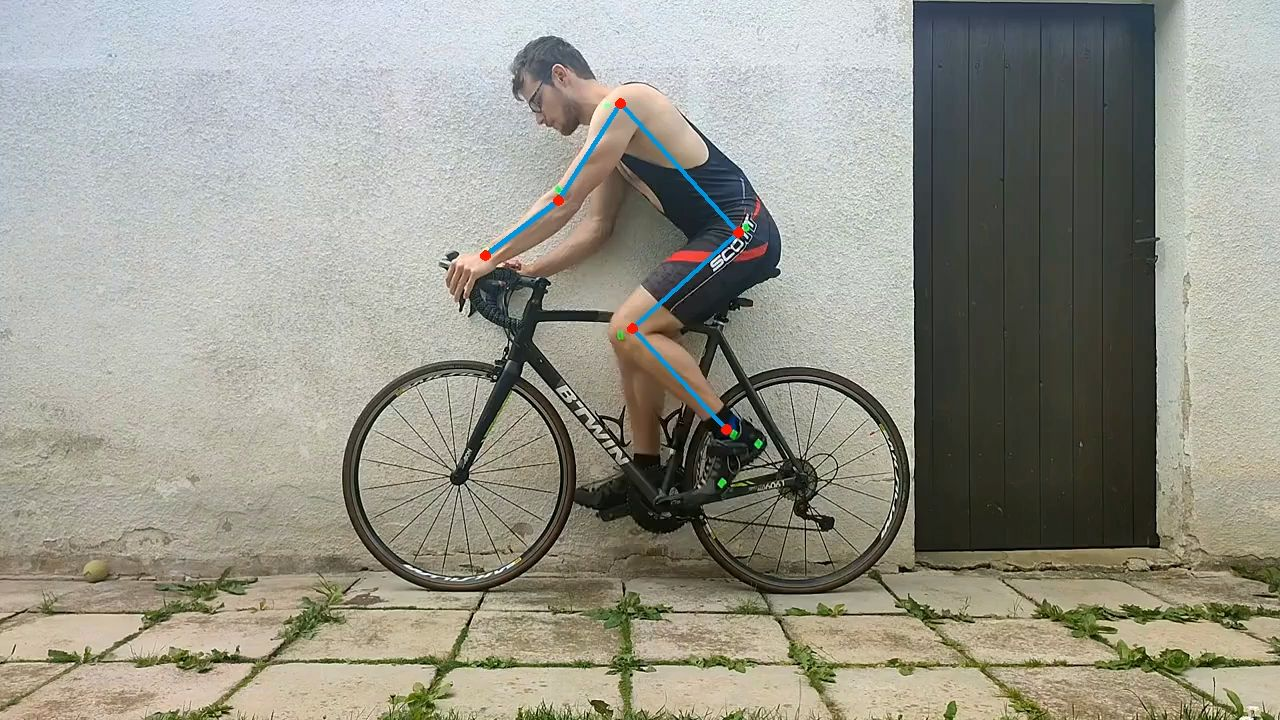
\includegraphics[width=\textwidth]{obrazky-figures/myvelofit_keypoints.jpg}
    \caption{Side view image with predicted keypoints in MyVeloFit.}
    \label{fig:myvelofit_keypoints}
\end{figure}

From the joint angles for every frame, some are selected for computing the joint angles at the top of the pedal stroke, front of the pedal stroke and bottom. Every position uses different angle ranges and even which angles are taken into account. Figure \ref{fig:myvelofit_top} shows the predicted joint angles at the top of the pedal stroke.

\begin{figure}[htbp]
    \centering
    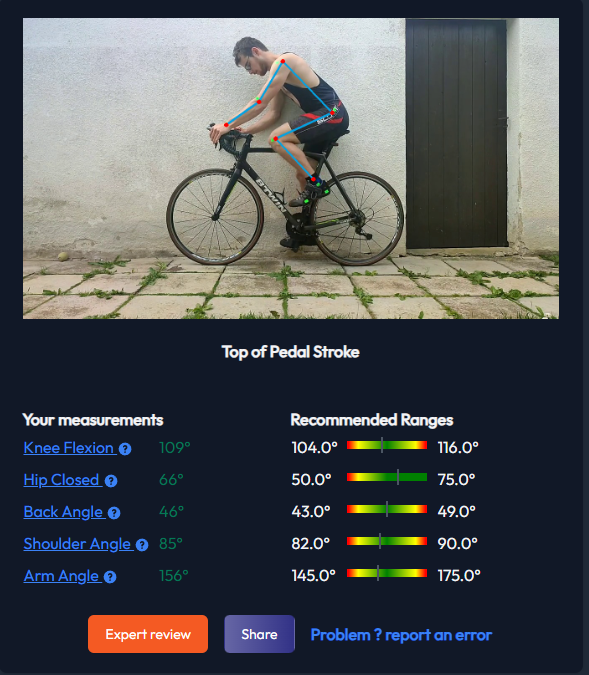
\includegraphics[width=0.6\textwidth]{obrazky-figures/myvelofit_top.png}
    \caption{Predicted joint angles at the top of the pedal stroke in MyVeloFit.}
    \label{fig:myvelofit_top}
\end{figure}

Based on the angles computed for parts of the pedal stroke, MyVeloFit then makes suggestions for saddle height, saddle fore and aft, handlebar height and handlebar reach. Figure \ref{fig:myvelofit_suggestions} shows the recommended changes to the bike position.

\begin{figure}[htbp]
    \centering
    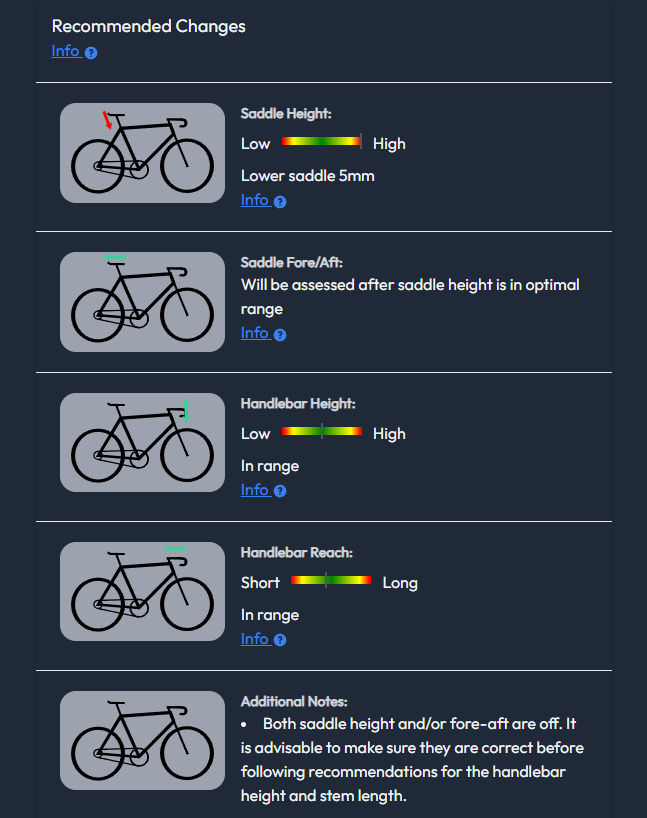
\includegraphics[width=0.6\textwidth]{obrazky-figures/myvelofit_suggestions.png}
    \caption{Recommended changes to the bike position based on the angles computed by MyVeloFit.}
    \label{fig:myvelofit_suggestions}
\end{figure}

Overall, MyVeloFit is relatively easy to use and its joint predictions are fairly accurate. However, it has few disadvantages:

\begin{itemize}
    \item Only the most basic keypoints are used.
    \item Every video is converted to 30 FPS and cut down to 10 seconds.
    \item Video processing and keypoint predictions are slow (3-5 minutes).
    \item Requires subscription to get joint angles and recommended changes. Either a one time payment of 35 US dollars for access for 1 person and 1 bike for 2 weeks or 75 US dollars annually for unlimited number of bikes and people.
\end{itemize}


\subsection{Retül}
\href{https://www.retul.com/}{Retül} is a bike fitting system employing 3D motion capture technologys. It utilizes infrared LED markers placed on specific body points to track the rider's movements dynamically while cycling. The led markers are tracked by multiple infrared cameras placed around the rider. The cameras surprisingly capture only 18 frames per second. Despite this research \cite{retulReliability} shows that the system is relatively reliable compared to 3d motion capture systems with higher frame rates.

Retül uses 8 markers placed on both sides of the rider's body. These markers are placed on the following locations: fifth metatarsal of the foot, heel, ankle, knee, hip, shoulder, elbow and wrist.


The markers are placed by the fitter on the rider's body. Accurate placement of the markers is crucial for the system to work properly. Even small deviations can lead to inaccurate results. Figure \ref{fig:retul_markers} shows the placement of the markers.

\begin{figure}[htbp]
    \centering
    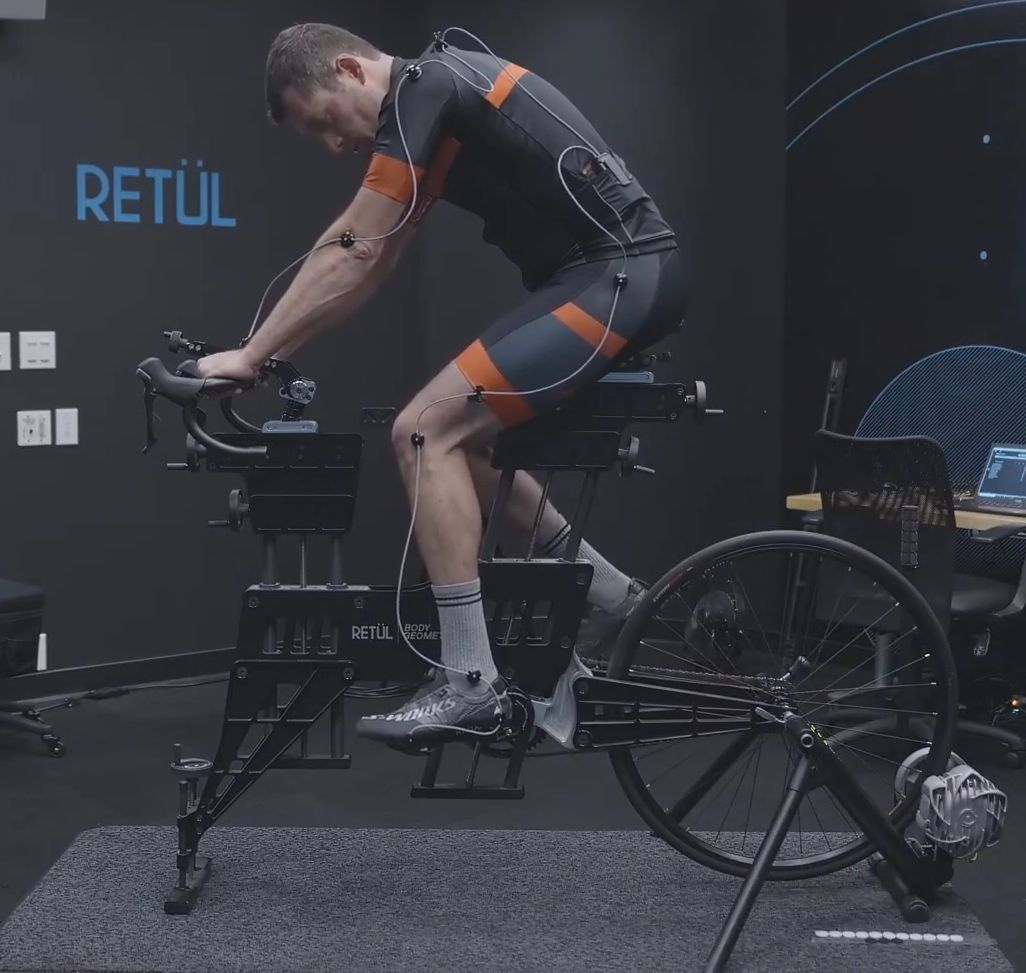
\includegraphics[width=\textwidth]{obrazky-figures/retul_markers.jpg}
    \caption{Placement of the markers used by Retül. (Screenshot from instructional instructional video by Retül \cite{retulMarkersYoutube}.)}
    \label{fig:retul_markers}
\end{figure}

Retül's fitting process involves setting up the bike on a trainer equipped with the system. During the session, the rider performs various motions and pedal strokes while the Retül system captures real-time data on joint angles and movements.

Data Captured by Retül includes a wide range of joint angles and movements such as knee angles at top of the pedal stroke and bottom of the pedal stroke, hip angles throughout the pedal stroke, shoulder, elbow, and wrist positions in relation to handlebar reach and drop, as well as ankle and foot movement concerning cleat positioning and alignment. Figure \ref{fig:retul_app} shows the captured data in Retül's software.

\begin{figure}[htbp]
    \centering
    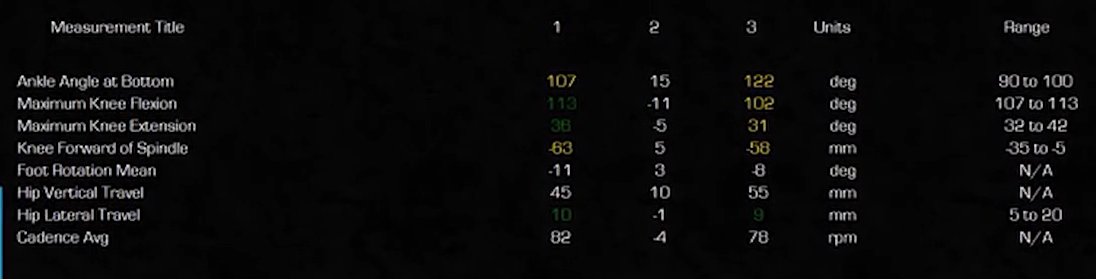
\includegraphics[width=\textwidth]{obrazky-figures/retul_app_crop.png}
    \caption{Retül's software showing the captured data. (Screenshot from  instructional video by Retül \cite{retulScreenYoutube}.)}
    \label{fig:retul_app}
\end{figure}

The normal ranges for these angles were constructed based on the data collected from thousands cyclists. However, these cyclists were not necessarily optimally fitted to their bikes. Therefore, the normal ranges may not be based on the optimal position for the rider.

Based on the captured data, Retül compares the rider's position to the normal ranges. Based on this comparison, the fitter can make changes to the bike position.

Despite the fact that Retül is a very popular bike fitting system, it has some important disadvantages:
\begin{itemize}
    \item Costly equipment and setup requirements, limiting accessibility to some individuals or smaller bike shops.
    \item The need for trained Retül bike fitters to interpret and implement fitting recommendations effectively.
    \item Requires in-person fitting sessions. These sessions can be time-consuming and costly.
\end{itemize}


\subsection{BikeFast Fit Elite}
\href{https://www.bikefastfit.com/}{BikeFast Fit Elite} is an iOS and Mac OS application that uses pose estimation model to predict the joint locations for a side view video of the user pedaling their bike on an indoor trainer. Compared to MyVeloFit, it uses additional keypoints for the fifth metatarsal of the foot and the heel. Figure \ref{fig:bikefastfit_keypoints} shows the predicted keypoints.

\begin{figure}[htbp]
    \centering
    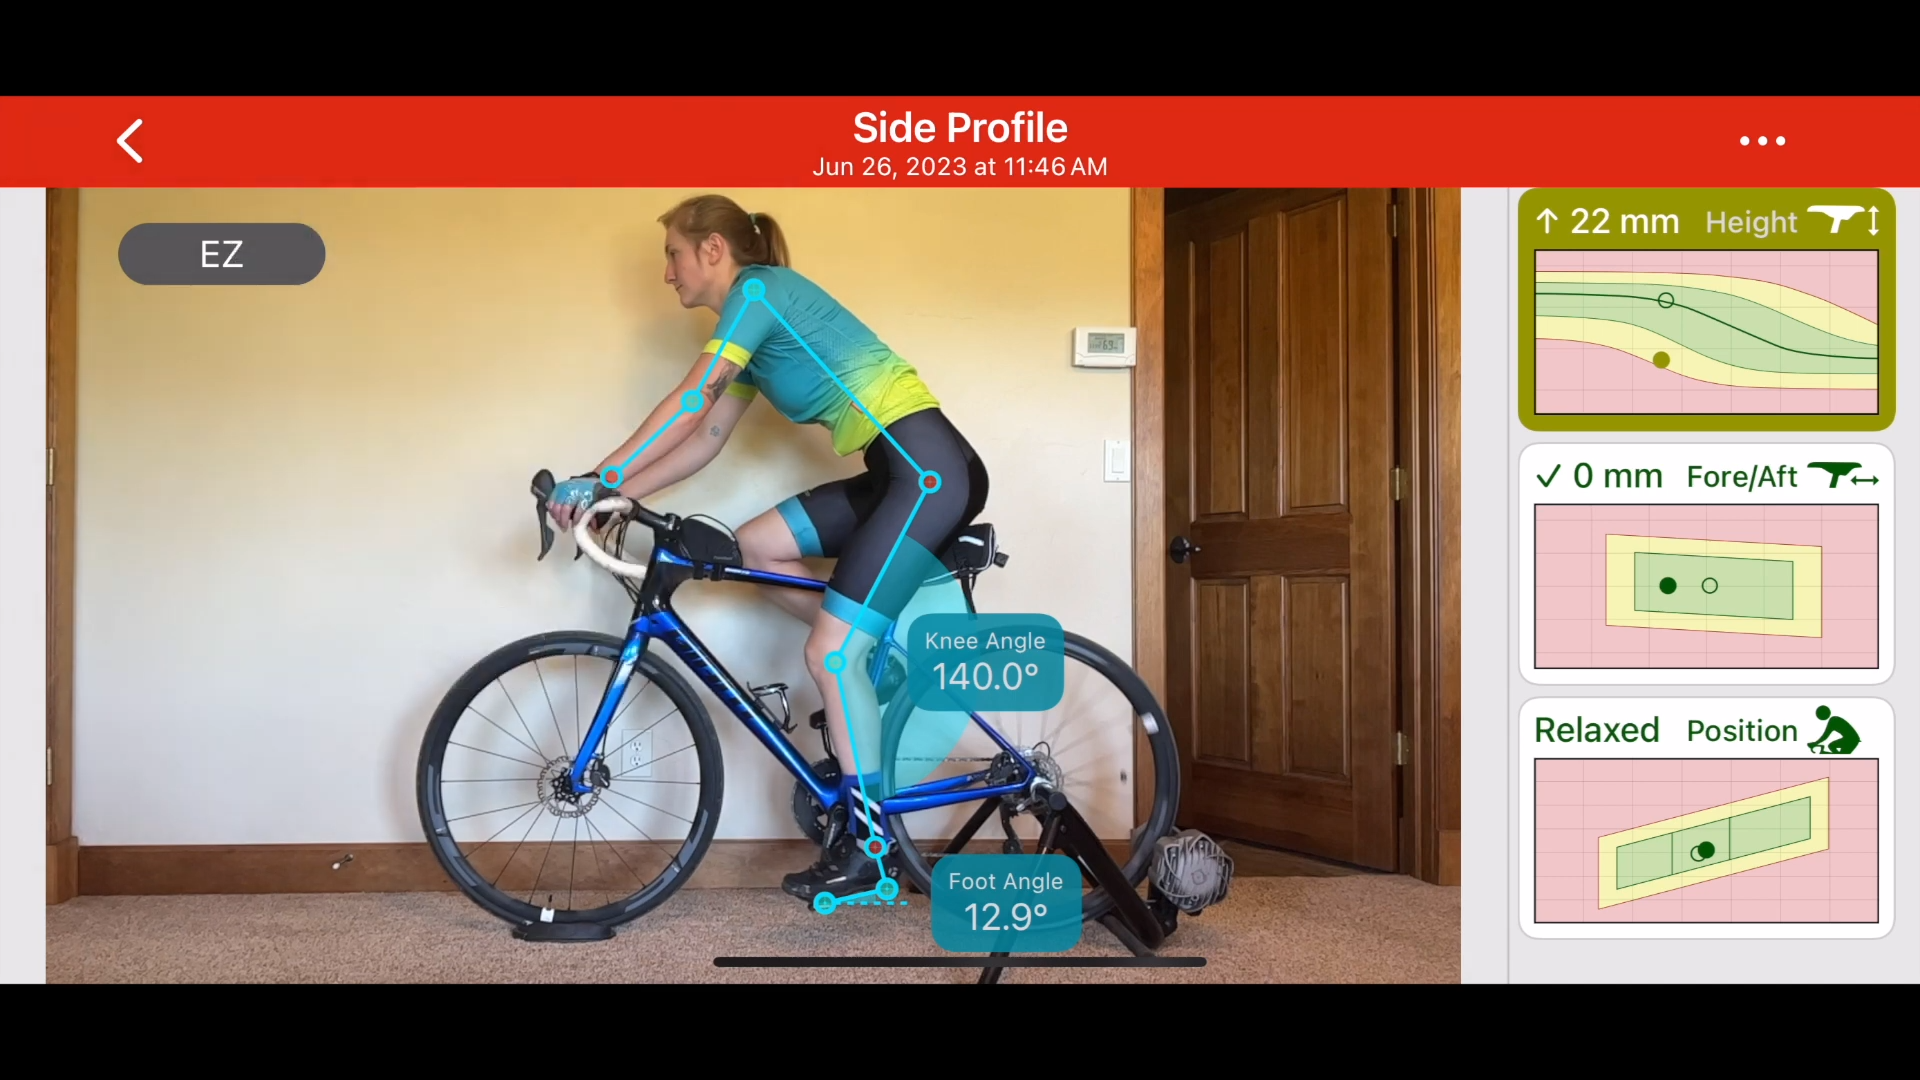
\includegraphics[width=\textwidth]{obrazky-figures/bike_fast_fit_elite.png}
    \caption{Side view image with predicted keypoints in BikeFast Fit Elite. (Screenshot from promotional video \cite{bikeFastFitElitev2Youtube} by BikeFast Fit Elite.)}
    \label{fig:bikefastfit_keypoints}
\end{figure}

Similarly to MyVeloFit, it suggest changes to the saddle height and fore and aft position but it does not suggest changes to the handlebar position, arguing that the handlebar position is based on individual goals and flexibility.

Additionally, it also provides front view knee tracking to address possible knee wobble and asymmetry.

% TODO: rozepsat

The app costs 19.99 US dollars and does not require a subscription. However, it is only available for iOS and Mac OS. Also it only captures 3.5 seconds of video.


\chapter{Marker-based Tracking}
\label{marker_based_tracking}
To automatically fit a bike to a rider, a bikefitting system needs to estimate the rider's pose. One way to estimate the cyclist's pose is to use colored markers, which are placed on the parts of the body. These markers can then be accurately detected and tracked in the video. The position of the markers can then be used to estimate the keypoints of the rider's body.

This chapter describes an approach to estimating the keypoints of the rider's body using colored markers and color thresholding. The markers are first manually localized by the user in the first frame of the video. The color of the markers is then used to detect them in the following frames. The markers are then tracked using a method similar to SORT \cite{sort}.

Following sections describe the implementation of this approach in OpenCV.js \cite{opencvjs} and discusses its advantages and limitations.

\section{Localization and Tracking Pipeline}

\subsection{Manual Localization of the Markers}
\label{manual_localization_of_the_markers}
At first, the user is asked to manually localize the markers by clicking on them in the first frame of the video. Figure \ref{fig:marker_localization} shows an example of the manual localization of the markers. The colors of these markers are saved and used for thresholding and detection of the markers in the following frames. The user is asked to first localize the marker on the foot, then the marker on the heel, then the marker on the ankle, etc. Figure \ref{fig:marker_localization} shows the manual localization process of the markers.

\begin{figure}[htbp]
    \centering
    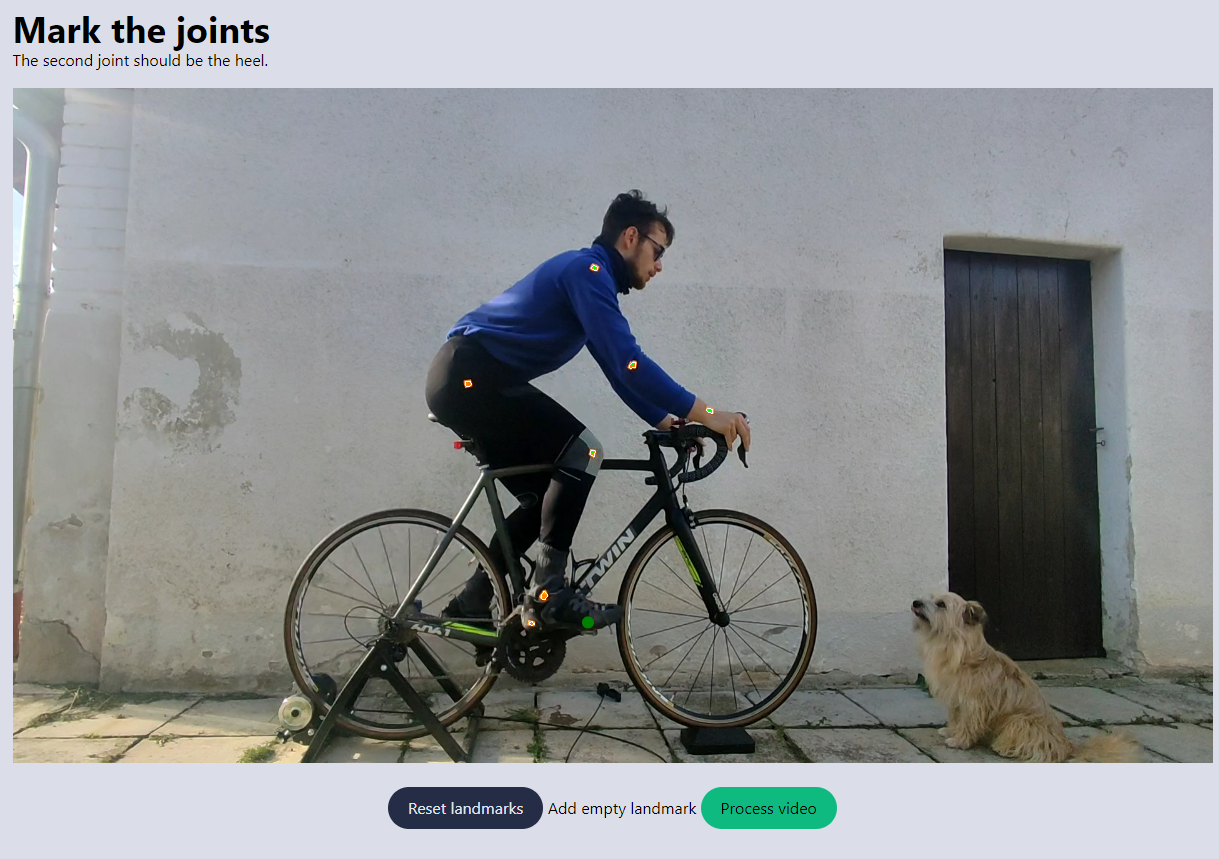
\includegraphics[width=\textwidth]{obrazky-figures/markers_localization.png}
    \caption{Example of the manual localization of the markers. The user is asked to click on the markers in the first frame of the video. The single localized foot marker is highlighted in green.}
    \label{fig:marker_localization}
\end{figure}




After clicking on a marker, multiple steps are performed:
\begin{enumerate}
    \item The x,y coordinates of the marker are saved.
    \item If there is already some marker localized and therefore some color thresholds defined and markers detected, the detected markers are searched if there is some marker close to the clicked marker. If there is, the location of the clicked marker is updated to the location of the detected marker. This is done so that user does not have to precisely click on the marker. This is especially useful when the markers are small and the user is using a mobile device with a small screen.
    \item Based on the x,y coordinates of the marker, the color of the marker is extracted from the image.
    \item The color of the marker is used to update the color thresholds used to detect the markers. More on this in section \ref{detection}.
\end{enumerate}

Figure \ref{fig:marker_crop} shows a closeup of the localization of the markers. The single localized foot marker is highlighted in green. The contours of the thresholded regions are highlighted in white. The centroids of the contours are highlighted by small green cross.
\begin{figure}[htbp]
    \centering
    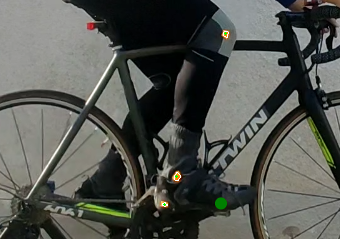
\includegraphics[width=\textwidth]{obrazky-figures/markers_crop.png}
    \caption{Closeup of the localization of the markers. The single localized foot marker is highlighted in green. The contours of the thresholded regions are highlighted in white. The centroids of the contours are highlighted by small green cross.}
    \label{fig:marker_crop}
\end{figure}

\subsection{Detection}
\label{detection}
After obtaining the markers locations and colors, the markers are detected in the following frames. The detection is performed in the following steps:
\begin{enumerate}
    \item The frame is converted to the CIELAB color space.
    \item The frame is thresholded using the minimum and maximum A and B channel values of the localized markers and some margin. The margin is used to account for the changes in the lighting conditions. Empirically, the margin of 15 works well. Figure \ref{fig:marker_detection} shows an example of the thresholded image.
    \item Contours are found in the thresholded image. The \texttt{cv.findContours()} method is used for this.
    \item The centroids of the contours are calculated using the \texttt{cv.moments()} method.
    \item The centroids are used as noisy detections.
\end{enumerate}

The CIELAB color space is used because it is designed to approximate human vision. The A and B channels are used because they represent the color of the marker. The L channel is not used because it represents the lightness of the color and is not very useful for detecting the markers due to the changes in the lighting conditions. Experiments with using the H channel of the HSV color space were also performed, but there were some problems with the detection of the markers on the edges of the color spectrum (H=0 and H=255). The CIELAB color space does not have this problem, because it uses two channels for the color. Figure \ref{fig:marker_detection} shows an example of the thresholded image.

\begin{figure}[htbp]
    \centering
    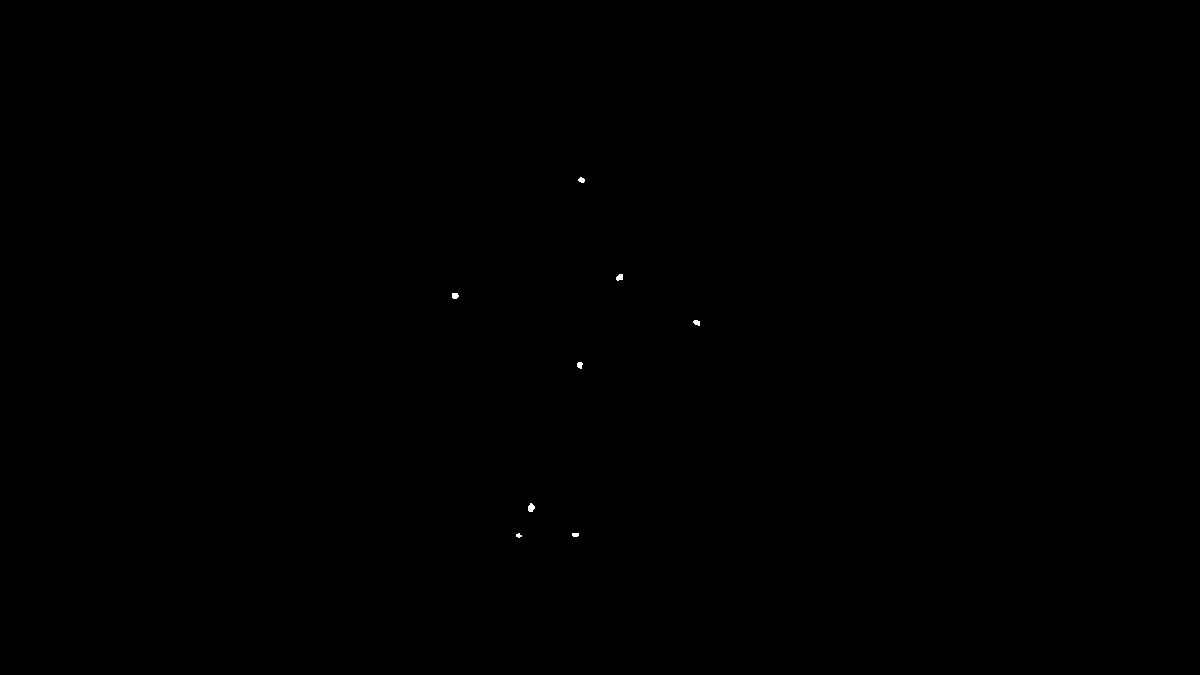
\includegraphics[width=\textwidth]{obrazky-figures/thresholded.png}
    \caption{Example of the image thresholded using the minimum and maximum A and B channel values of the localized markers and a margin of 15. The markers are then detected as the centroids of the contours in the thresholded image.}
    \label{fig:marker_detection}
\end{figure}

\subsection{Tracking}
\label{tracking}
The detected markers are then tracked using a simple method similar to SORT \cite{sort}. The tracking algorithm works as follows:

\begin{enumerate}
    \item Every possible assignment of the detected markers and the markers in the previous frame is created. To limit the number of possible assignments, the assignments are created only if the distance between the markers is less than 50 pixels.
    \item For every found assignment, the cost of the assignment is calculated as the sum of the distances between the markers in the assignment.
    \item To make tracking more robust, the cost of the assignment is increased by the difference of the angles between the markers in the assignment. This is done to prevent the markers from switching places.
    \item Assignment with the most markers assigned and the lowest cost is selected.
\end{enumerate}

Experiments with using the Kalman filter were also performed, unfortunately the author was not able to get the Kalman filter to work properly.

\section{Advantages and Limitations}
The marker-based approach was mainly chosen due to its theoretically perfect accuracy, which is
its biggest advantage. However, in practice there are several limitations to this approach:

\begin{enumerate}
    \item Accuracy of the system heavily depends on the placement of the markers. If the markers are not placed correctly, the results are not accurate. Since the placement is done by the user, this is a real issue. Correct placement of the markers is not trivial.
    \item The user needs to have the markers available. They don't have to be special video markers, but they need to be of a different color than the background and the clothing of the user and need to be glued to the user.
    \item The biggest limitation is the reduced robustness of the system. The system works well if the color of the markers is not present elsewhere in the image. However, in other cases, the markers are detected in the wrong places and the system does not work. Figure \ref{fig:failed_localization} shows an example of the failed localization of the markers. The knee marker is not localized correctly, because the leaves in the background have similar color to the markers.
\end{enumerate}

\begin{figure}[htbp]
    \centering
    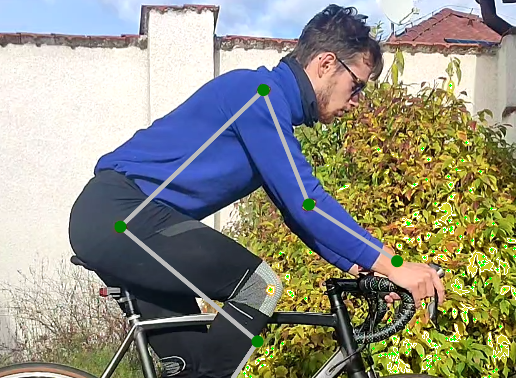
\includegraphics[width=\textwidth]{obrazky-figures/failed_localization_crop.png}
    \caption{Example of a failed localization of the markers. The leaves in the background have similar color to the markers and the knee marker is therefore not localized correctly. The location of the markers is show as the green dots.}
    \label{fig:failed_localization}
\end{figure}

Due to these serious limitations, the marker-based approach was not used in the final version of the application. And instead, the RTMPose pose estimation model is used. The details of the implementation are described in section \ref{pose_estimation}.



%%%%%%%%%%%%%%%%%%%%%%%%%%%%%%%%%%%%%

\chapter{Pose Estimation Models}
\label{ch:pose_estimation}

This chapter describes some of the good performing pose estimation algorithms and compares their performance on the task of side view pose estimation of cyclists.

Pose estimation is a computer vision task that involves predicting the locations of keypoints on a person in an image or a video. The keypoints are usually the joints of the person, such as the ankle, knee, hip, shoulder, elbow, wrist, etc. The pose estimation models are usually trained on datasets that contain images or videos with annotated keypoints. The models are then evaluated on the same datasets.

There are multiple approaches to pose estimation. The most common approaches are the top-down approach and the bottom-up approach. The top-down approach first detects people in the image and then predicts the keypoints for each person. The bottom-up approach first predicts the keypoints and then groups them into poses using hand writte post processing algorithms. Another approach is the one-stage approach, which predicts the keypoints directly from the image without the need for post processing. This work evaluates three pose estimation models using the top-down approach (RTMPose, HRNet and ViPNAS), described in sections \ref{rtmpose}, \ref{hrnet} and \ref{vipnas} and one pose estimation model using the one-stage approach (YOLOX-Pose), described in section \ref{yolox-pose}.

Not all of the models predict the same keypoints. The models predict either 17 keypoints, as defined in the COCO dataset \cite{coco}, 26 keypoints, as defined in the Halpe26 dataset \cite{halpe}, or 133 keypoints, as defined in the COCO-WholeBody dataset \cite{coco-wholebody}. Figure \ref{fig:subfigures} shows the sets of keypoints used by the MS-COCO dataset, the Halpe26 dataset and the COCO-WholeBody dataset.

\begin{figure}[htbp]
    \centering
    \begin{subfigure}[b]{0.2\textwidth}
        \centering

        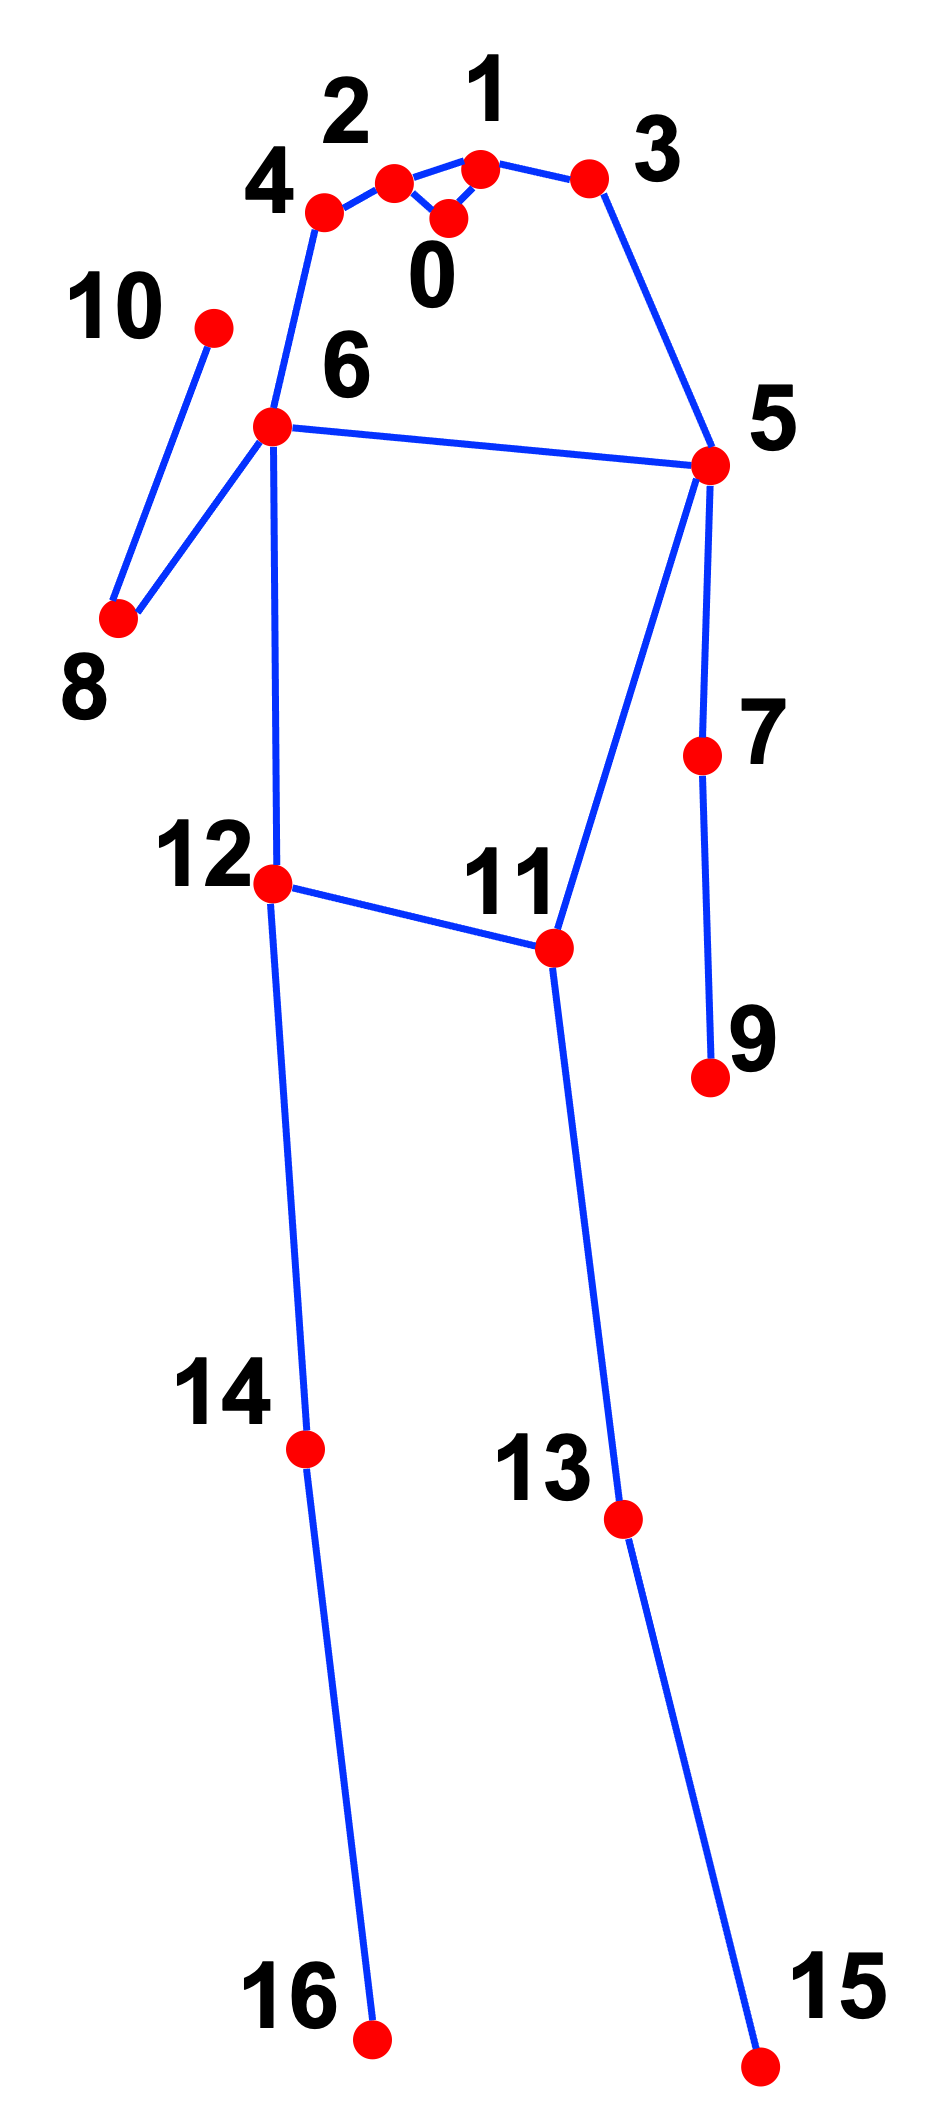
\includegraphics[height=8cm]{obrazky-figures/coco_landmarks.png}
        % \caption{MS-COCO keypoints. Taken from \cite{coco}.}
        \label{fig:image1}
    \end{subfigure}
    \hfill
    \begin{subfigure}[b]{0.25\textwidth}
        \centering

        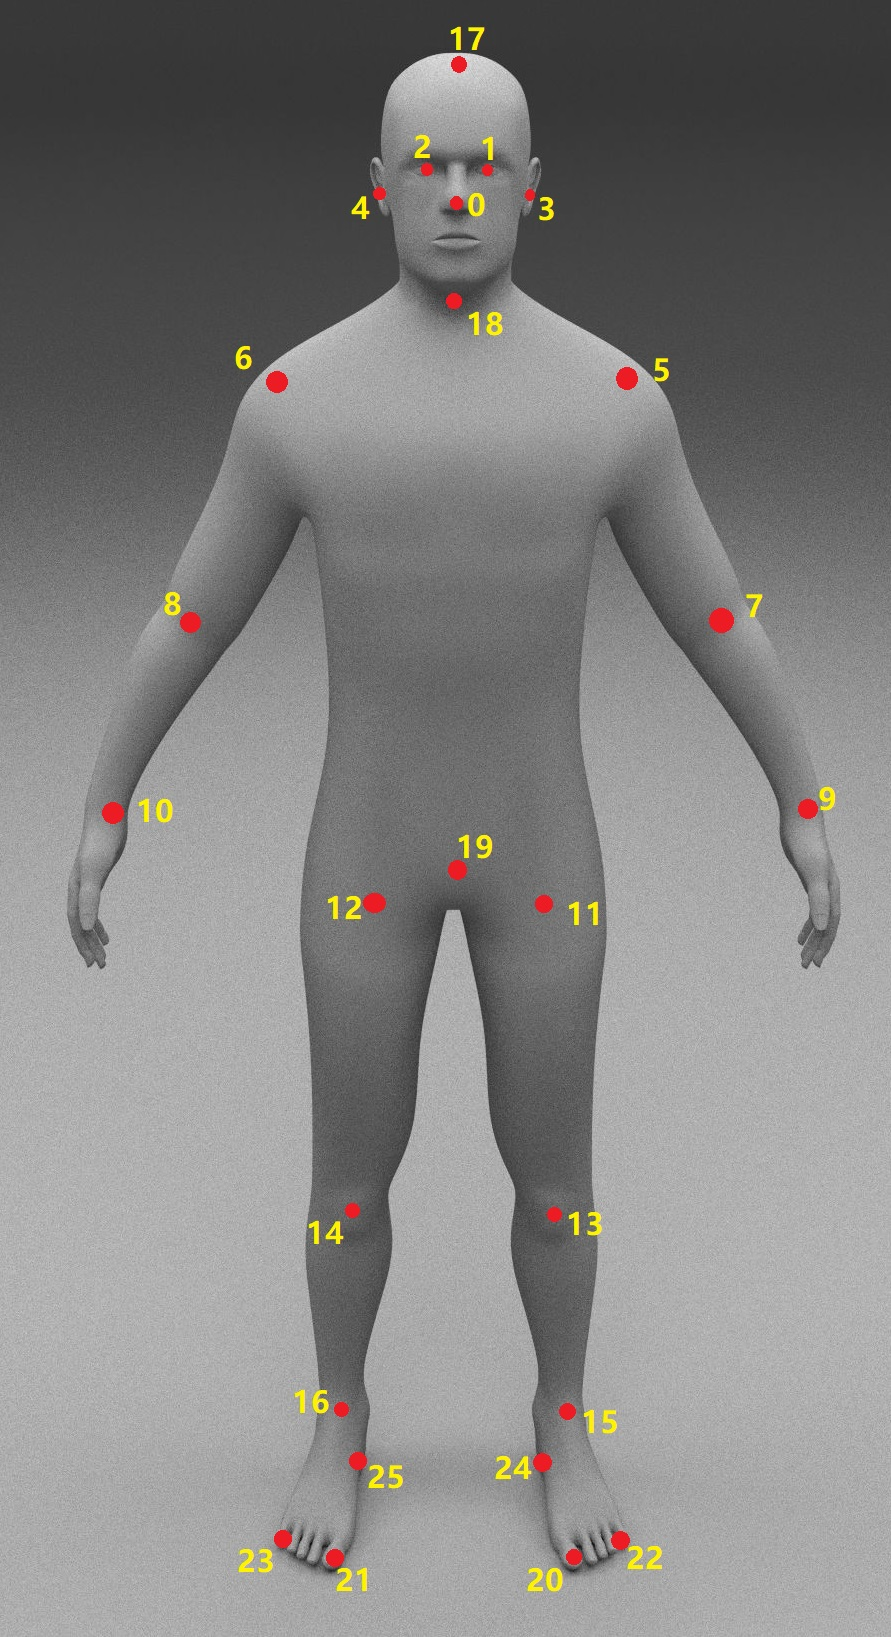
\includegraphics[height=8cm]{obrazky-figures/halpe_landmarks.jpg}
        % \caption{Halpe26 keypoints. Taken from \cite{halpe}.}
        \label{fig:image2}
    \end{subfigure}
    \hfill
    \begin{subfigure}[b]{0.5\textwidth}
        \centering

        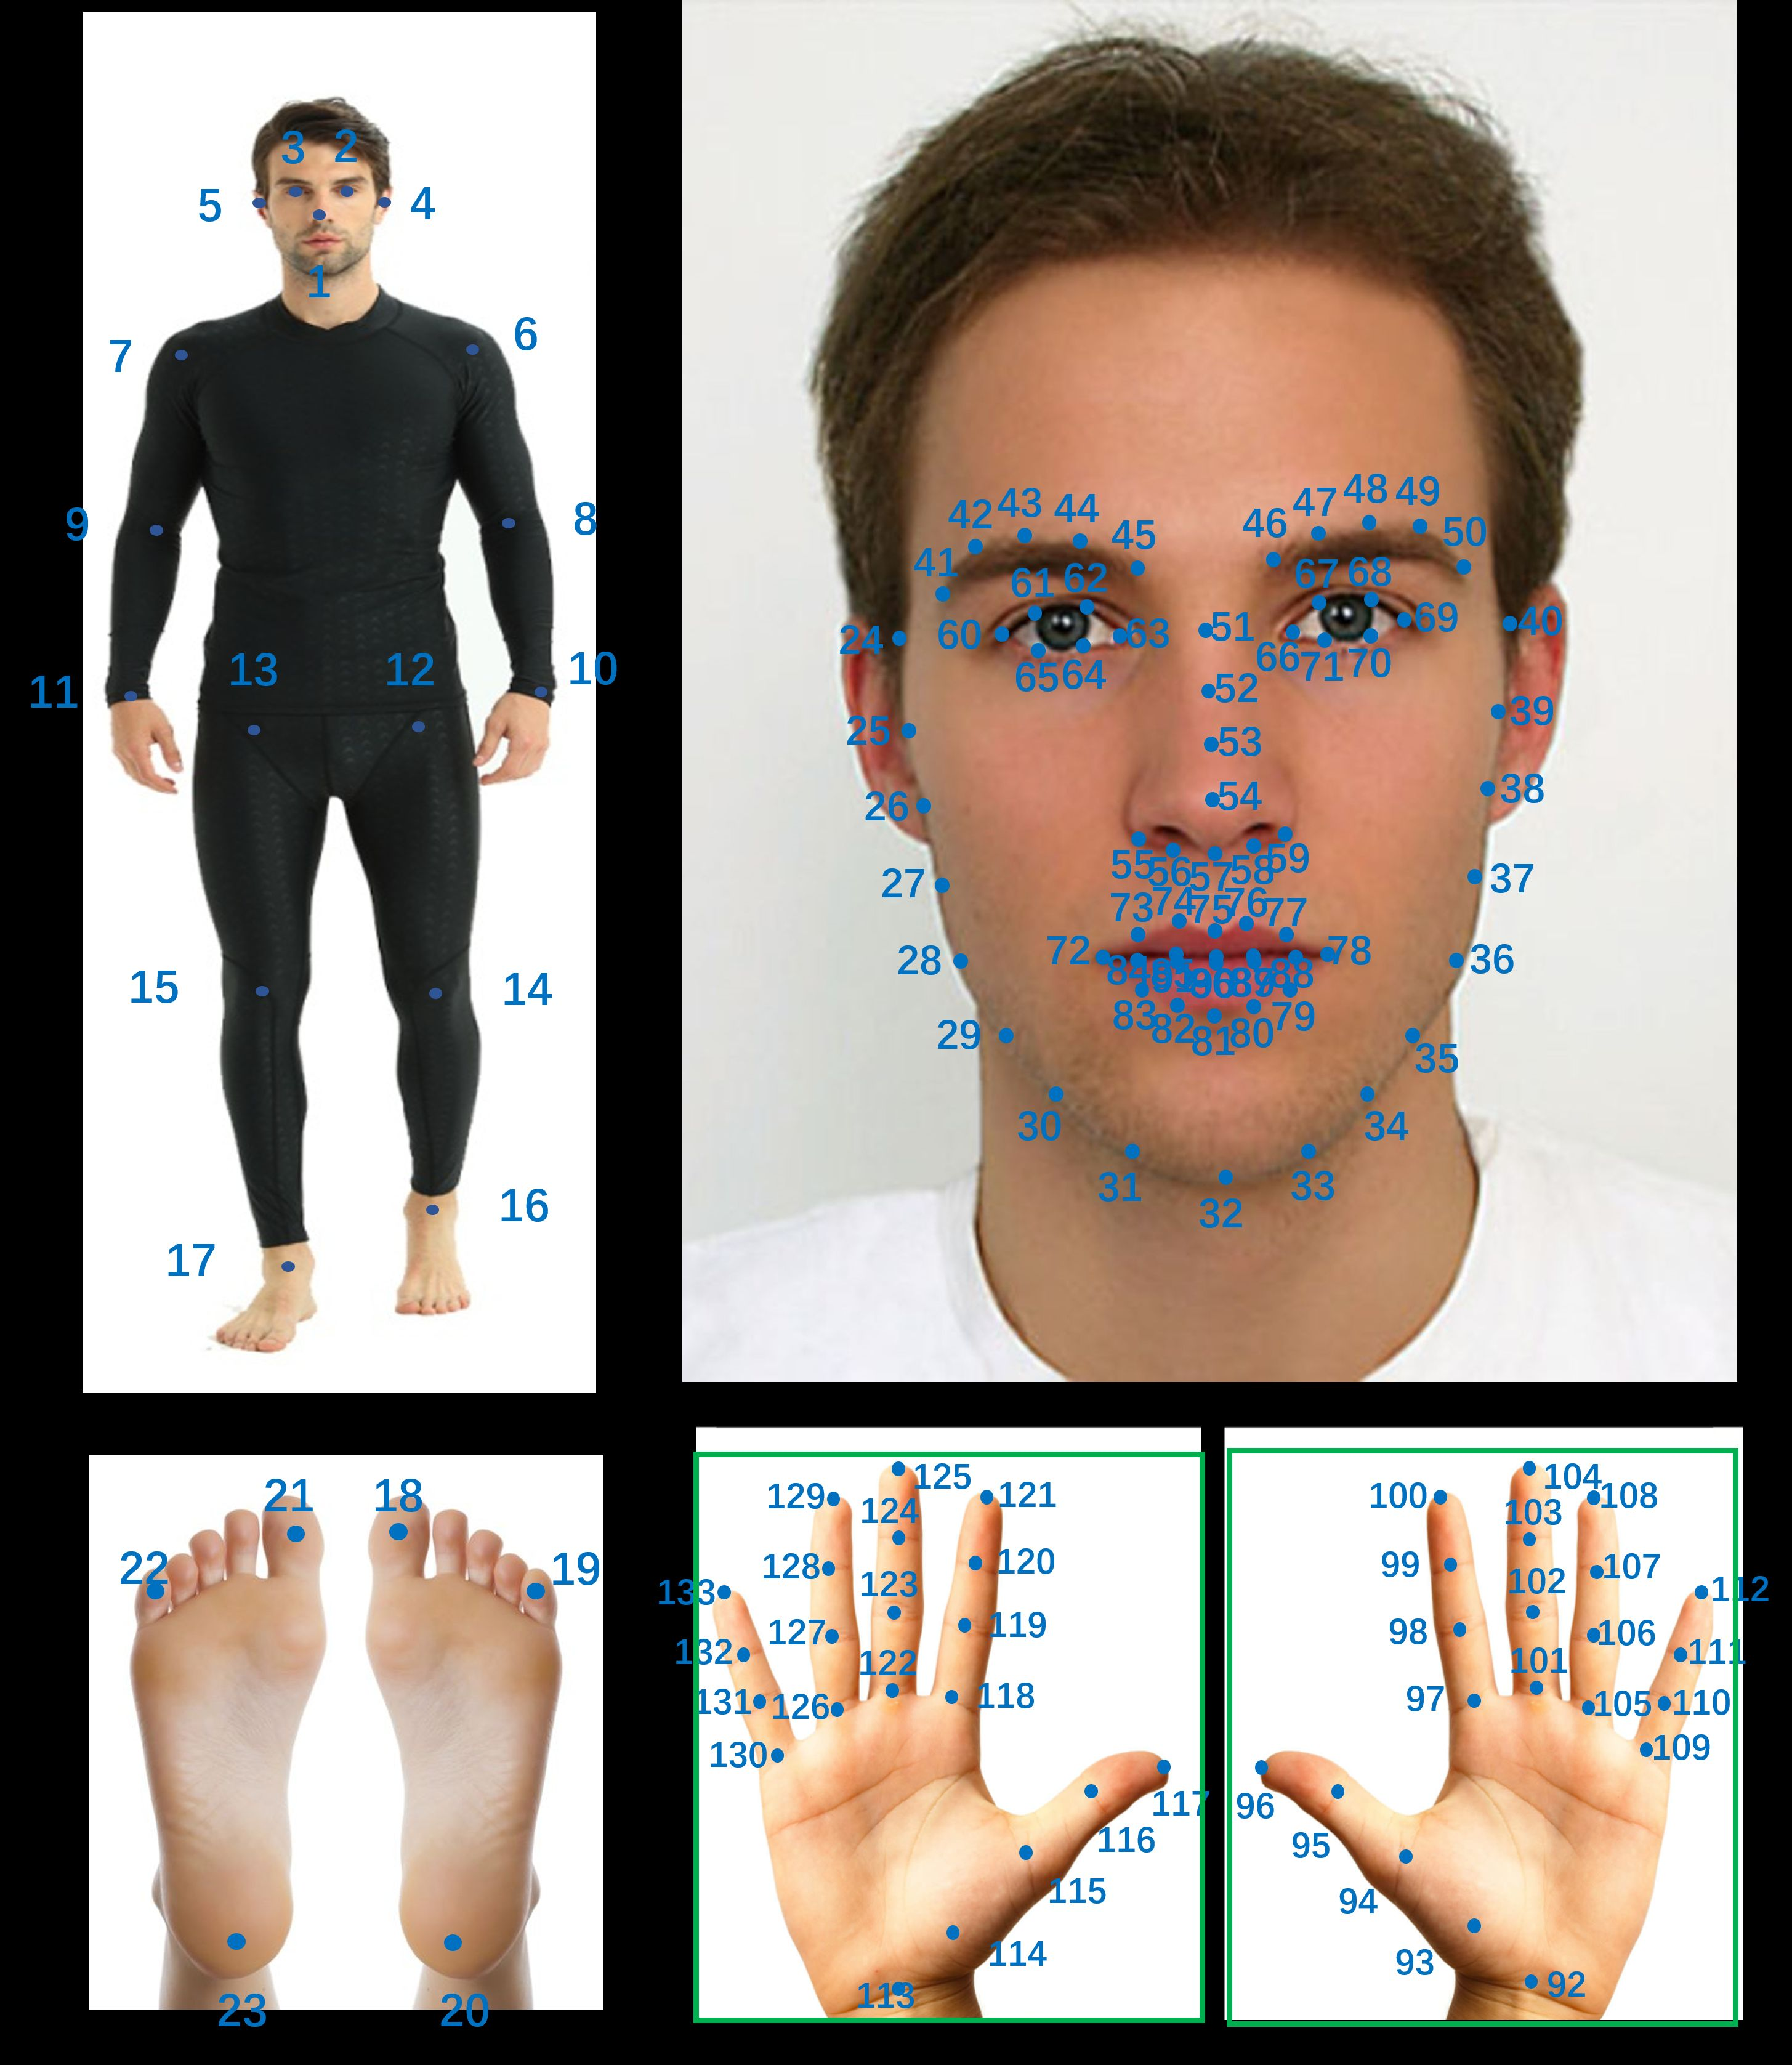
\includegraphics[height=8cm]{obrazky-figures/coco_wholebody_landmarks.jpg}
        % \caption{COCO-WholeBody keypoints. Taken from \cite{coco-wholebody}.}
        \label{fig:image3}
    \end{subfigure}

    \caption{Sets of keypoints used by (from left to right) MS-COCO dataset, Halpe26 dataset and COCO-WholeBody dataset (images taken from \cite{coco} and \cite{halpe}).}
    \label{fig:subfigures}
\end{figure}



\section{RTMPose}
\label{rtmpose}

RTMPose \cite{rtmpose} is a pose estimation model from the authors of the MMPose framework \cite{mmpose2020}. It is designed to bridge the gap between the excellent performance of 2D pose estimation on public benchmarks and its application in the industrial community, which still suffers from heavy models and high latency.

The RTMPose models are designed to be lightweight and fast. The authors claim, that the RTMPose-m achieves 75.8\% AP on COCO with 90+ FPS on an Intel i7-11700 CPU and 430+ FPS on an NVIDIA GTX 1660 Ti GPU. The RTMPose-s model, achieving 72.2\% AP on COCO was also tested on a mobile device with the Snapdragon 865 chip, running at 70+ FPS.

\subsection{Architecture}

The RTMPose models are based on the top-down pose estimation approach. They use a two-stage prediction, where the first stage is a person detector and the second stage is a pose estimator. The person detector is used to crop the image to the bounding box of the person. The pose estimator then predicts the keypoints for the cropped image. The authors claim that this approach is more accurate than the bottom-up approach, while still being faster in cases where the number of people in the image is lower than 6.

The CSPNeXt backbone is used in the RTMPose models. This backbone is primarly designed for object detection. Authors claim that backbones designed for image classification, are not optimal for dense tasks such as pose estimation, object detection, semantic segmentation, etc. Some backbones using high-resolution feature maps or advanced transformer architectures achieve good results, but suffer from high computional cost, high latency or difficulties in deployment. The CSPNeXt backbone is designed to have a good balance of speed and accuracy.
Figure \ref{fig:rtmpose_architecture} shows the architecture of the RTMPose models.

\begin{figure}[htbp]
    \centering
    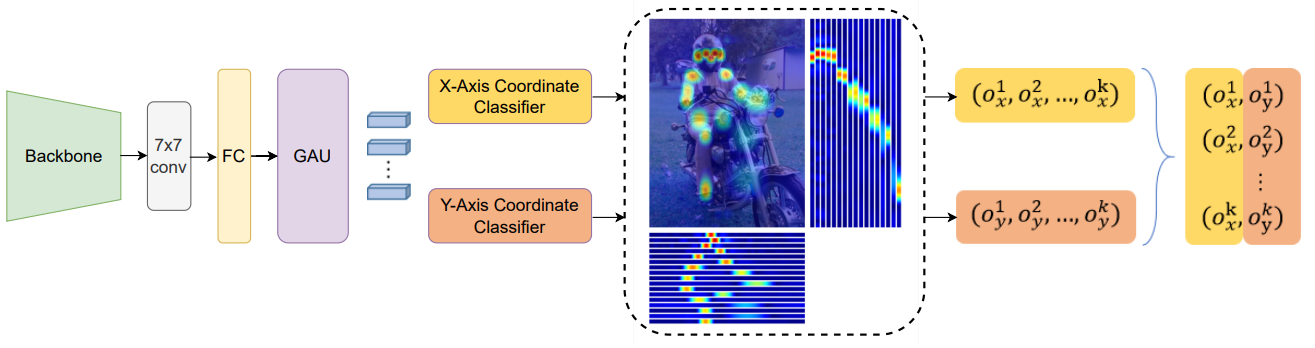
\includegraphics[width=\textwidth]{obrazky-figures/rtmpose_architecture.png}
    \caption{Architecture of the RTMPose models, which comprises of a CSPNeXt backbone, a convolutional layer, a fully-connected layer, and a Gated Attention Unit (GAU) designed to enhance K keypoint representations. Subsequently, the process of 2D pose estimation is treated as two separate classification tasks for the x-axis and y-axis coordinates. This involves predicting the horizontal and vertical positions of keypoints. Taken from \cite{rtmpose}.}
    \label{fig:rtmpose_architecture}
\end{figure}

For prediction of the keypoints, the RTMPose models utilize the SimCC \cite{simcc} algorithm. SimCC reformulates human pose estimation as two classification tasks for horizontal and vertical coordinates. To reduce quantization error, SimCC can use a larger number of bins for the classification tasks. This can lead to better accuracy, while still being faster than post-processing methods commonly used with tradional heatmap based pose estimation models.

To better use spatial information, the RTMPose models use a Gated Attention Unit (GAU) \cite{gau} module. The GAU has faster speed, lower memory cost and better accuracy than the commonly used self-attention module, proposed in the Transformer architecture \cite{attentionIsAllYouNeed}.

\subsection{Model Versions}
This work evaluates the following RTMPose models:

\begin{description}
    \item[RTMPose Body8 models:] These models are trained and evaluated on the Body8 dataset consisting of 8 pose estimation datasets (AI Challenger \cite{ai_challenger}, MS-COCO \cite{coco}, CrowdPose \cite{crowdpose}, MPII \cite{mpii}, sub-JHMDB \cite{JHMDB}, Halpe \cite{halpe}, PoseTrack18 \cite{posetrack} and OCHuman \cite{ochuman}). They predict 17 keypoints, as defined in the COCO dataset.
    \item[RTMPose Halpe26 models:] These models are also trained and evaluated on the Body8 dataset. However, they predict 26 keypoints, as defined in the Halpe26 dataset.
    \item[RTMPose WholeBody models:] These models are trained and evaluated on the COCO-WholeBody \cite{coco-wholebody} and UBody \cite{ubody} datasets. They predict 133 keypoints, as defined in the COCO-WholeBody dataset.
\end{description}




\section{HRNet}
\label{hrnet}

The HRNet (High-Resolution Network) \cite{hrnet} pose estimation architecture is characterized by its emphasis on maintaining high-resolution representations throughout the network. Unlike conventional methods that downsample the input image early in the network, HRNet adopts a multi-resolution approach, preserving detailed information essential for accurate pose estimation.

A notable feature of the HRNet pose estimation architecture is its ability to capture both local and global context effectively. The network consists of parallel branches, each processing different resolutions of the input image, and these branches are interconnected, facilitating the exchange of information between different scales. This design allows HRNet to address challenges associated with scale variations in human poses, ensuring robust performance in capturing both fine details and overall pose structure. Figure \ref{fig:hrnet_architecture} shows the architecture of the HRNet models.

\begin{figure}[htbp]
    \centering
    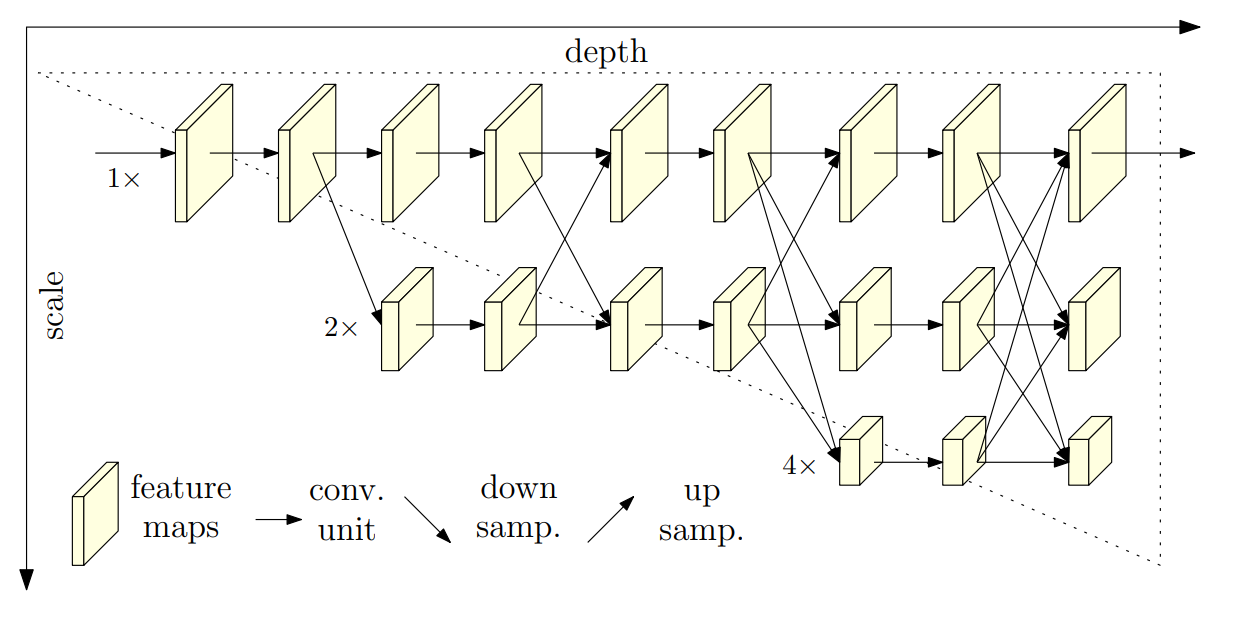
\includegraphics[width=\textwidth]{obrazky-figures/hrnet_architecture.png}
    \caption{Architecture of the HRNet models. The HRNet models consists of three parallel branches, each processing different resolutions of the input image. These branches are interconnected, facilitating the exchange of information between different scales. Taken from \cite{hrnet}.}
    \label{fig:hrnet_architecture}
\end{figure}

This work evaluates the HRNet-W32 model, which uses heatmap to predict the keypoints. The HRNet-W32 model is trained on the COCO dataset and predicts 17 keypoints, as defined in the COCO dataset.


\section{YOLOX-Pose}
\label{yolox-pose}

YOLOX-Pose  is a one-stage human pose estimation model that distinguishes itself from traditional top-down and bottom-up methods. The authors claim that YOLOX-Pose is the first one-stage human pose estimation model that achieves comparable performance to the state-of-the-art two-stage methods.

The one-stage approach has some advantages over bottom-up and top-down approaches. Bottom-up approaches first detect keypoints and then group them into poses. The grouping step is not learned and needs to be hand-crafted. This can lead to inaccurate results, especially in cases where the keypoints from different people are close together.

Top-down approaches first detect people and then predict keypoints for each person. This approach is favored by SOTA models, but the processing time grows linearly with the number of people in the image. This can lead to slow processing times in cases where there are many people in the image. SOTA methods also often use heavy detectors, which further increases the processing time.



The original YOLO-pose \cite{yoloPose} model uses the anchor-based YOLOv5 detector \cite{yolov5}. The YOLOX-Pose model, which is evaluated in this work, uses the YOLOX detector \cite{yolox}. The YOLOX detector is based on the YOLOv5 detector, but uses anchor-free approach, which does not require the anchor boxes to be predefined. This allows the YOLOX detector to be more flexible. The YOLOX detector generally outperforms the YOLOv5 detector on the COCO dataset. Figure \ref{fig:yolopose_architecture} shows the architecture of the YOLOX-Pose model.

\begin{figure}[htbp]
    \centering
    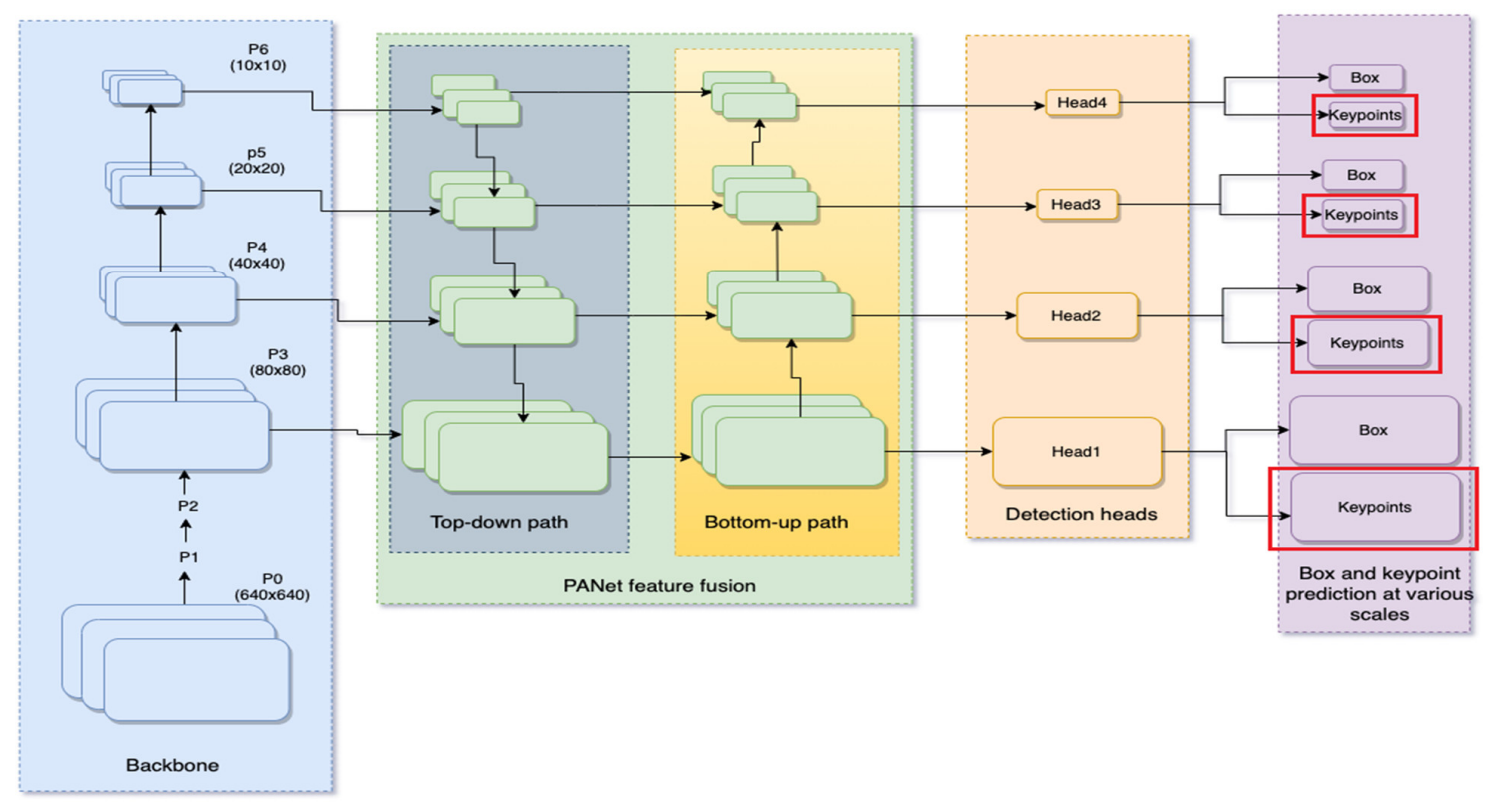
\includegraphics[width=\textwidth]{obrazky-figures/yolopose_architecture.png}
    \caption{Architecture of the original YOLO-Pose model, which was based on the anchor-based YOLOv5 detector. The YOLOX-Pose model, which is evaluated in this work, is based on the anchorless YOLOX detector. Taken from \cite{yoloPose}.}
    \label{fig:yolopose_architecture}
\end{figure}

The YOLOX-Pose model is trained on the COCO dataset and predicts 17 keypoints, as defined in the COCO dataset.

\section{ViPNAS}
\label{vipnas}

The ViPNAS (Video Pose Estimation via Neural Architecture Search) \cite{vipnas} model focuses on video pose estimation, employing two networks: S-ViPNet and T-ViPNet.

The S-ViPNet is used on invidual frames and keyframes in the video to predict the keypoints. The lightweight T-ViPNet network is used on non-keyframes to propagate the pose estimations. It extracts features from the current frame and also fuses heatmaps from the previous frame. The fused features are then used to predict the keypoints.

To find the optimal architectures for the S-ViPNet and T-ViPNet networks, the authors used neural architecture search (NAS). The search space for the S-ViPNet network is called the spatial-level search space. It consists of 5 dimensions (depth, width, kernel size, group and attention). The search space for the T-ViPNet network is called the temporal-level search space. It searches for the optimal fusion operation (addition, multiplication or concatenation) and the best stage of features to fuse.

This work evaluates the modified S-ViPNet model with the MobileNetV3 \cite{mobilenetv3} backbone and SimCC \cite{simcc} algorithm instead of predicting heatmaps. The model is trained on the COCO dataset and predicts 17 keypoints, as defined in the COCO dataset.

\section{Results On The COCO Keypoint Dataset}
To compare the potential of the methods, the results of the models on the COCO dataset are shown in table \ref{tab:evaluation_results_coco}. All of the methods were trained only on the COCO dataset and predict the same keypoints. The results are taken from MMPose documentation \cite{mmpose2020}.

The RTMPose models achieve strong results, with the RTMPose-l-256x192 model achieving the best results. The HRNet-W32 model also performs well but it is a much larger and slower model. However, the other lightweight models such as YOLOX-Pose and ViPNAS-MobileNetV3 perform significantly worse than even the medium and small RTMPose models. Overall the RTMPose models show very promising results compared to the other models.

Table \ref{tab:evaluation_params} compares the performance of the models with their computational costs. The RTMPose models are the most computationally efficient. Especially the m model, which achieves similaar results to the HRNet-W32 model, but is much faster and smaller. The YOLOX-Pose model computational costs are higher, because it is a one-stage model, which predicts the keypoints directly from the image. The ViPNAS-MobileNetV3 model is also very small and fast but it achieves significantly worse results than the RTMPose models.

\begin{table}[htbp]

    \centering
    \begin{tabular}{lcccccc}
        \toprule
        Architecture          & Input Size & AP             & AP-50          & AP-75          & AR             & AR-50          \\
        \midrule
        RTMPose-l             & 256x192    & \textbf{0.758} & \textbf{0.906} & \textbf{0.826} & \textbf{0.806} & 0.942          \\
        HRNet\_w32            & 256x192    & 0.749          & 0.906          & 0.821          & 0.804          & \textbf{0.945} \\
        RTMPose-m             & 256x192    & 0.746          & 0.899          & 0.817          & 0.795          & 0.935          \\
        RTMPose-s             & 256x192    & 0.716          & 0.892          & 0.789          & 0.768          & 0.929          \\
        SimCC\_ViPNAS-MBNetv3 & 256x192    & 0.695          & 0.883          & 0.772          & 0.755          & 0.927          \\
        Yoloxpose\_m          & 640x640    & 0.695          & 0.899          & 0.766          & 0.733          & 0.926          \\
        RTMPose-t             & 256x192    & 0.682          & 0.883          & 0.759          & 0.736          & 0.920          \\


        \bottomrule
    \end{tabular}
    \caption{Results of the models on the COCO dataset. The results are sorted by the Average precision (AP). The AP describes the average precision over Object Keypoint Similarity (OKS) thresholds from 0.5 to 0.95 with a step size of 0.05. The AR describes the average recall over OKS thresholds from 0.5 to 0.95 with a step size of 0.05. The AP-50 and AR-50 are the same as AP and AR, but only for OKS threshold of 0.5. Similarly AR-75 is average recall with OKS threshold of 0.75. The results are taken from MMPose documentation \cite{mmpose2020}.}
    \label{tab:evaluation_results_coco}

\end{table}

% TODO: POPIS

\begin{table}[htbp]

    \centering
    \begin{tabular}{lcccc}
        \toprule
        Architecture          & Input Size & AP             & FLOPS(G) & Params(M) \\
        \midrule
        RTMPose-l             & 256x192    & \textbf{0.758} & 4.2      & 28.1      \\
        HRNet\_w32            & 256x192    & 0.749          & 7.7      & 28.5      \\
        RTMPose-m             & 256x192    & 0.746          & 1.9      & 13.9      \\
        RTMPose-s             & 256x192    & 0.716          & 0.7      & 5.7       \\
        SimCC\_ViPNAS-MBNetv3 & 256x192    & 0.695          & 0.8      & 8.6       \\
        Yoloxpose\_m          & 640x640    & 0.695          & 5.8      & 29.3      \\
        RTMPose-t             & 256x192    & 0.682          & 0.4      & 3.5       \\


        \bottomrule
    \end{tabular}
    \caption{Results of the models on the COCO dataset and their computational cost. The results are sorted by the Average precision (AP). The AP describes the average precision over Object Keypoint Similarity (OKS) thresholds from 0.5 to 0.95 with a step size of 0.05. The FLOPS describe the number of floating point operations needed to process the image. The numbers in the table are in billions. The Params describe the number of parameters in the model. The numbers in the table are in millions. The computational cost numbers are obtained using the MMPose library.}
    \label{tab:evaluation_params}

\end{table}


\chapter{Pose Estimation Dataset for Bikefitting}
\label{ch:dataset}
To evaluate and improve the performance of a pose estimation models in the setting of bikefitting, it is necessary to have a dataset that most closely resembles the real-world use case (videos of cyclists pedaling on an indoor trainer, usually in a side view). Since there is no such dataset, a new small dataset was created.

% TODO: schema
\section{Video Acquisition}

To construct the dataset, at first, the author shot 23 videos of himself pedaling on an indoor trainer or leaning on a wall and pedaling a bike. The videos feature both a road bike and a mountain bike. To ensure variety, they were shot on multiple days in different lighting conditions and enviroments, with various camera angles, clothes and riding positions. The videos were shot in FullHD resolution at 30 or 60 FPS using a Redmi Note 10 Pro smartphone. Both the standard and ultra-wide camera lens were used. The videos are 8-35 seconds long. Figure \ref{fig:examples} shows examples of some of the videos present in the dataset.

\def\imgwidth{0.325\textwidth}

\begin{figure}[htbp]
    \centering
    \begin{subfigure}[b]{\imgwidth}
        \centering

        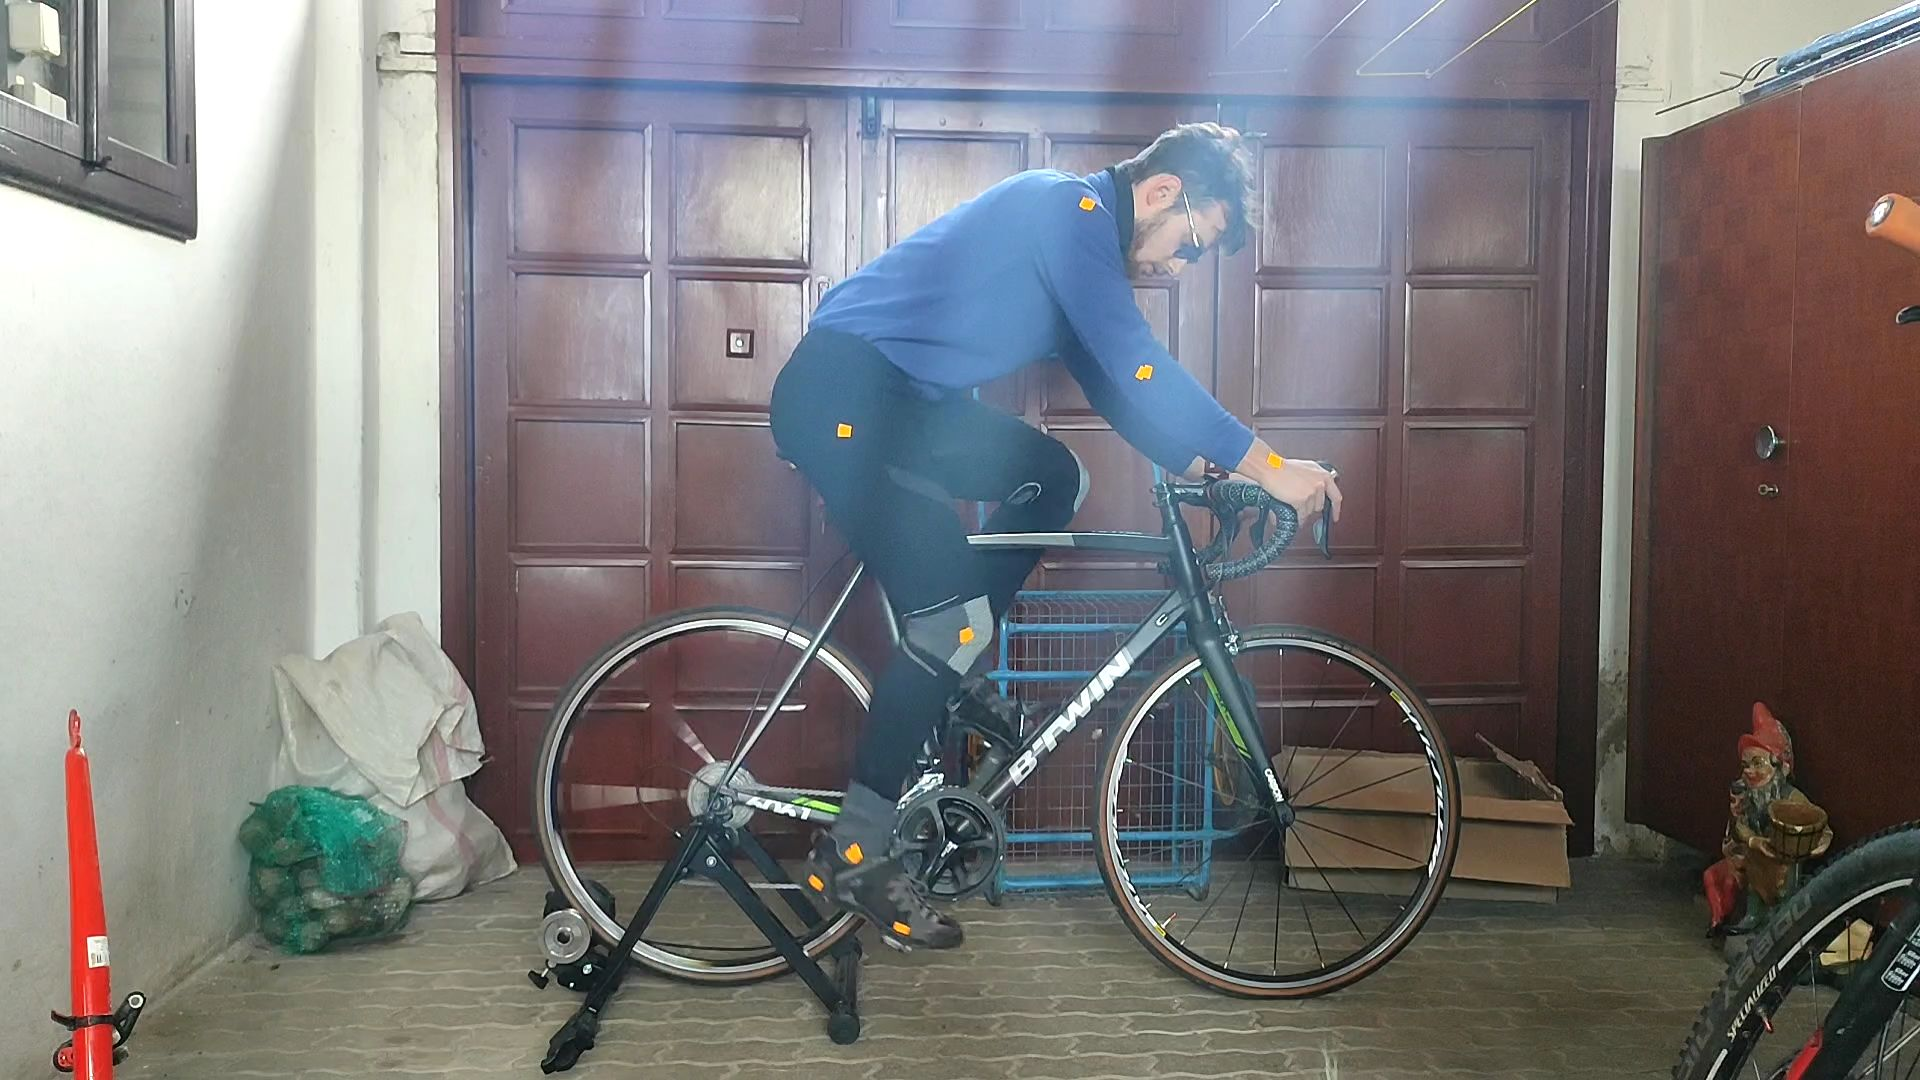
\includegraphics[width=1\linewidth]{obrazky-figures/1.jpg}
        % \caption{MS-COCO keypoints. Taken from \cite{coco}.}

    \end{subfigure}
    \hfill
    \begin{subfigure}[b]{\imgwidth}
        \centering

        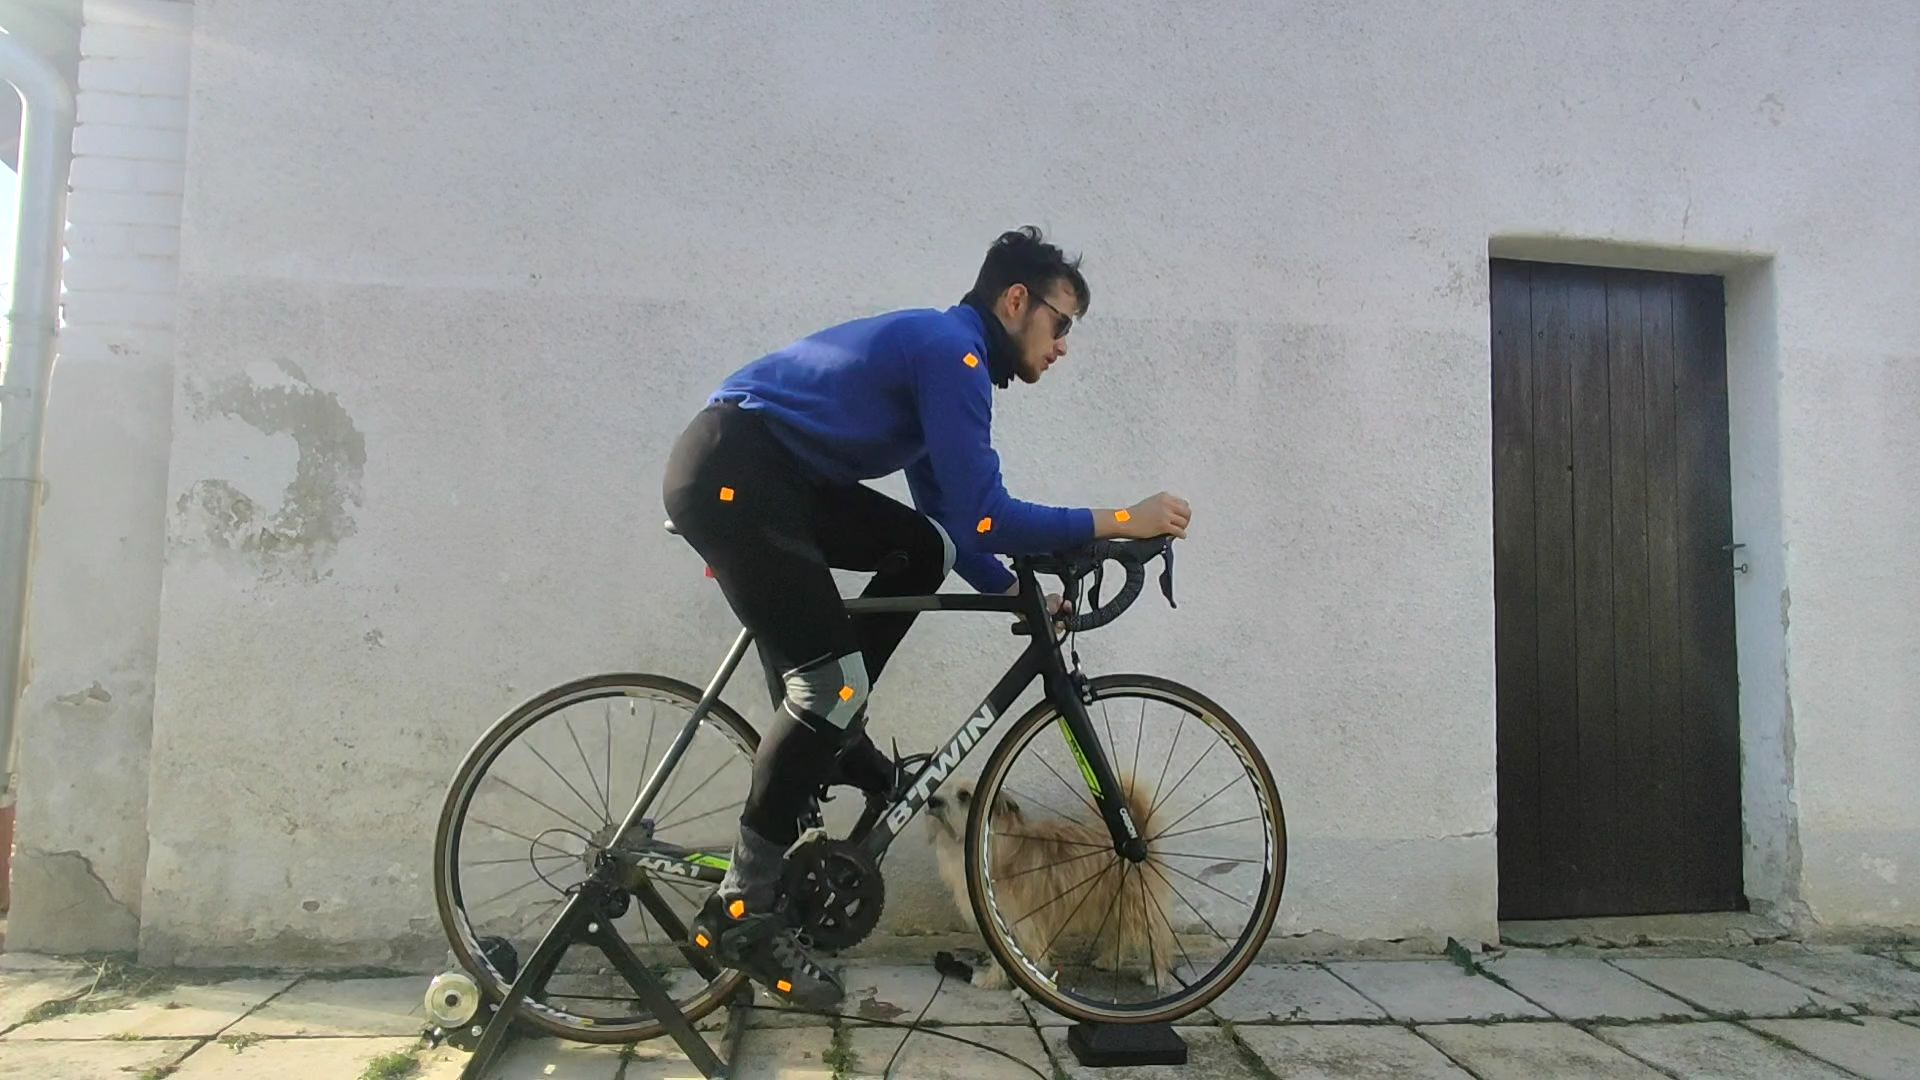
\includegraphics[width=1\linewidth]{obrazky-figures/2.jpg}
        % \caption{MS-COCO keypoints. Taken from \cite{coco}.}

    \end{subfigure}
    \hfill
    \begin{subfigure}[b]{\imgwidth}
        \centering

        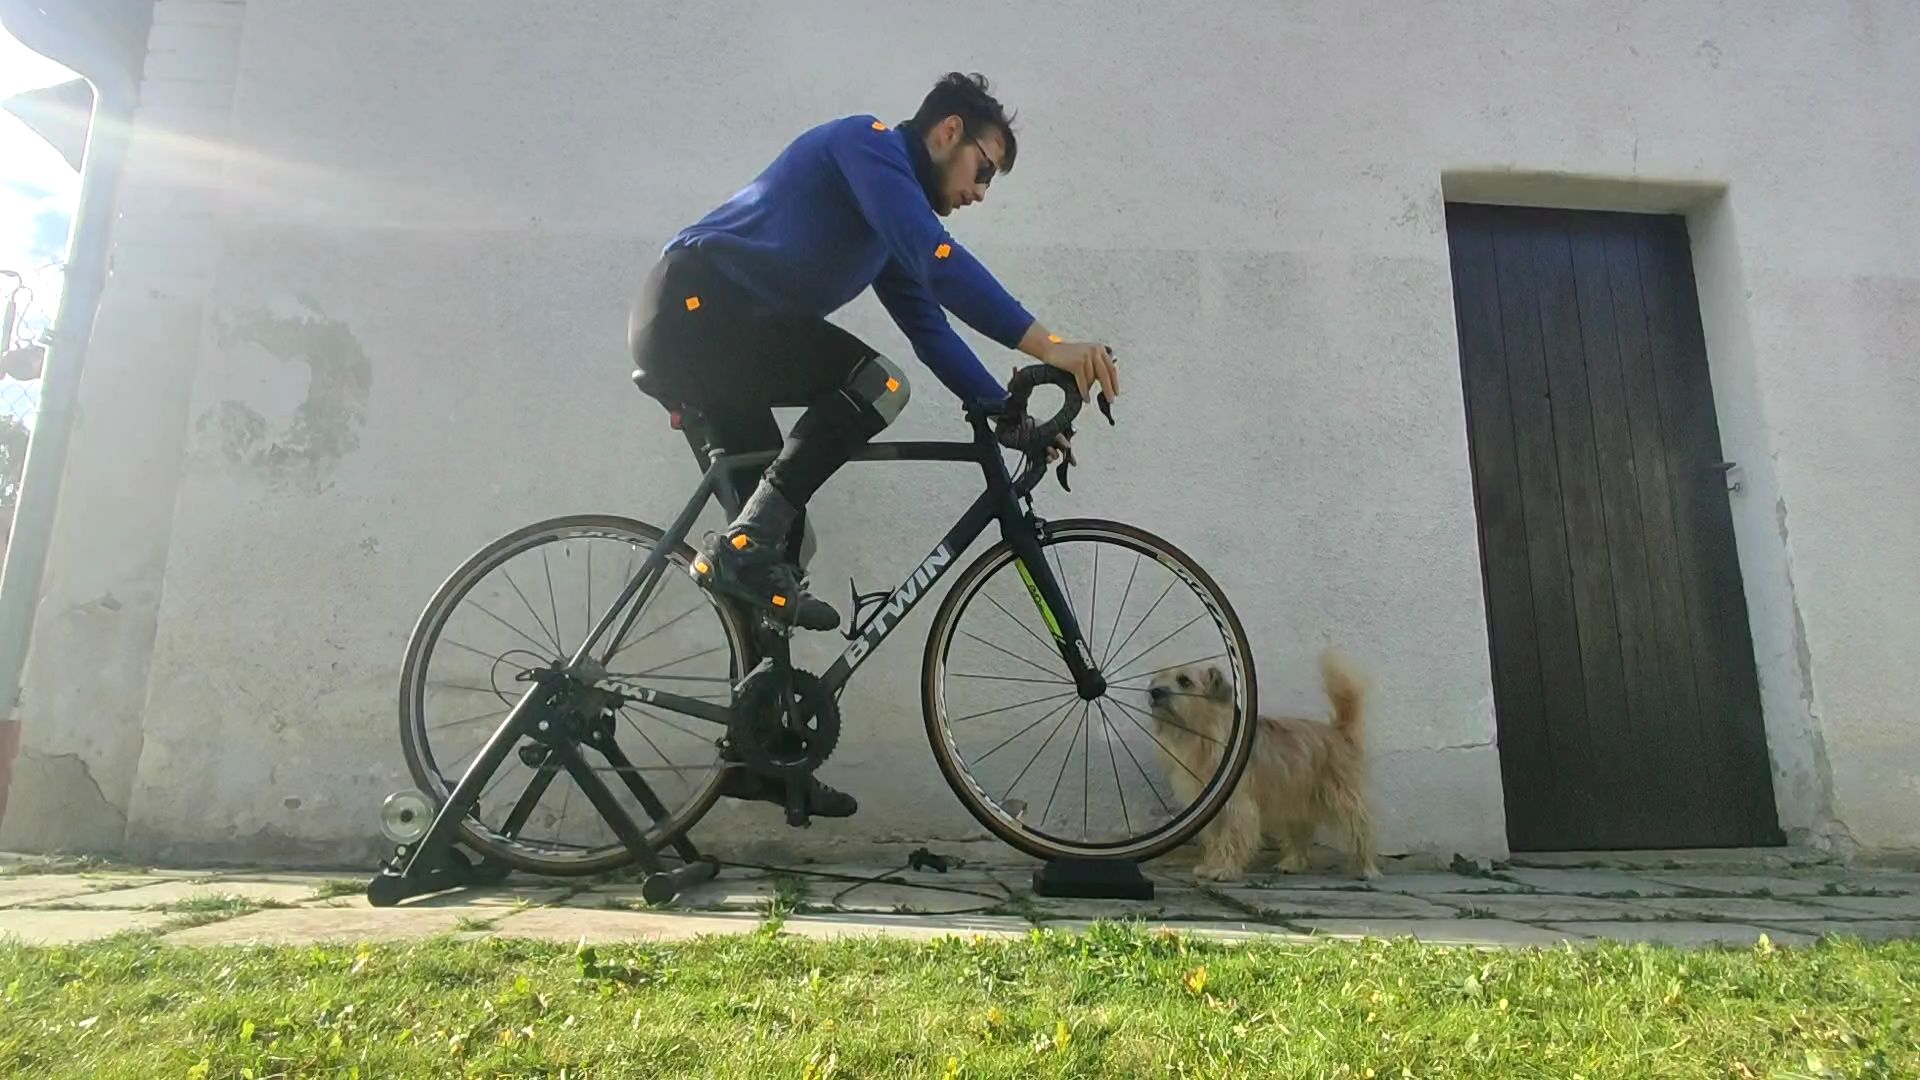
\includegraphics[width=1\linewidth]{obrazky-figures/3.jpg}
        % \caption{MS-COCO keypoints. Taken from \cite{coco}.}
    \end{subfigure}

    \begin{subfigure}[b]{\imgwidth}
        \centering

        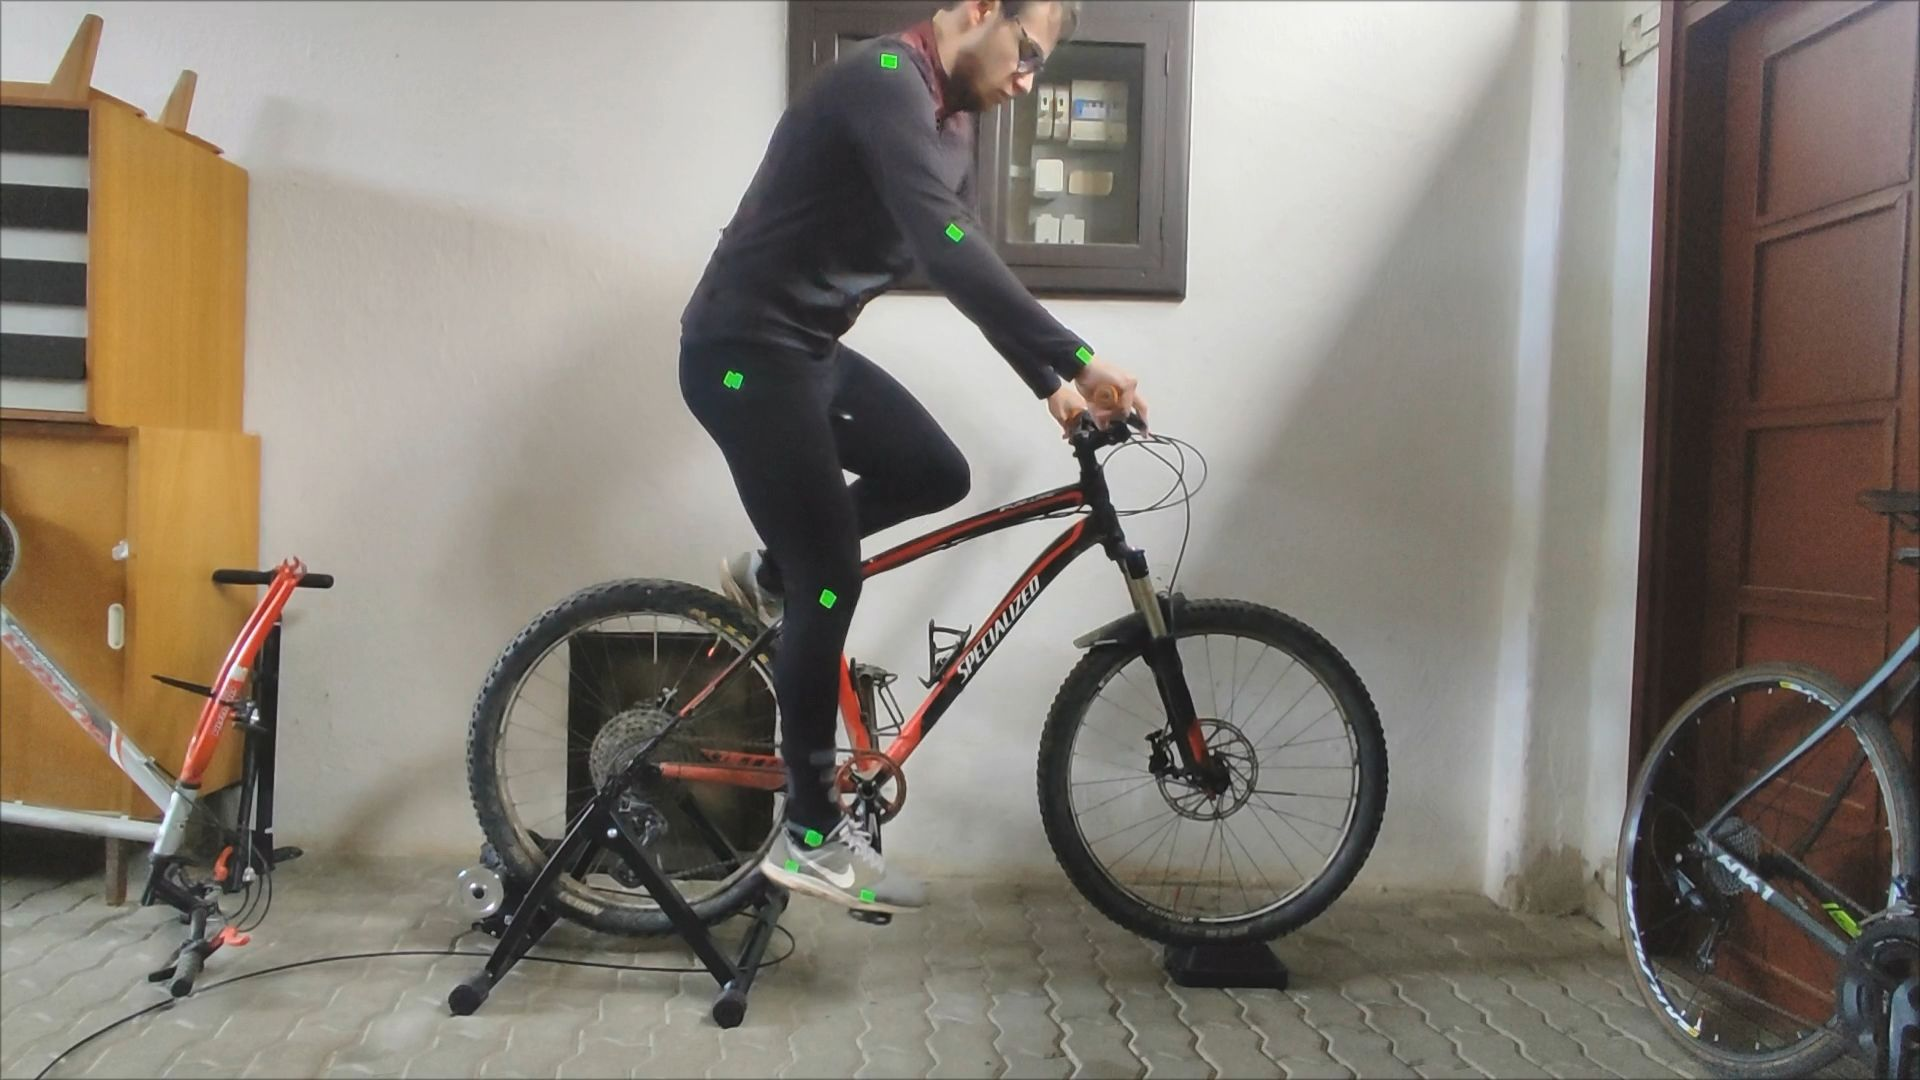
\includegraphics[width=1\linewidth]{obrazky-figures/4.jpg}
        % \caption{MS-COCO keypoints. Taken from \cite{coco}.}

    \end{subfigure}
    \hfill
    \begin{subfigure}[b]{\imgwidth}
        \centering

        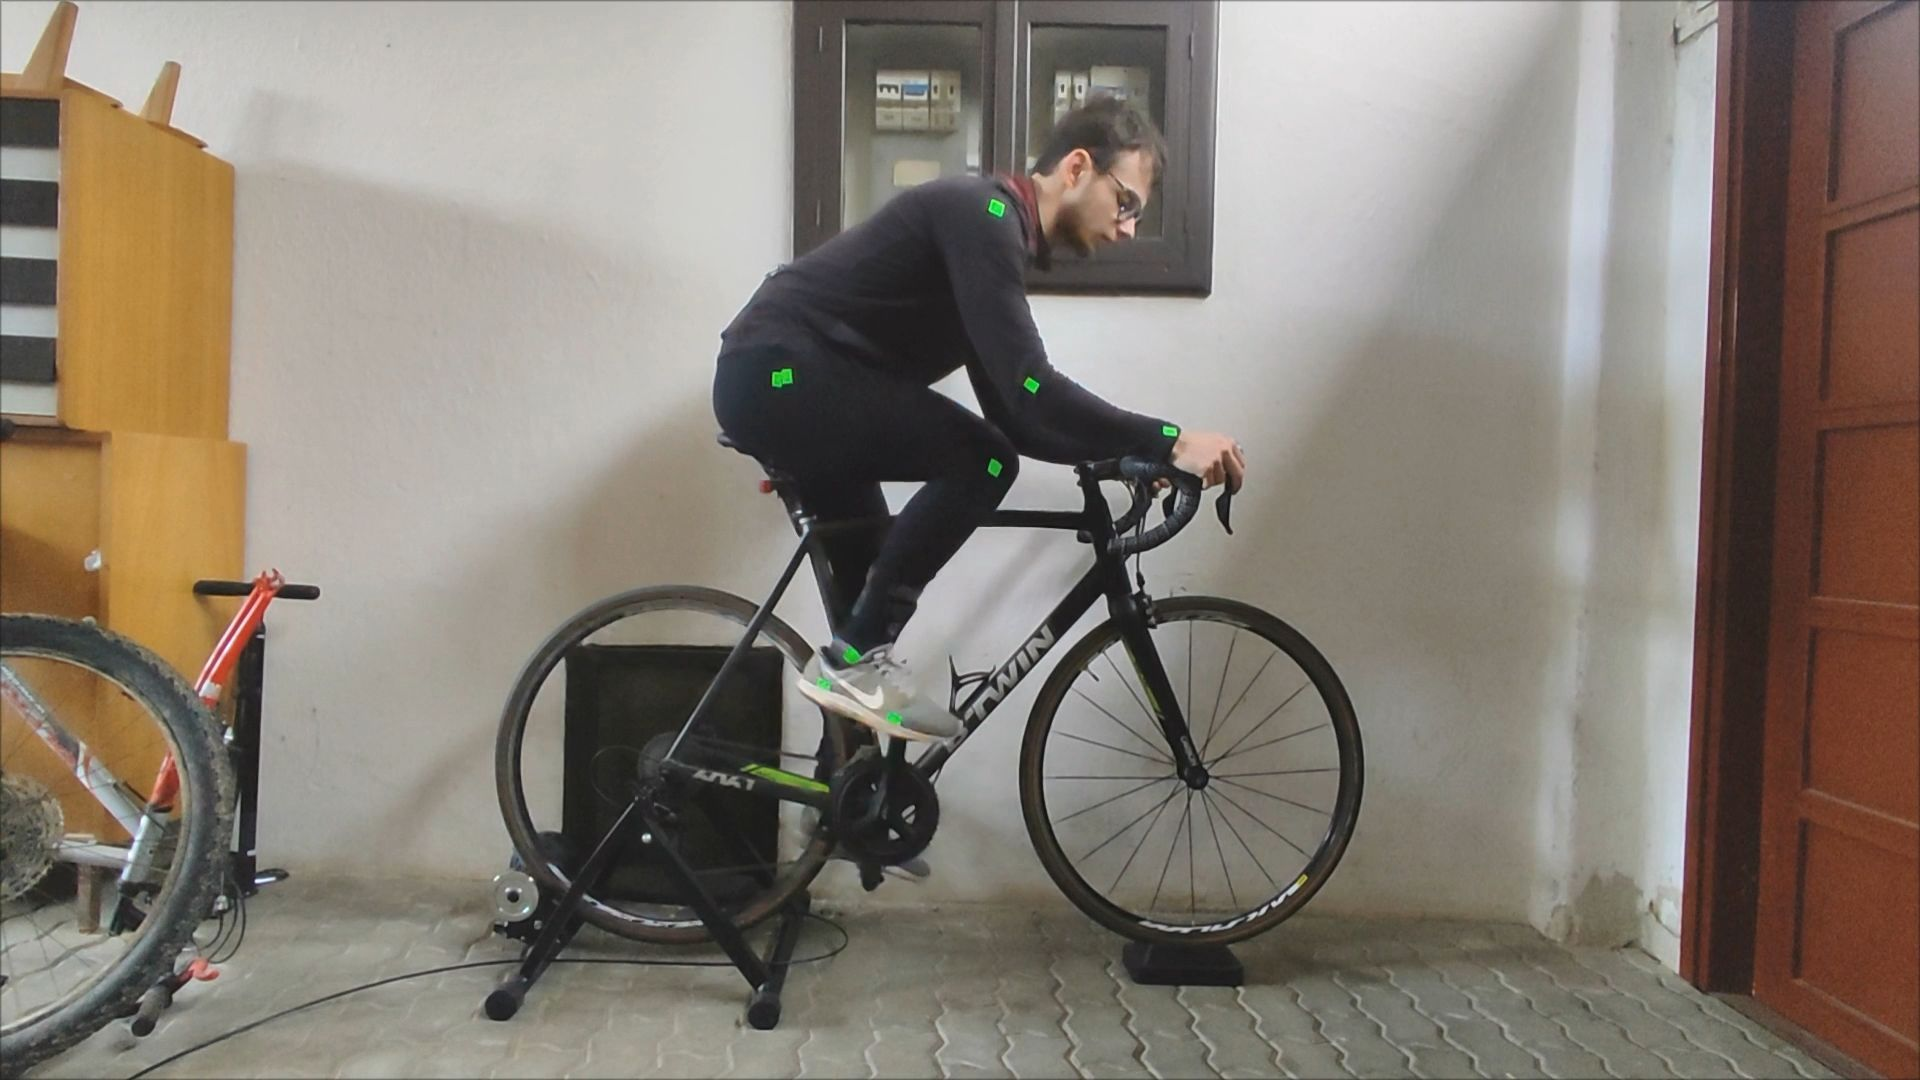
\includegraphics[width=1\linewidth]{obrazky-figures/5.jpg}
        % \caption{MS-COCO keypoints. Taken from \cite{coco}.}

    \end{subfigure}
    \hfill
    \begin{subfigure}[b]{\imgwidth}
        \centering

        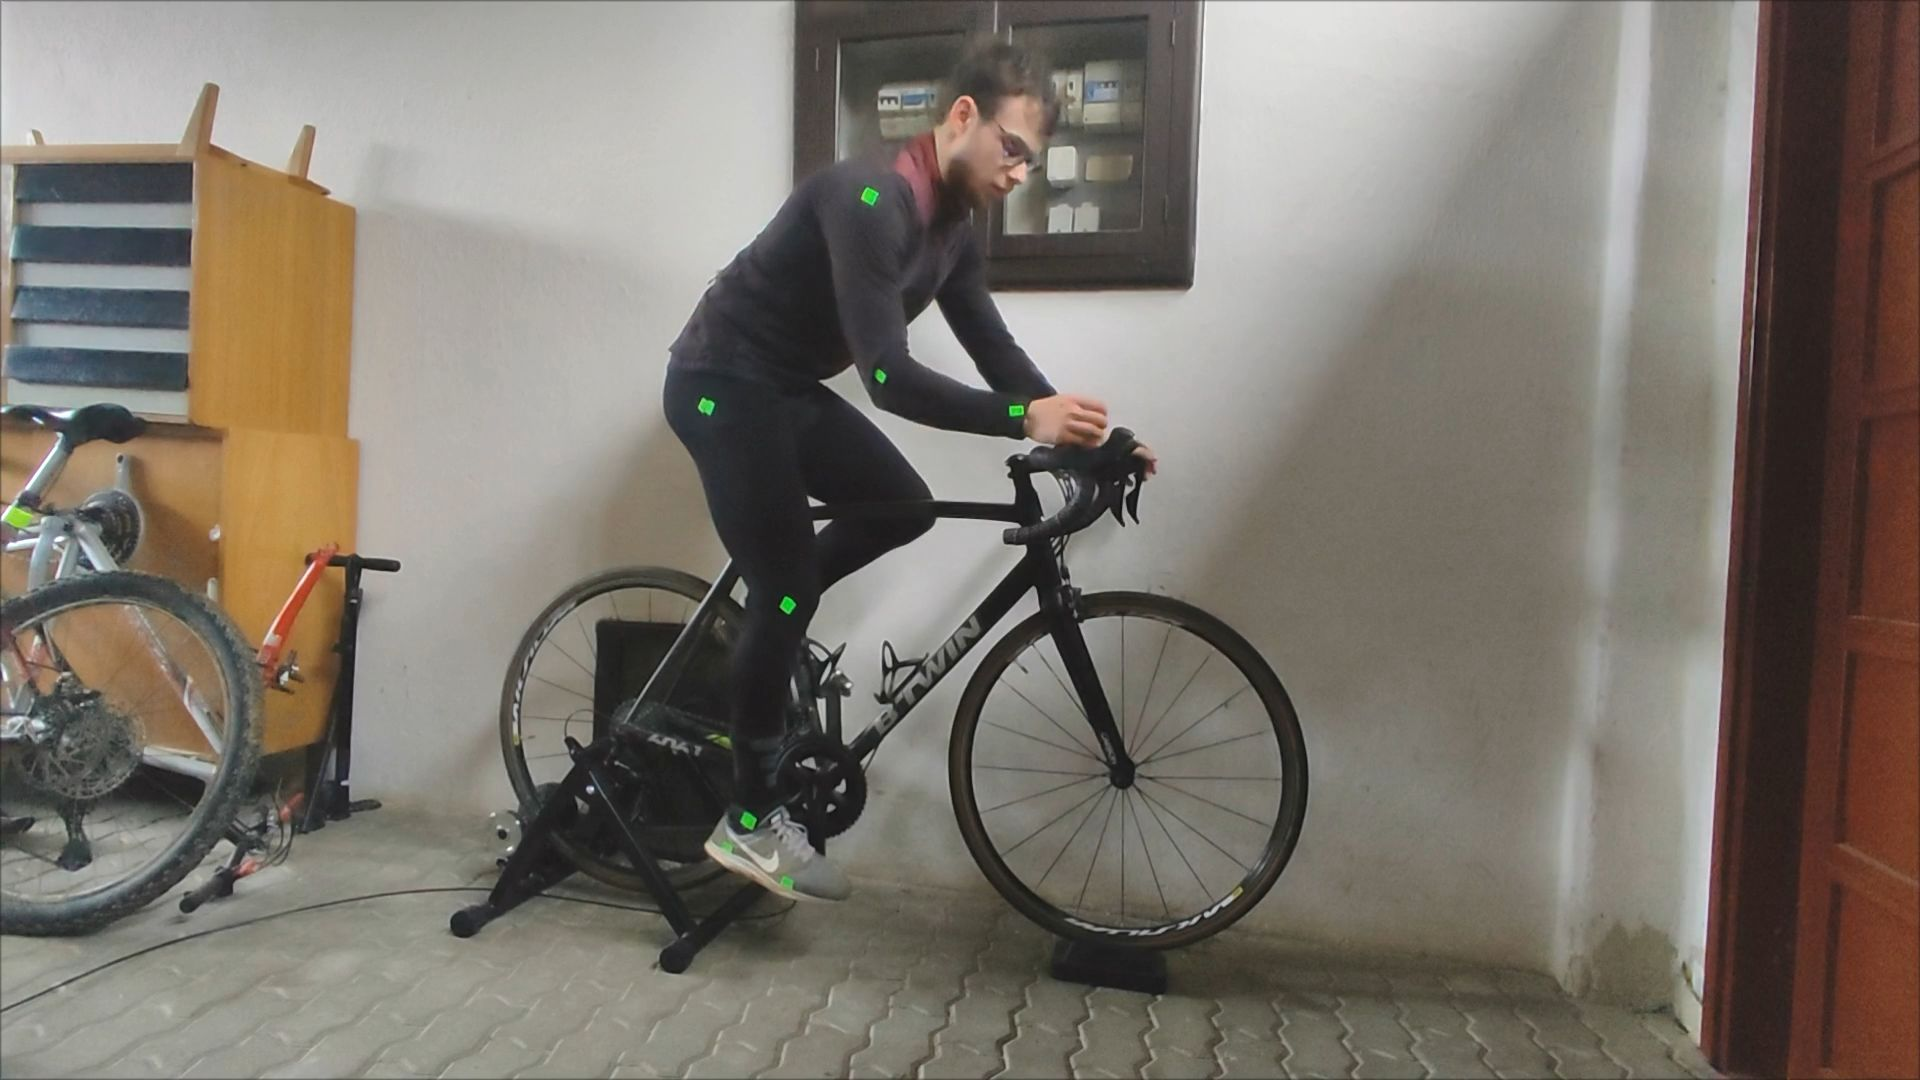
\includegraphics[width=1\linewidth]{obrazky-figures/6.jpg}
        % \caption{MS-COCO keypoints. Taken from \cite{coco}.}
    \end{subfigure}
    \begin{subfigure}[b]{\imgwidth}
        \centering

        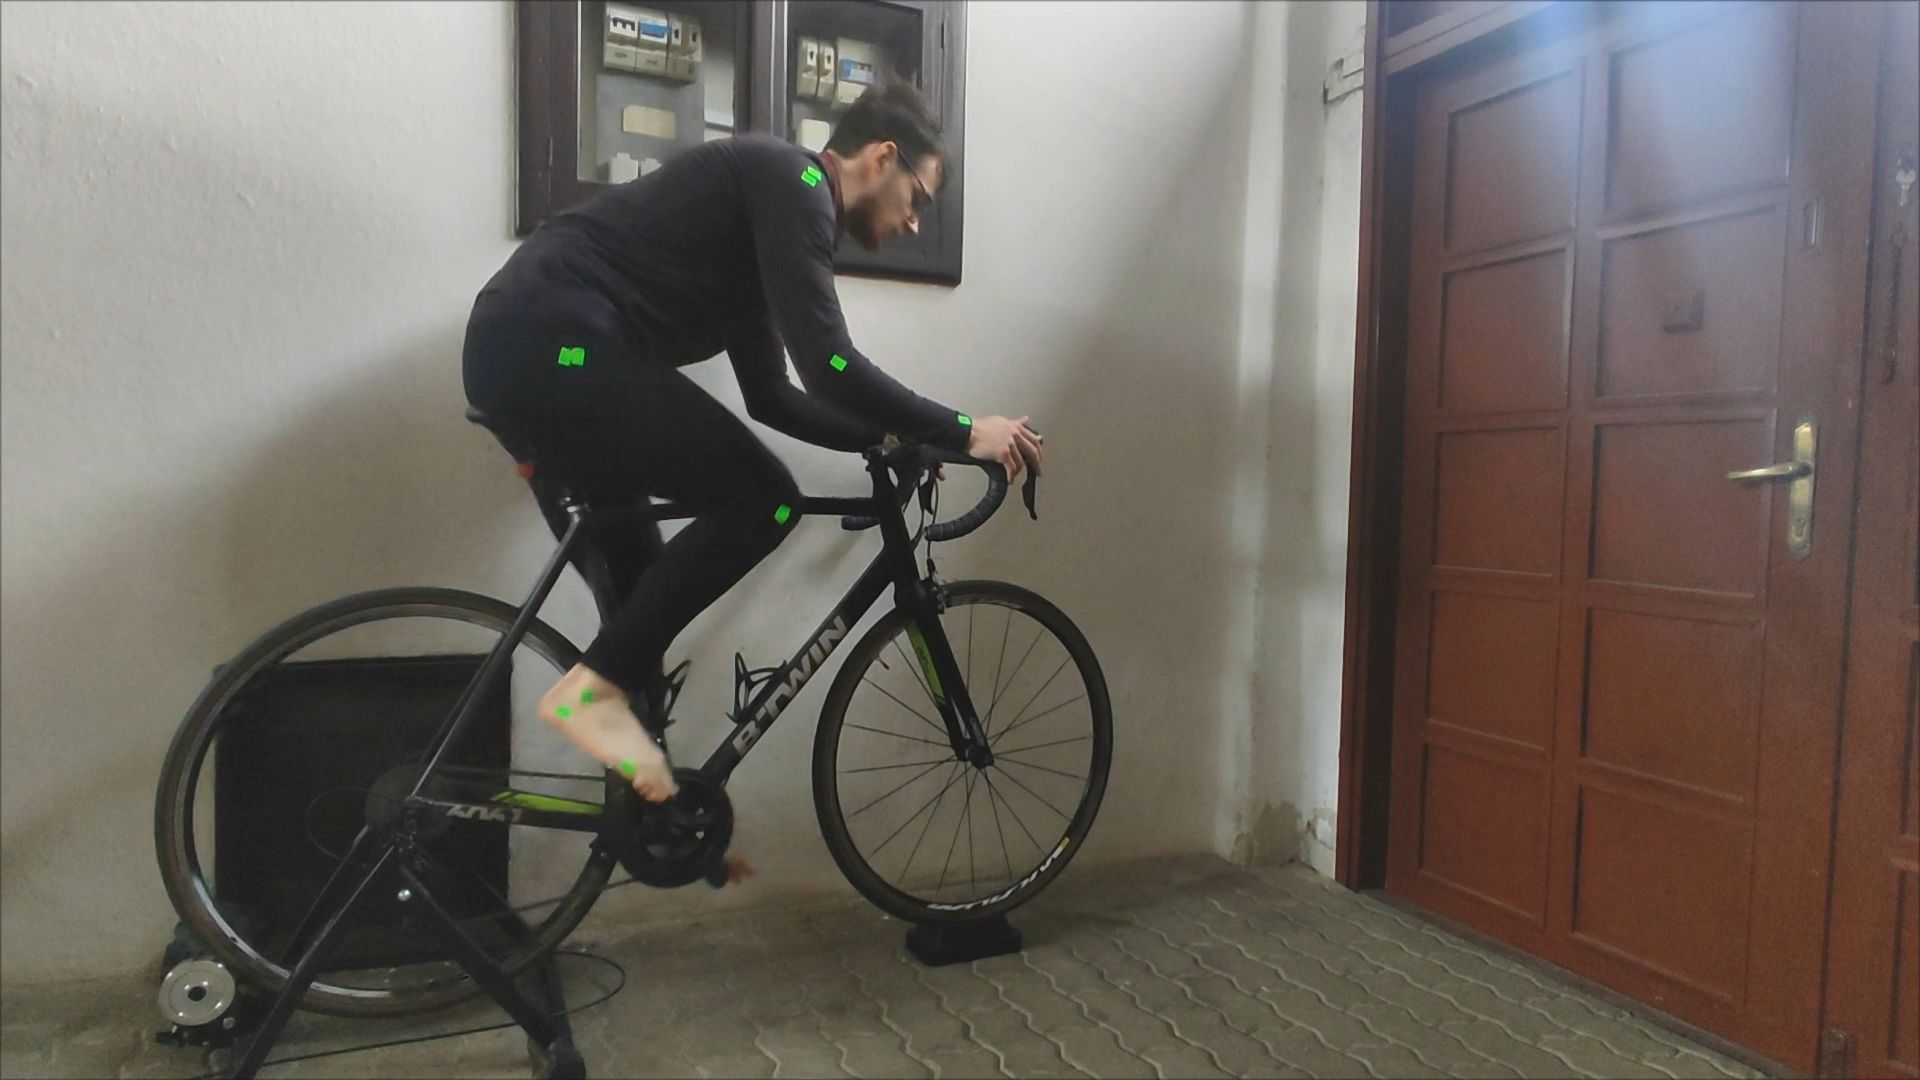
\includegraphics[width=1\linewidth]{obrazky-figures/7.jpg}
        % \caption{MS-COCO keypoints. Taken from \cite{coco}.}

    \end{subfigure}
    \hfill
    \begin{subfigure}[b]{\imgwidth}
        \centering

        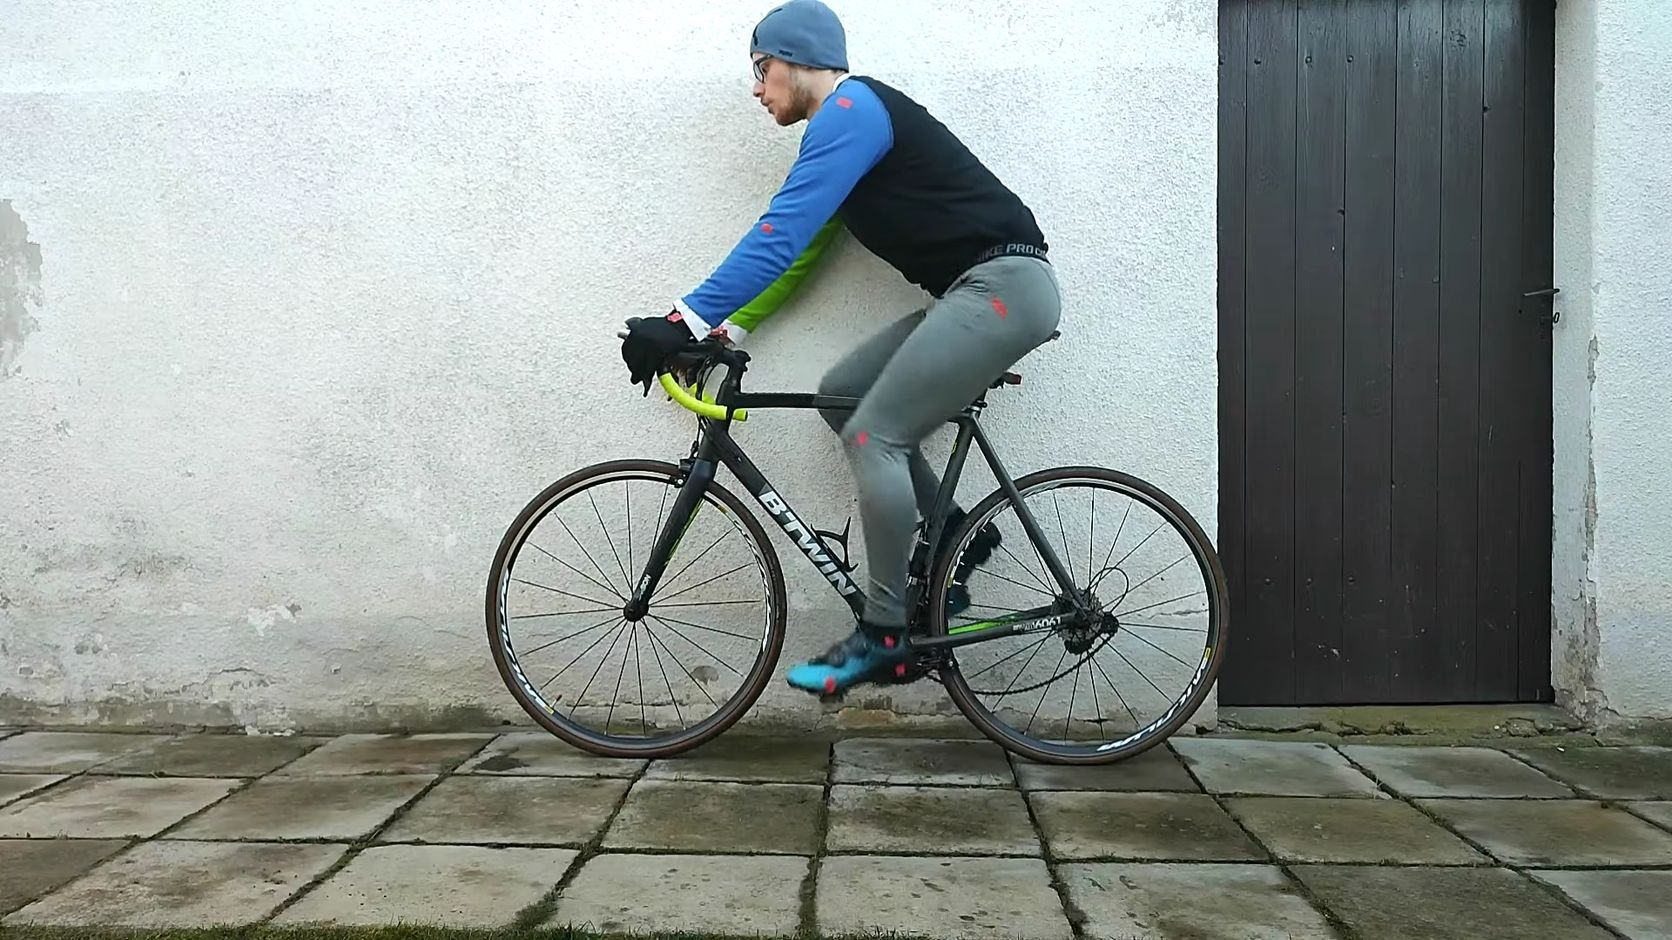
\includegraphics[width=1\linewidth]{obrazky-figures/8.jpg}
        % \caption{MS-COCO keypoints. Taken from \cite{coco}.}

    \end{subfigure}
    \hfill
    \begin{subfigure}[b]{\imgwidth}
        \centering

        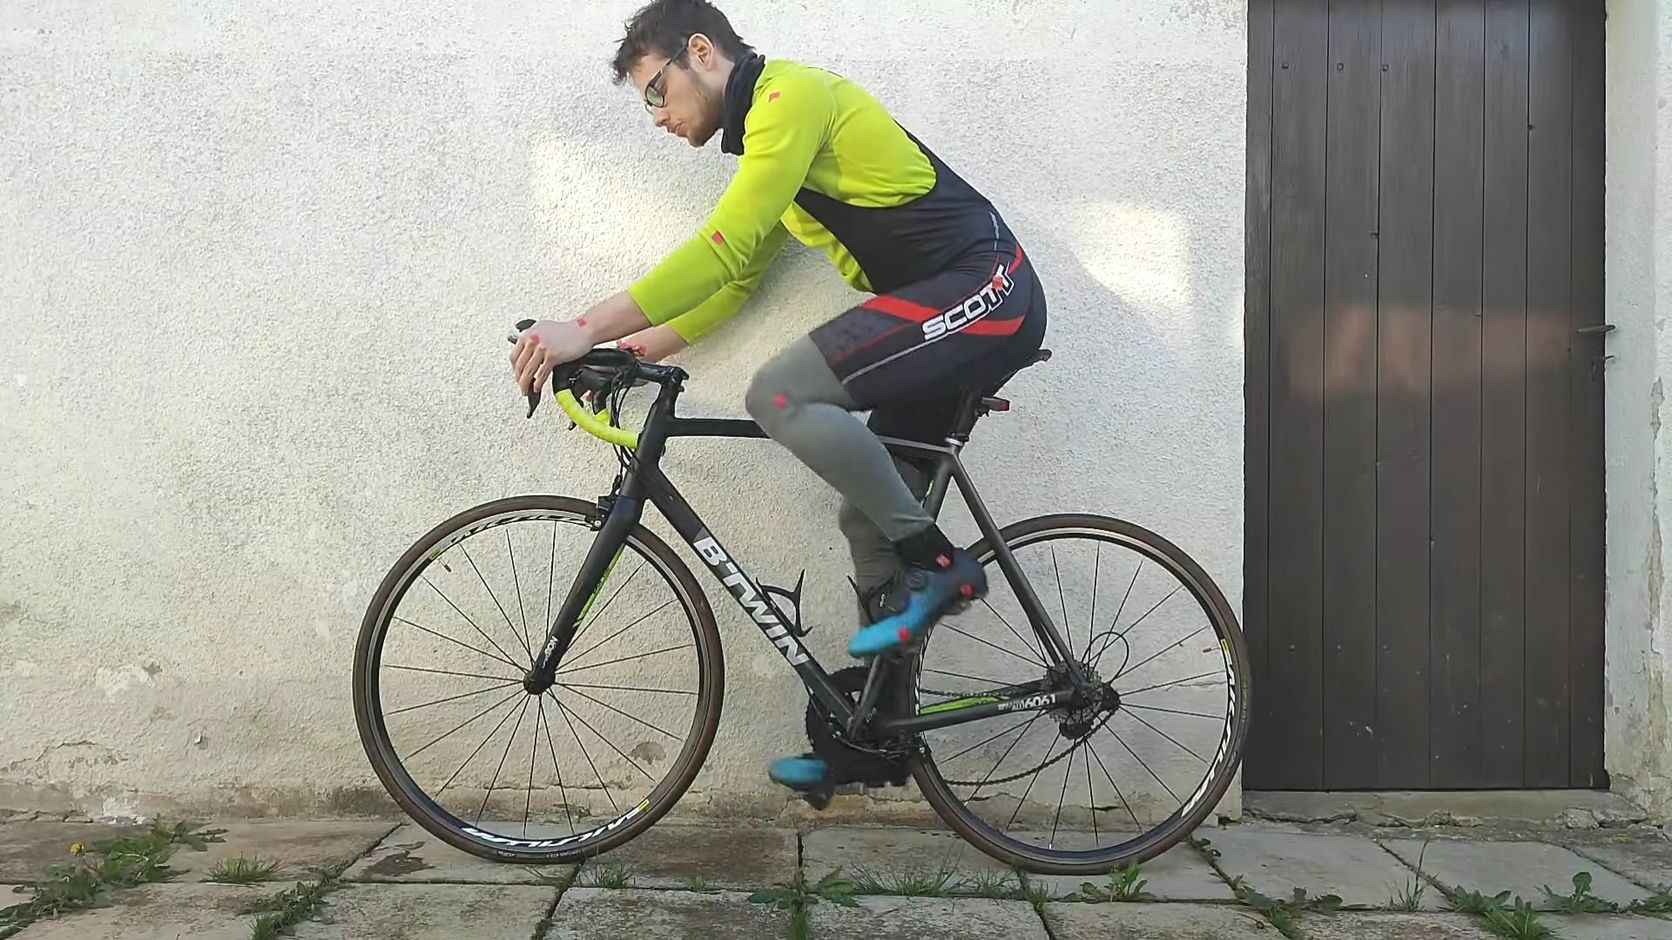
\includegraphics[width=1\linewidth]{obrazky-figures/9.jpg}
        % \caption{MS-COCO keypoints. Taken from \cite{coco}.}
    \end{subfigure}


    \caption{Examples of some the videos present in the dataset. The videos feature both a road bike and a mountain bike. The videos were shot on multiple days in different lighting conditions and enviroments, with various camera angles, clothes and riding positions.}
    \label{fig:examples}
\end{figure}




\section{Obtaining Ground Truth Annotations}
Before shooting the videos, orange colored markers were placed on the camera-facing side of the rider's body. These markers were placed on the following locations: fifth metatarsal of the foot, heel, ankle, knee, hip, shoulder, elbow and wrist. Manually placing markers should be more accurate than annotating the keypoints in the video. The marker placement was guided by the instructions from the Retül bike fitting system \footnote{\url{https://youtu.be/kF0ZjtpO4FE?si=JRLX7lDNZ72oTaiC}}. These markers were the tracked using the methodology described in chapter \ref{marker_based_tracking}. The application tracks the markers in a lower resolution. To get the ground truth annotations, the marker positions were then scaled to the original resolution of the video.

% \begin{figure}[htbp]

%     \centering
%     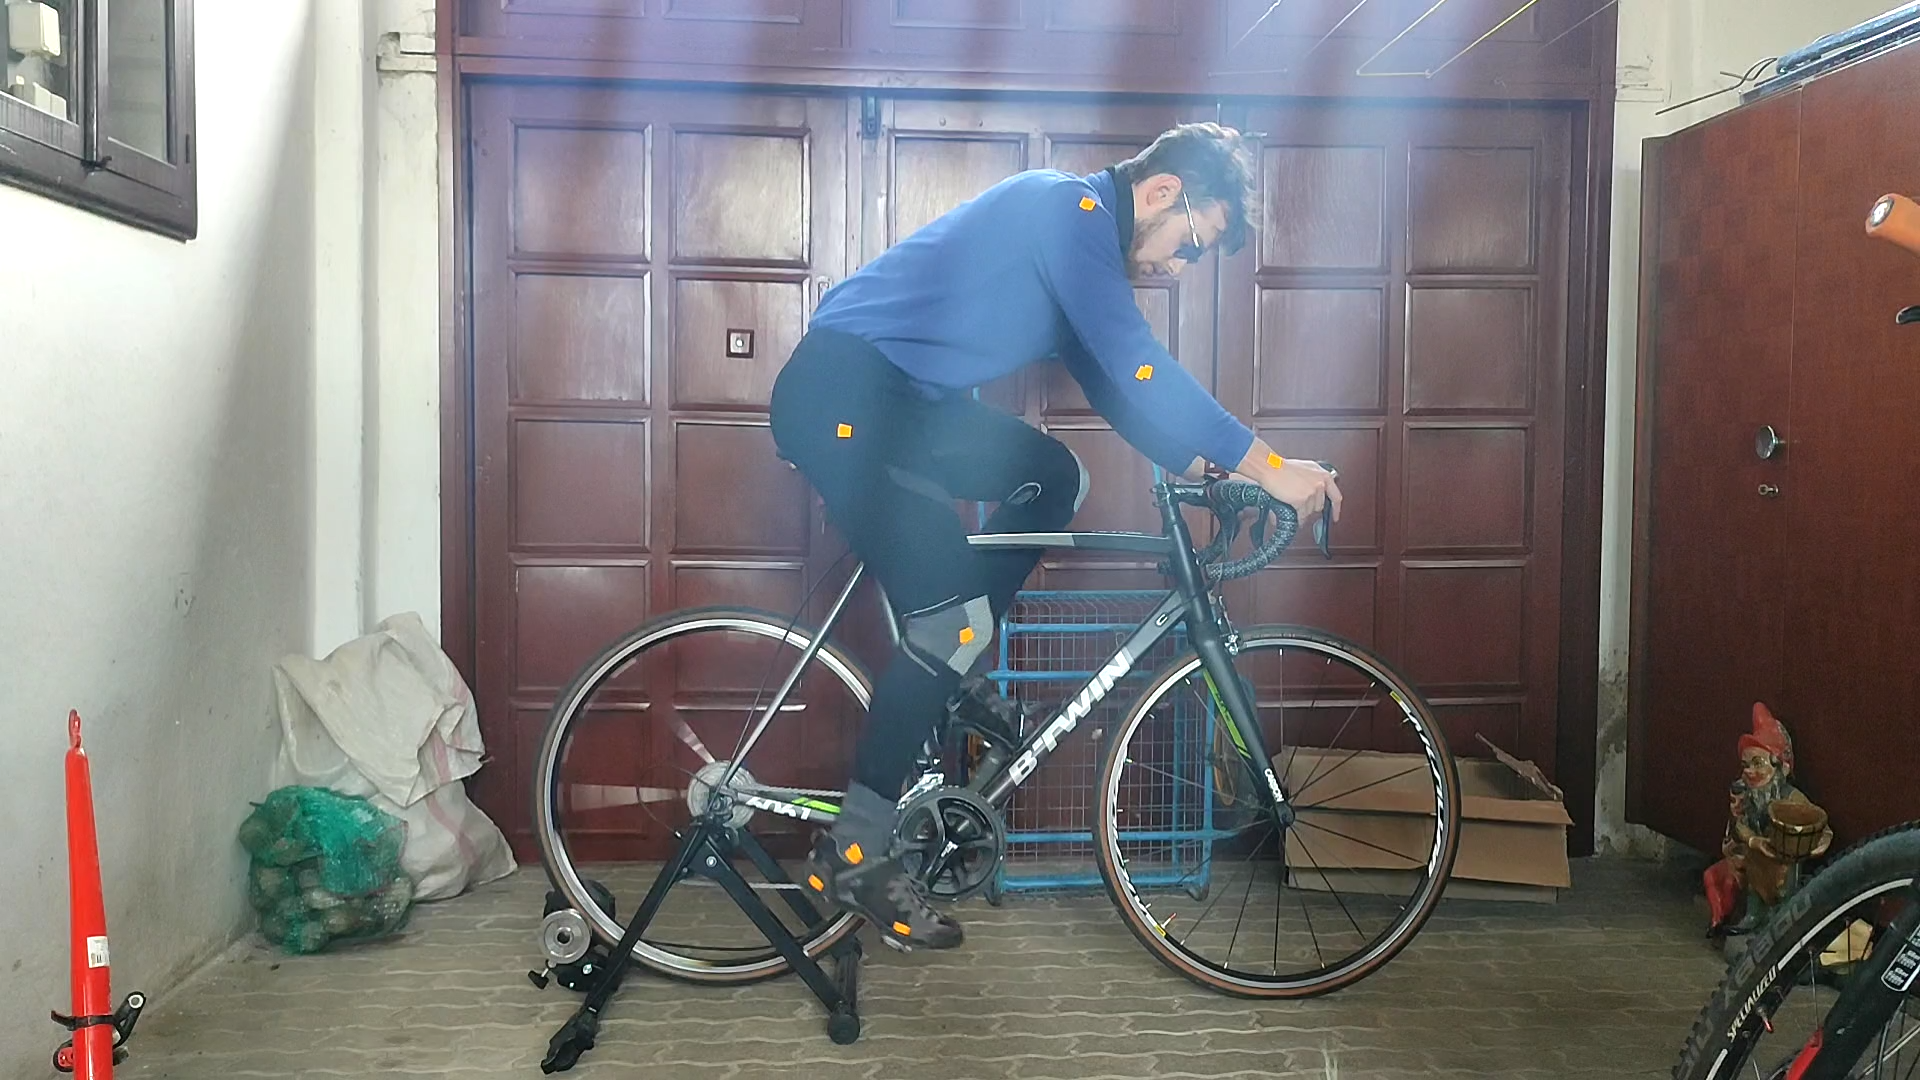
\includegraphics[width=1\linewidth]{obrazky-figures/eval_dataset_in_hoods.png}

%     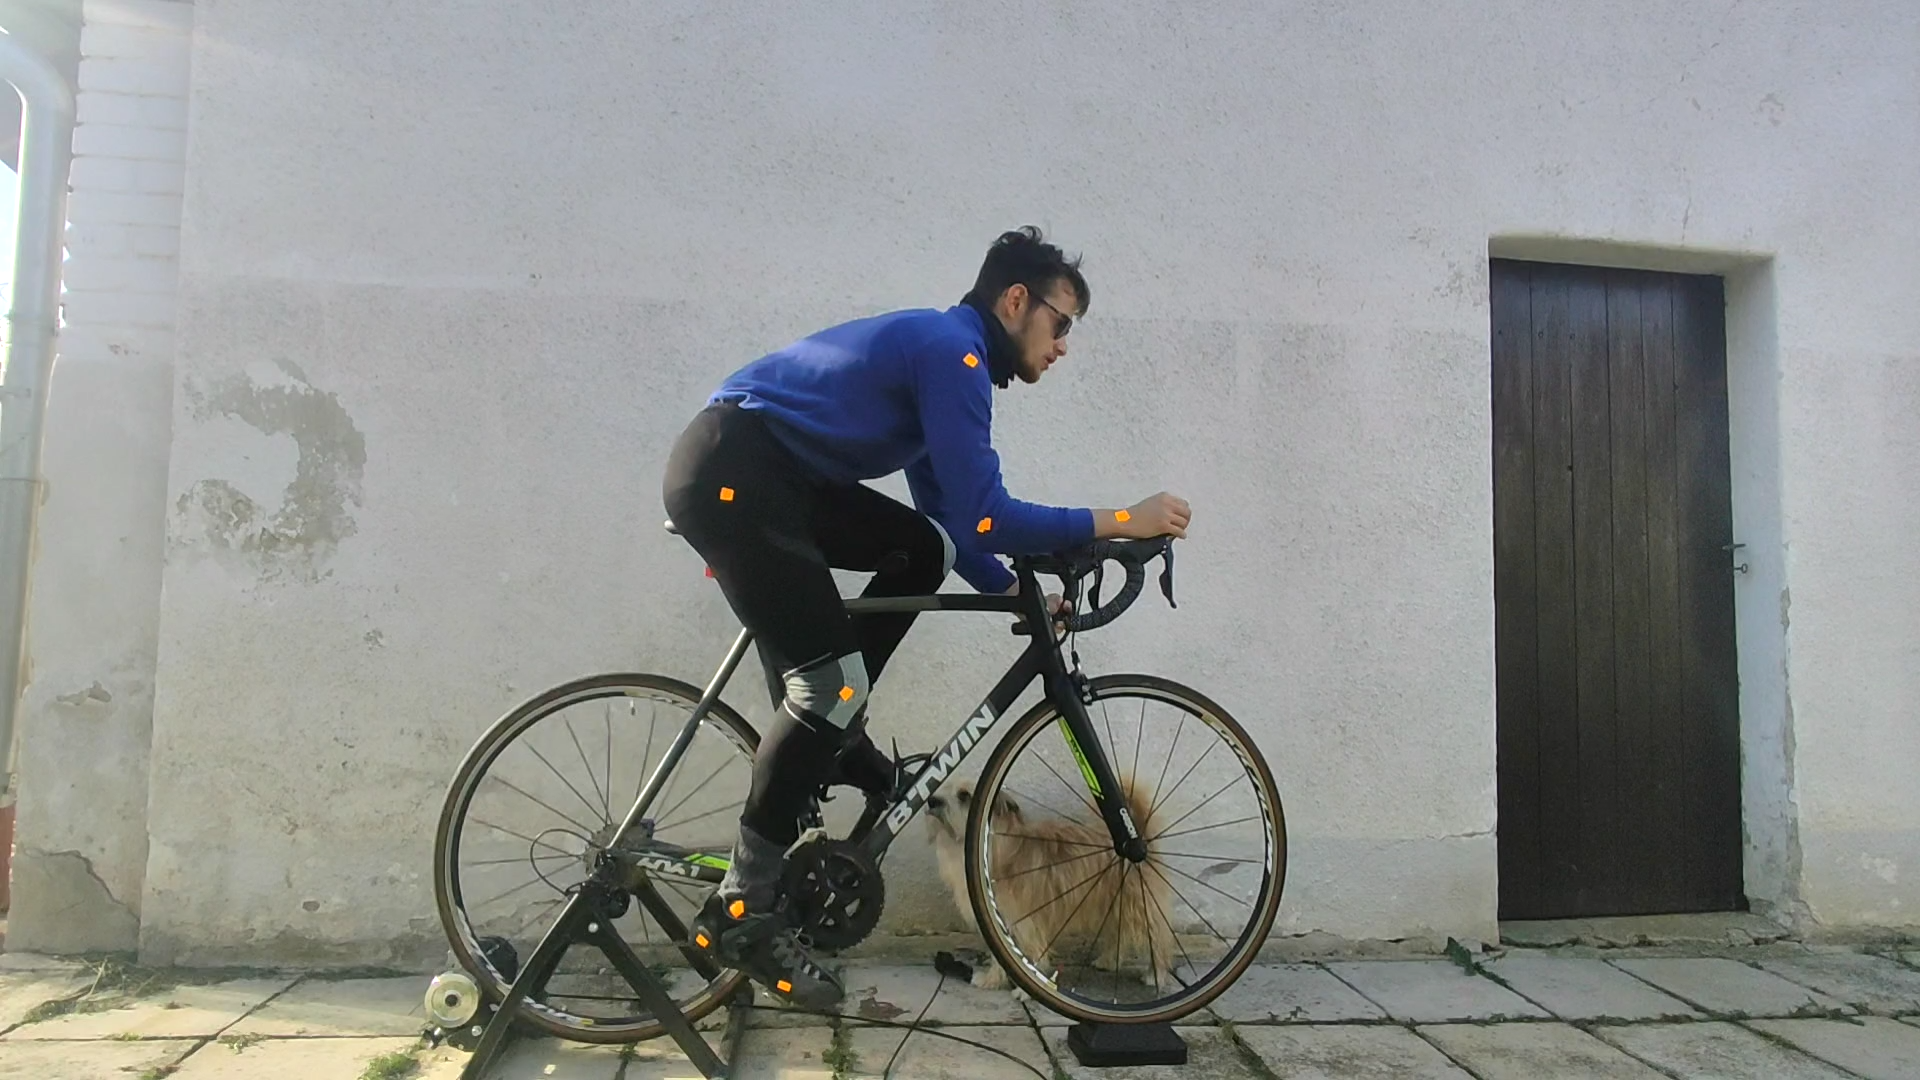
\includegraphics[width=1\linewidth]{obrazky-figures/eval_dataset_out_aero.png}

%     \caption{Examples of the evaluation dataset. The first video shows the rider pedaling indoors on the hoods. The second video shows the rider pedaling outdoors in the aero position on the hoods. The orange stickers are used as ground truth annotations.}


%     \label{fig:evaluation_markers}
% \end{figure}


After obtaining annotations for the 8 markers facing the camera, the annotations for the remaining keypoints need to be obtained. To do this, the RTMPose-l-256x192 model was used to predict the keypoints for the videos. The model was trained on the Body8 dataset and predicts 26 keypoints. These keypoints are not needed for evaluation of the models for bikefitting, but are needed for the fine-tuning of the models. If the models are fine-tuned only on the 8 keypoints, the model will unlearn how to localize the other keypoints. Another reason for predicting the keypoints is to get the bounding box of the person. The bounding box is needed to crop the frames to the bounding box of the person. The bounding box is predicted by the RTMDet-nano model \cite{rtmdet} from the MMDetection framework \cite{mmdetection}. Figure \ref{fig:dataset_annotations} shows an example frame from the dataset with the annotations.

\begin{figure}[htbp]
    \centering
    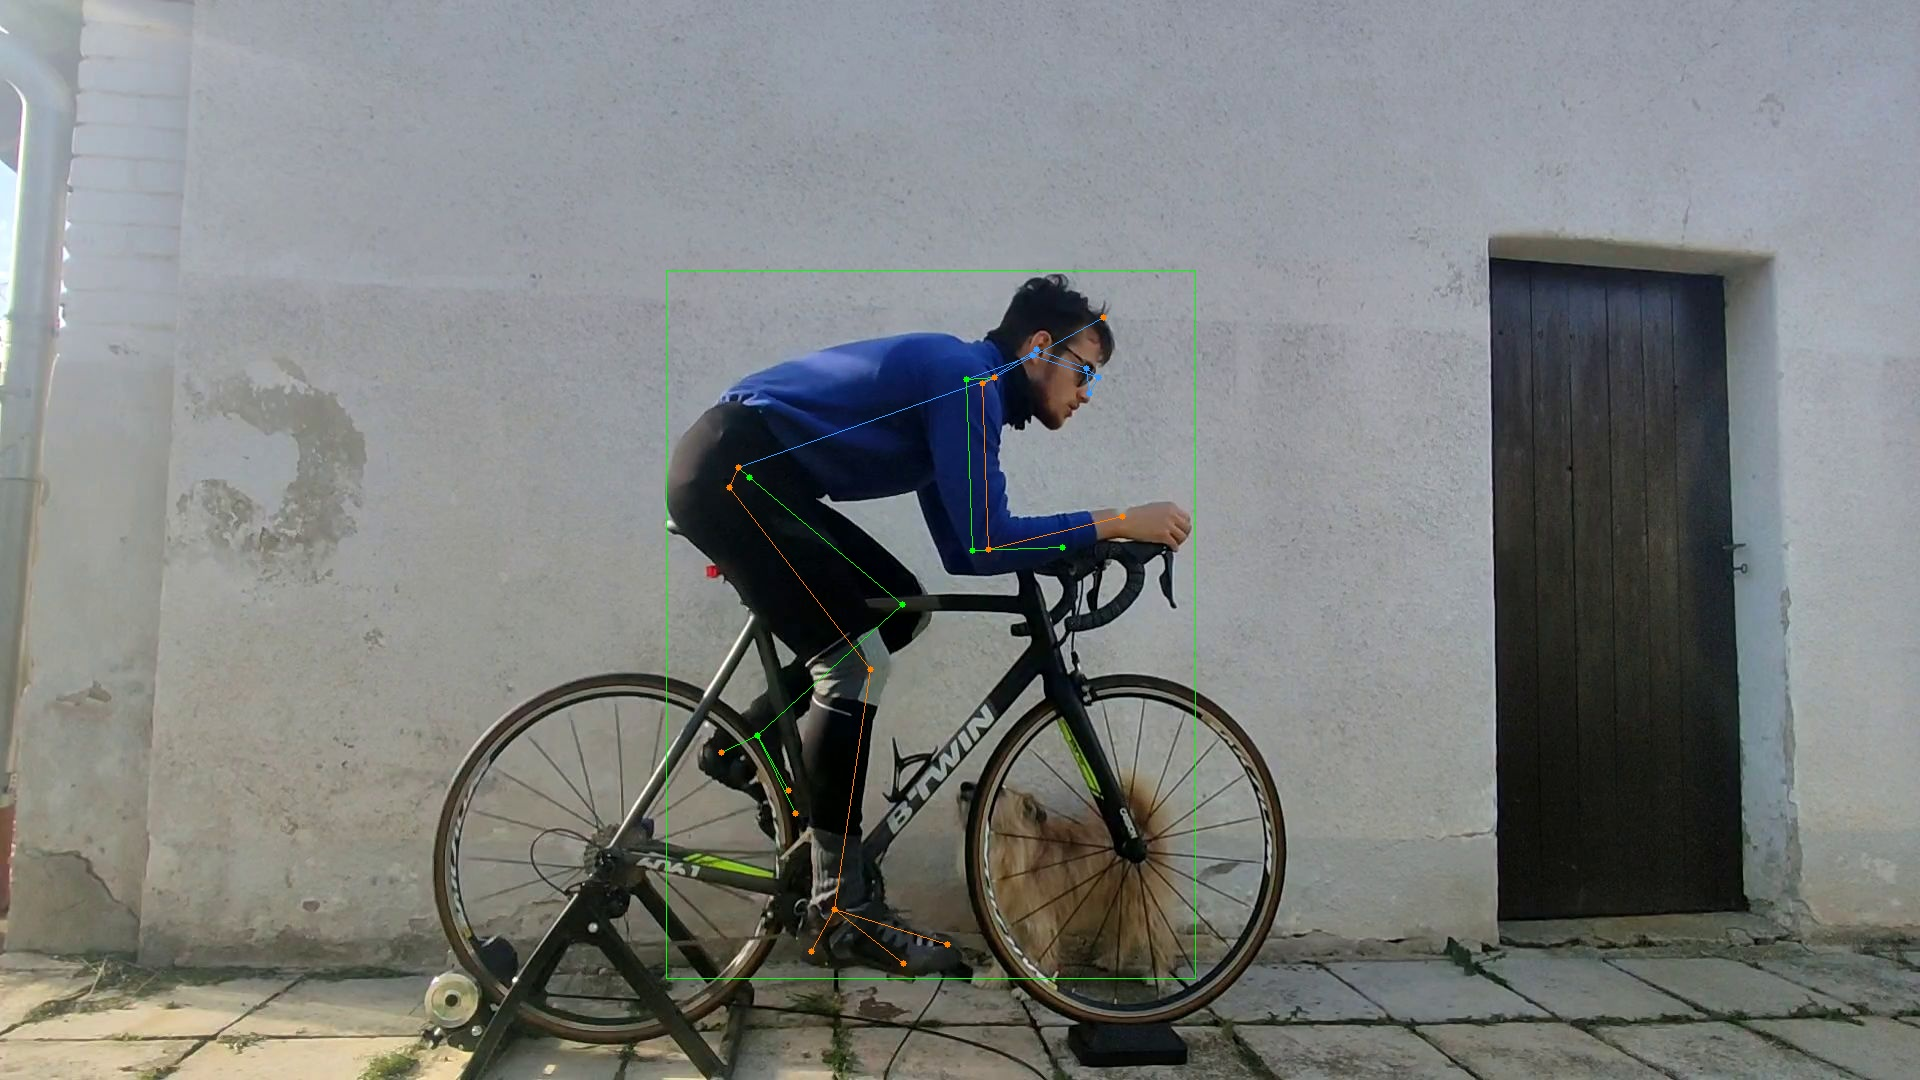
\includegraphics[width=1\linewidth]{obrazky-figures/annotations_1.jpg}

    \caption{Example frame with annotations from the dataset. Ground truth locations of the 8 camera facing keypoints are obtained by tracking colored markers. The remaining keypoints are predicted by the RTMPose-l-256x192 model. The bounding box of the person is obtained by the RTMDet-nano model.}
    \label{fig:dataset_annotations}
\end{figure}



\section{Extracting Individual Frames}
After obtaining the annotations, the individual frames are extracted from the videos. This is done since the pose estimation models are trained on individual frames and not on videos.

To reduce the size of the dataset and remove duplicate frames, not all of the frames are extracted. The frames to extract are selected using the k-means clustering algorithm \cite{kmeans}. Then only the centroids of the clusters are used as the frames for the dataset. The clustering is ran on the locations of the 8 markers. The number of clusters is set to 1/3 of the number of frames.

\section{Removing Colored Markers From the Frames}
To not bias the training and evaluation of the models, the colored markers are removed from the frames. This is done using an inpainting algorithm. The inpainting algorithm takes the frames with the colored markers and a mask of the colored markers and outputs the frames with the colored markers removed.

The mask of the colored markers is created the same way as in the marker-based tracking method, described in chapter \ref{marker_based_tracking}. It works by converting the frames to the CIELAB color space and thresholding the A and B channels using the minimum and maximum A and B channel values of the colored markers.

The inpainting was done using the opencv library \cite{opencv}. The library contains implementations of the Navier-Stokes inpainting algorithm \cite{ns-inpainting}, which is based on fluid dynamics, and the Fast Marching Method \cite{fast-marching-inpainting}, which works by propagating the information from the known parts of the image to the unknown parts. After testing both algorithms, the Navier-Stokes inpainting algorithm was chosen, as it produced better results. Figure \ref{fig:inpainting} shows an example of the inpainting algorithm. It works well in most cases, but struggles with non-uniform backgrounds and can inpain unwanted parts of the image if the mask is not accurate.

\begin{figure}
    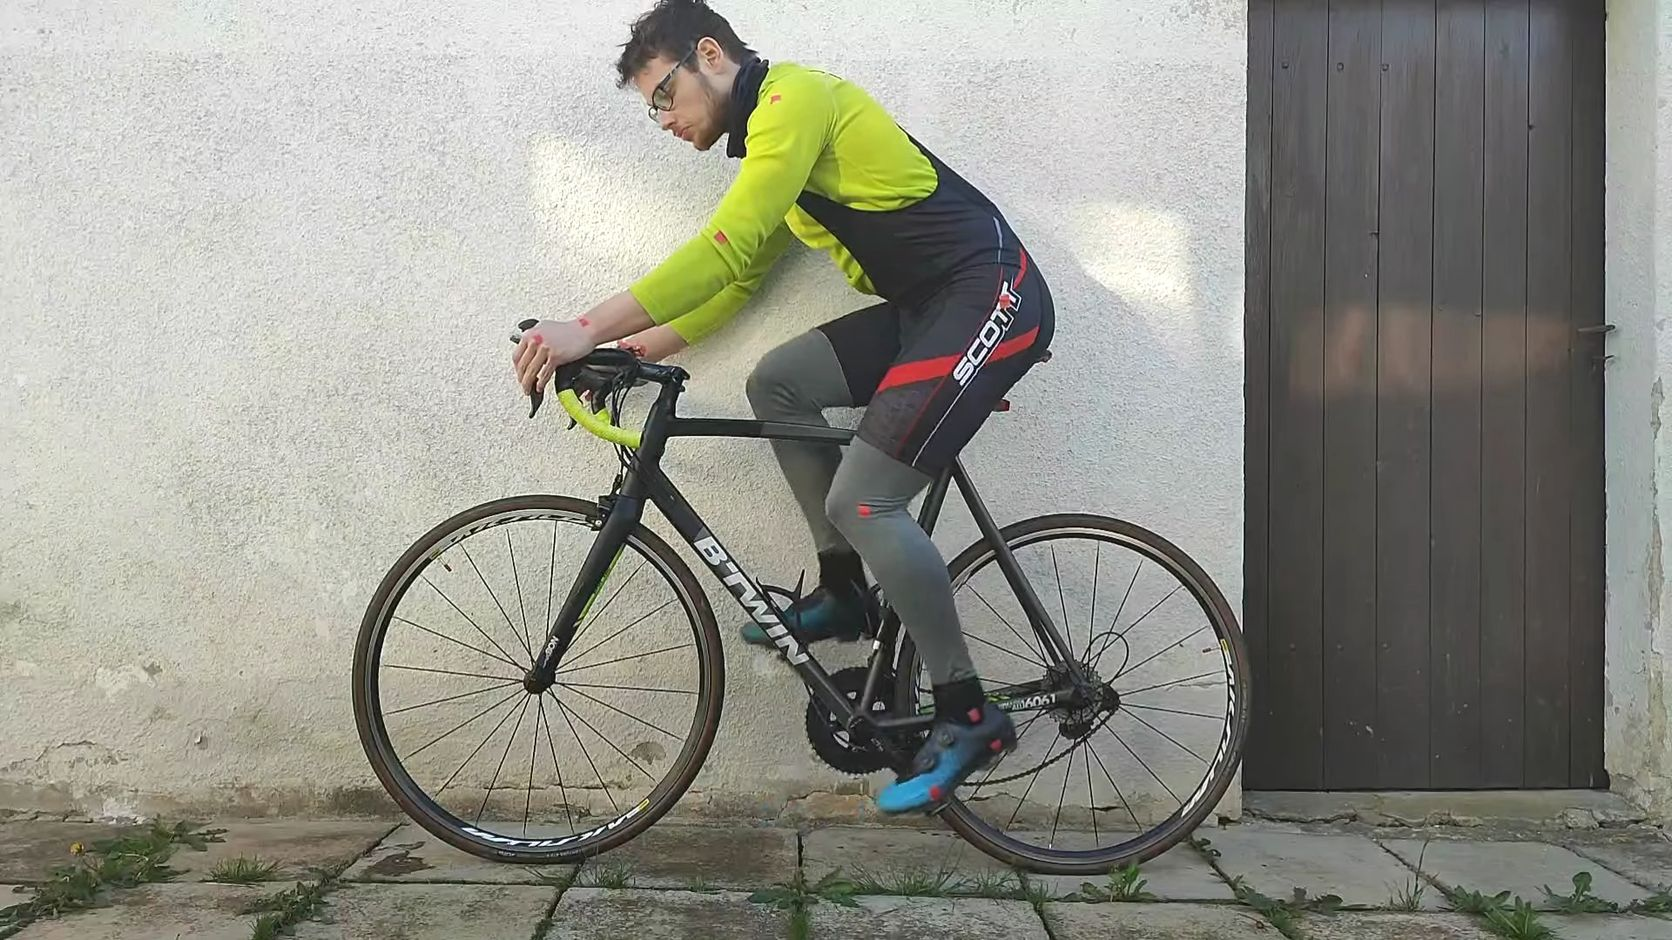
\includegraphics[width=1\linewidth]{obrazky-figures/inpainting_original.jpg}
    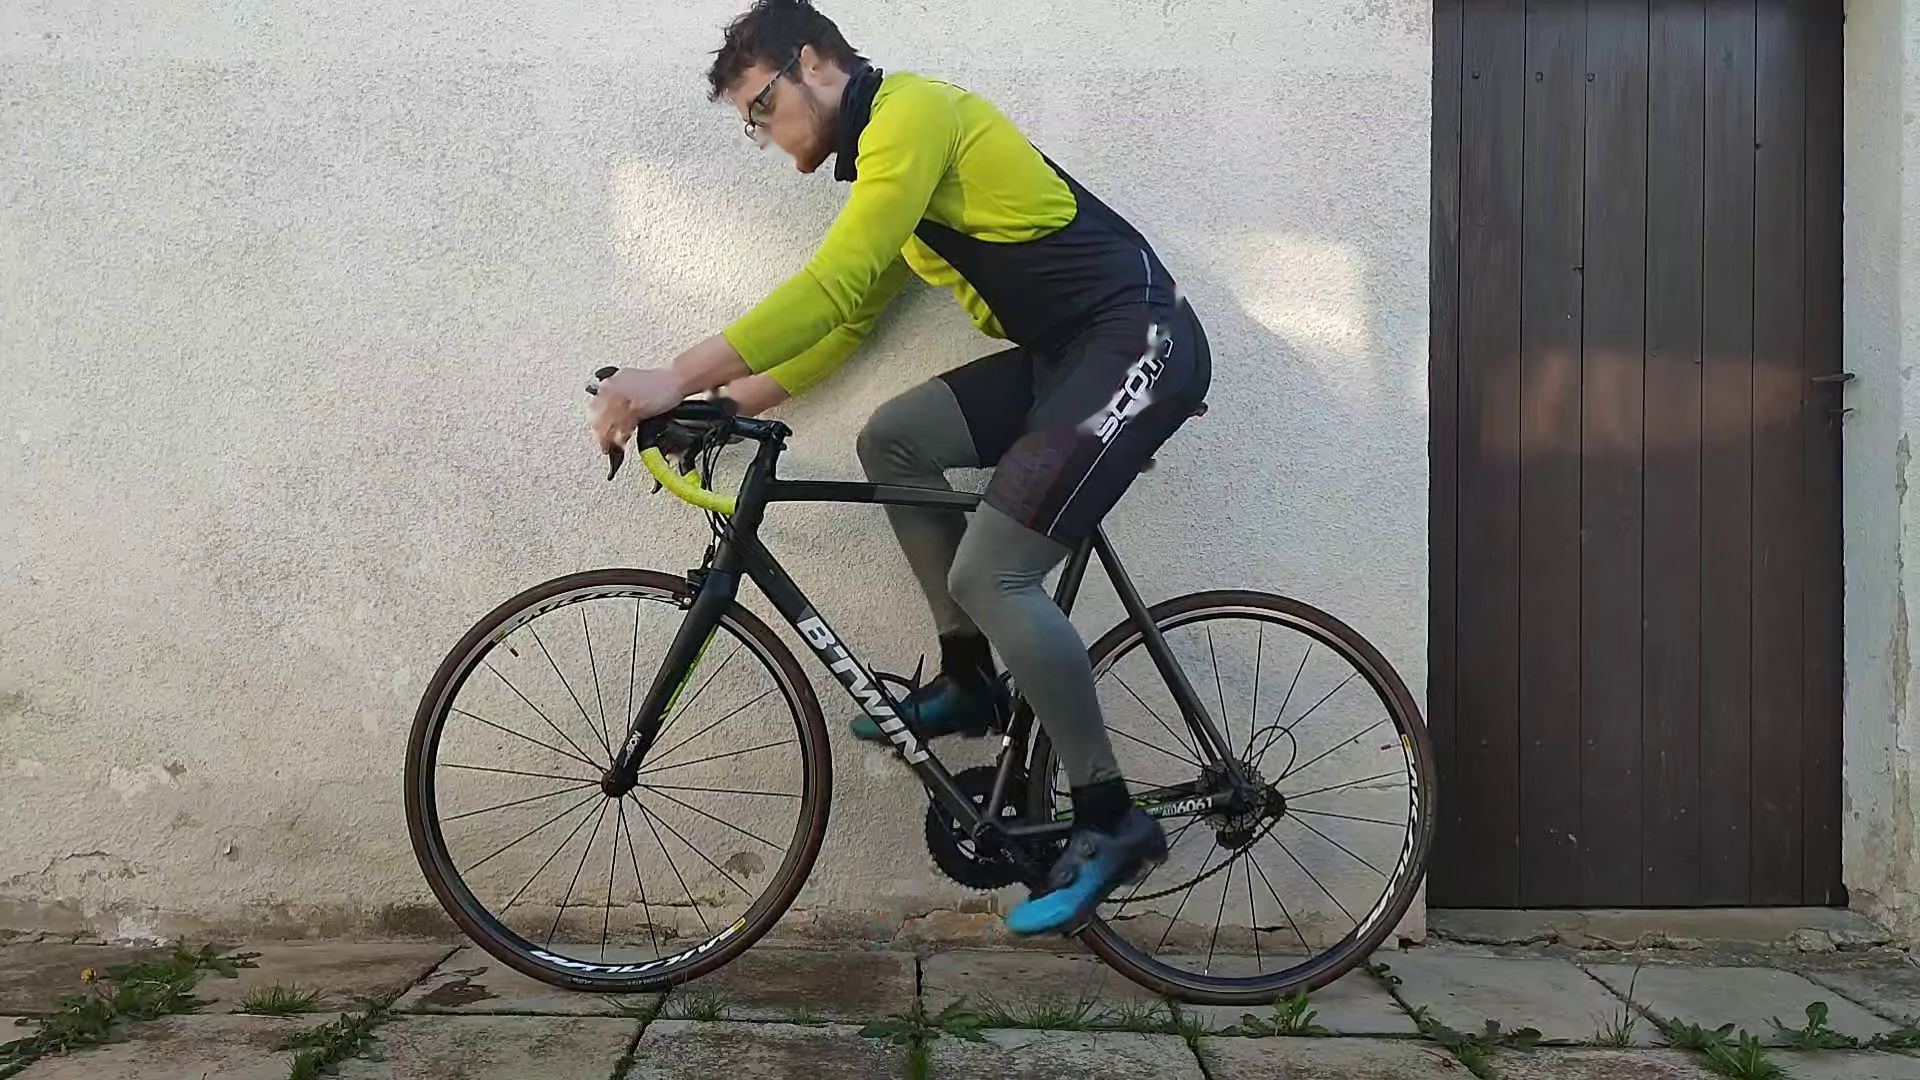
\includegraphics[width=1\linewidth]{obrazky-figures/inpainting.jpg}
    \caption{Example of the removal of the colored markers. The red colored markers are removed from the original image (top) using the Navier-Stokes inpainting algorithm. Most of the markers are removed well, but the algorithm produces blurry results on non-uniform backgrounds (pants with logo) and sometimes inpaints unwanted parts of the image (face), if the mask is not accurate.}
    \label{fig:inpainting}
\end{figure}


\section{Training and Validation Split}
\label{evaluation_dataset}
The extracted frames are split into training and validation sets. Frames from the same video are not split between the training and validation sets. The training set \textbf{1833} frames extracted from \textbf{19} videos and the validation set contains \textbf{476} frames extracted from \textbf{4} videos.





%%%%%%%%%%%%%%%%%%%%%%%%%

\chapter{Fine-Tuning and Evaluation of Pose Estimation Models for Bikefitting}
\label{ch:fine_tuning}

This chapter evaluates the performance of the pose estimation models on side view pose estimation of cyclists. Based on these results the best perfoming model is selected and fine-tuned on the bikefitting dataset. The fine-tuned model is then once again evaluated on the bikefitting dataset and compared with the pre-trained models. This model is then used in the bikefit application. Models are evaluated and fine-tuned on the dataset described in section \ref{ch:dataset}.

The evaluation metrics are described in section \ref{evaluation_metrics}. Initial evaluation of the standard, pre-trained models is done in section \ref{initial_evaluation}. The fine-tuning of the models is described in section \ref{fine_tuning}. The results of the fine-tuned models are shown in section \ref{fine_tuning_results}.

All of the evaluations and training is done using the MMDetection framework \cite{mmdetection} and the MMPose framework \cite{mmpose2020}.

\section{Evaluation Metrics}
\label{evaluation_metrics}
This section describes commonly used metrics for evaluating pose estimation models and their limitations. The Normalized Mean Error (NME) metric, described in section \ref{nme}, is used in the evaluation of the models on the bikefitting dataset.



\subsection{Percentage of Correct Keypoints (PCK)}
Percentage of Correct Keypoints (PCK) is a simple metric that calculates the percentage of keypoints that are within a certain distance from the ground truth keypoints. The distance is normalized by the size of the bounding box of the person. It provides a simple and intuitive measure of the accuracy of the model.

However, for the bikefitting dataset, commonly used thresholds of 0.1 or 0.05 are too big and the models achieved close to 100\% PCK on the validation set. With a lower threshold, the models PCK would swing wildly if the distance between the keypoints and the ground truth keypoints is close to the threshold. This is why the PCK metric is not used in the evaluation of the models on the bikefitting dataset.

\subsection{Object Keypoint Similarity (OKS)}
The Object Keypoint Similarity (OKS) metric is a widely used metric for evaluating pose estimation models. It calculates the similarity between the predicted keypoints and the ground truth keypoints based on the distance between the keypoints and defined variance for each keypoint.

The equation for keypoint similarity is:
$$KS_i = \exp\left(\frac{-d^2_i}{2s^2\sigma^2_i}\right)$$

\begin{description}
    \item[$KS_i$] is the keypoint similarity for keypoint $i$
    \item[$d_i$] is the Euclidean distance between the ground truth and predicted keypoint $i$
    \item[$k_i$] is the variance for keypoint $i$
    \item[$s$] is the scale of the object, $s^2$ is the area of the bounding box of the person
\end{description}

The final OKS is defined as sum of the keypoint similarities of visible keypoints divided by the number of visible keypoints.

It calculates a score between 0 and 1, where 1 means that the predicted keypoints are in the same position as the ground truth keypoints and 0 means that the predicted keypoints are far from the ground truth keypoints. However, it relies on defining the variance for each keypoint, which defines how much can each keypoint vary from the ground truth keypoint. Figure \ref{fig:oks} shows the effect of the variance in the OKS metric for different keypoints. This setting of variance is dataset dependent and can be hard to define for a new dataset. This is why the OKS metric is not used in the evaluation of the models on the bikefitting dataset.

\begin{figure}[htbp]
    \centering
    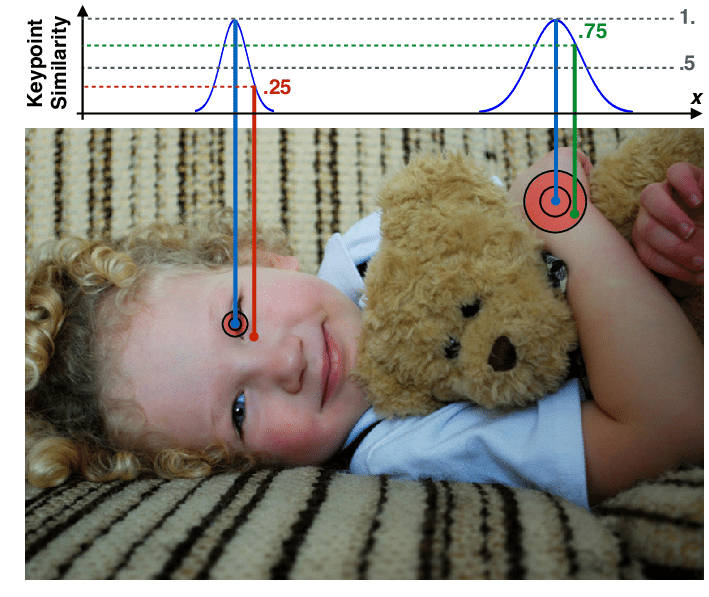
\includegraphics[width=0.7\linewidth]{obrazky-figures/oks.png}
    \caption{Diffent variances in the OKS metric for different keypoints. The keypoint similarity for the eye and wrist keypoints are different, even though the Euclidean distance is the same. Taken from \cite{oks}.}
    \label{fig:oks}
\end{figure}

\subsection{Mean Average Precision (mAP)}

In assessing the performance of pose estimation models, the most widely used metric is the Mean Average Precision (mAP) which is calculated as the average of the precision-recall curve at different thresholds of Object Keypoint Similarity (OKS). This metric is often used in large scale datasets, such as COCO \cite{coco}, where the keypoints of interest are not always visible and therefore are hard to accurately predict. Moreover, these datasets are labeled by multiple annotators, which can lead to inconsistencies in the annotations.
This metric intuitively tells us how many keypoints are in some proximity to the ground truth keypoints. However, in the case of the bikefitting dataset, where only few well visible keypoints are of interest, the mAP metric may not be the most suitable for evaluation, since all of the keypoints should be in close proximity to the ground truth keypoints and we are more interested in the exact error of the keypoints.


\subsection{Normalized Mean Error (NME)}
\label{nme}
As was discussed in the previous sections, the commonly used metrics for evaluating pose estimation models, such as PCK, OKS, and mAP, may not be suitable for the bikefitting dataset. This is why a simple Normalized Mean Error (NME) metric is used for evaluation of the models on the bikefitting dataset.


Normalized Mean Error (NME) is calculated by obtaining the Euclidean distance between the predicted keypoints and the ground truth keypoints, and then normalizing this distance with respect to the average bounding box dimension. The normalization is done to account for the scale of the video. It is then expressed as a percentage for better interpretability. The formula for NME is as follows:

$$ \text{NME}_i (\%)= \frac{d_i}{\frac{{s.w} + {s.h}}{2}} \cdot 100 $$

Where:
\begin{description}
    \item[$\text{NME}_i$:] is the Normalized Mean Error for the $i$-th keypoint, expressed as a percentage of the average bounding box dimension
    \item[$d_i$:] is the Euclidean distance between the ground truth and predicted keypoint $i$
    \item[$s.w$:] is the width of the bounding box of the person
    \item[$s.h$:] is the height of the bounding box of the person
\end{description}

The NME for keypoint $i$ is then averaged over all keypoints to obtain the NME for a single frame. The final NME is then calculated over all frames in the dataset. NME offers easy to interpret results, with a lower value indicating a more accurate prediction.

\section{Initial Evaluation of Pre-Trained Models}
\label{initial_evaluation}
This section evaluates the performance of the pre-trained pose estimation models on the bikefitting dataset. This is done, since there can be a significant difference in the performance of the models on COCO dataset and the bikefitting dataset. The models are evaluated using the NME metric, described in section \ref{evaluation_metrics}.

The models are evaluated using the MMPose framework \cite{mmpose2020}, with the Inferencer API and the PyTorch backend. Topdown models (models that require inputs cropped to the bounding box of the person) use the RTMDet-nano model \cite{rtmdet} from the MMDetetection framework \cite{mmdetection} for person detection.

As was described in chapter \ref{ch:pose_estimation}, some models predict more keypoints than others. Most of the models are trained to predict 17 keypoints, as defined in the COCO dataset. The RTMPose, which are also trained on other datasets, inlcuding Halpe26, predict 26 keypoints. The WholeBody models predict 133 keypoints. The keypoints that are not needed for the evaluation are ignored. Since no models predict the fifth metatarsal of the foot, which is a crucial point for bikefitting, the small toe landmark is used instead.

\subsection{6 Keypoint Evaluation}

At first the models are evaluated using only the 6 keypoints that are both in the COCO dataset and the bikefitting dataset (camera facing ankle, knee, hip, shoulder, elbow and wrist). The results are shown in table \ref{tab:evaluation_results_all}. The best results are achieved by the RTMPose-m 384x288 model, but most of the bigger RTMPose models outperform the other models. This is in contrast to the results on the COCO dataset, where HRNet-W32 model performed similarly to the bigger RTMPose models. The relative decrease in performance of the HRNet-W32 model is probably caused by the fact that it was trained only on the COCO dataset, while the RTMPose models were trained on multiple datasets and are more robust to different poses and camera angles.




\begin{table}[htbp]
    \begin{tabular}{l cccc}
        \toprule
        Architecture          & Input Size & Trained On     & Keypoints & NME (\%)      \\
        \midrule
        RTMPose-m             & 384x288    & Body8          & 17        & \textbf{2.12} \\
        RTMPose-l             & 384x288    & Body8          & 17        & 2.13          \\
        RTMPose-m             & 256x192    & Body8          & 17        & 2.22          \\
        RTMPose-m             & 384x288    & Body8-Halpe26  & 26        & 2.23          \\
        RTMPose-l             & 256x192    & Body8          & 17        & 2.27          \\
        RTMPose-m             & 256x192    & Body8-Halpe26  & 26        & 2.28          \\
        HRNet-w32             & 256x192    & COCO           & 17        & 2.34          \\
        RTMPose-l             & 384x288    & Body8-Halpe26  & 26        & 2.42          \\
        RTMPose-l             & 256x192    & Body8-Halpe26  & 26        & 2.43          \\
        RTMPose-s             & 256x192    & Body8          & 17        & 2.52          \\
        RTMPose-s             & 256x192    & Body8-Halpe26  & 26        & 2.56          \\
        RTMPose-l             & 256x192    & COCO-WholeBody & 133       & 2.59          \\
        RTMPose-m             & 256x192    & COCO-WholeBody & 133       & 2.61          \\
        RTMPose-t             & 256x192    & Body8-Halpe26  & 26        & 2.68          \\
        SimCC\_ViPNAS-MBNetv3 & 256x192    & COCO           & 17        & 2.70          \\
        RTMPose-t             & 256x192    & Body8          & 17        & 2.70          \\
        Yoloxpose\_m          & 640x640    & COCO           & 17        & 2.74          \\
        \bottomrule
    \end{tabular}
    \caption{Evaluation results on the custom bike fitting dataset, using only 6 keypoints most important to bikefitting (camera facing ankle, knee, hip, shoulder, elbow and wrist). The results are sorted by the Normalized Mean Error, defined in section \ref{nme}. It is an average distance between the predicted keypoints and the ground truth keypoints, normalized by the average bounding box dimension, expressed as a percentage. The larger RTMPose models trained on the Body8 datasets outperform the other models.}
    \label{tab:evaluation_results_all}

\end{table}

The best model achieves a mean NME of \textbf{2.12\%}. This means that the average distance between the predicted keypoints and the ground truth keypoints is \textbf{2.12\%} of the average bounding box dimension.

The good results of the RTMPose models are not surprising, since they were trained on multiple datasets, while the other models were trained only on the COCO dataset. The RTMPose models trained on the Body8 dataset perform slightly better than those trained on the Body8-Halpe26 dataset, which were trained to predict 26 keypoints. However, the models trained on COCO-WholeBody dataset perform significantly worse, this is probably because the WholeBody dataset is much smaller than the Body8 and standard COCO datasets.

The other lightweight models (YOLOX-Pose and ViPNAS-MobileNetV3) perform significantly worse than the RTMPose models. The YOLOX-Pose model is the worst performing model, with a mean NME of \textbf{2.74\%}. The ViPNAS-MobileNetV3 model performs slightly better, but still worse than even the tiny RTMPose model.

Overall, we can see few unsurprising results. Models that are larger, or trained on multiple datasets, perform better than the smaller models trained only on the COCO dataset. It is interesting though, that there is not a huge difference between the large and medium RTMPose models, but there is a clear advantage to RTMPose models with larger input size. This is probably because the larger input size allows the model to capture more details in the image.

\subsection{8 Keypoint Evaluation}
The models which also output heel and foot fingers keypoints are evaluated on all of the 8 keypoints present in the bikefitting dataset. Meaning the camera facing fifth foot metatarsal and heel are also evaluated. The results are shown in table \ref{tab:evaluation_results_wholebody}. We can see, that the Normalized Mean Error (NME) for the foot and heel keypoints is much higher than for the other keypoints. This highlights the difficulty of predicting the foot and heel keypoints, as these keypoints are less represented in the training datasets. The models that output the WholeBody keypoints perform slightly worse than the models that only output Halpe26 keypoints, but the difference is smaller than when comparing only the 6 keypoints. What is surprising, is that the COCO-WholeBody models perform better than the Halpe26 on the foot and heel keypoints. This can be because the COCO-WholeBody dataset keypoints may match the foot and heel keypoints defined in the bikefitting better than the Halpe26 dataset. However, overall the best performing models are still the RTMPose models trained on the Body8 dataset, with the RTMPose-m 384x288 model achieving the best results with a mean NME of \textbf{2.49\%}.

\begin{table}[htbp]
    \setlength{\tabcolsep}{4pt}
    \centering
    \begin{tabular}{l cccccc}
        \toprule
        Architecture & Input Size & Trained On     & Keypoints & Foot (\%)     & Heel (\%)     & Mean (\%)     \\
        \midrule
        RTMPose-m    & 384x288    & Body8-Halpe26  & 26        & 3.45          & 3.40          & \textbf{2.49} \\
        RTMPose-m    & 256x192    & Body8-Halpe26  & 26        & 3.29          & 3.62          & 2.54          \\
        RTMPose-l    & 256x192    & Body8-Halpe26  & 26        & 3.56          & 3.21          & 2.64          \\
        RTMPose-l    & 384x288    & Body8-Halpe26  & 26        & 3.48          & 3.58          & 2.67          \\
        RTMPose-l    & 256x192    & COCO-WholeBody & 133       & \textbf{2.55} & 3.45          & 2.68          \\
        RTMPose-s    & 256x192    & Body8-Halpe26  & 26        & 3.14          & 3.52          & 2.73          \\
        RTMPose-m    & 256x192    & COCO-WholeBody & 133       & 3.25          & \textbf{3.15} & 2.74          \\
        RTMPose-t    & 256x192    & Body8-Halpe26  & 26        & 4.21          & 3.20          & 2.91          \\
        \bottomrule
    \end{tabular}
    \caption{Evaluation results for the models with extended keypoint set on the custom bike fitting dataset, including the heel and foot landmarks. Results for the other keypoints can be found in table \ref{tab:evaluation_results_coco}. Foot column shows the Normalized Mean Error (NME) for the foot landmark, Heel column shows the NME for the heel landmark and Mean column shows the average NME for all of the 8 keypoints present in the bikefitting dataset. The values are represented as a percentage of the average bounding box dimension for a given frame. Details of the NME metric are described in section \ref{nme}.}
    \label{tab:evaluation_results_wholebody}

\end{table}

Figure \ref{fig:evaluation_examples} shows example predictions of the models on the bikefitting dataset. The RTMPose-m 384x288 Body8 model achieves the best results. The RTMPose-m 384x288 Body8-Halpe model also achieves good results, and also predicts the heel and foot keypoints. The RTMPose-l 256x192 COCO-WholeBody model performs much worse on the foot and heel keypoints. The accuracy of the SimCC\_ViPNAS-MBNetv3 is also worse than the RTMPose models.

\def\imgwidth{0.45\textwidth}
\def\smallimgwidth{0.9\textwidth}

\begin{figure}[htbp]
    \centering
    \begin{subfigure}[b]{\imgwidth}
        \centering

        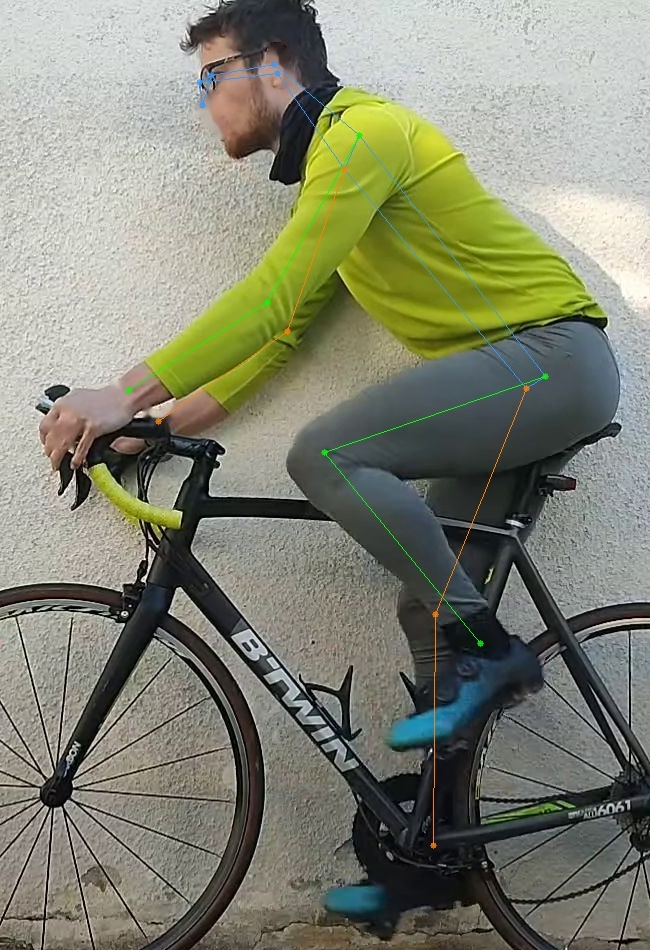
\includegraphics[width=\smallimgwidth]{obrazky-figures/rtmpose-m_8xb256-420e_body8-384x288_zlute_196_crop.jpg}
        \caption{RTMPose-m 384x288 Body8}

    \end{subfigure}
    \hfill
    \begin{subfigure}[b]{\imgwidth}
        \centering

        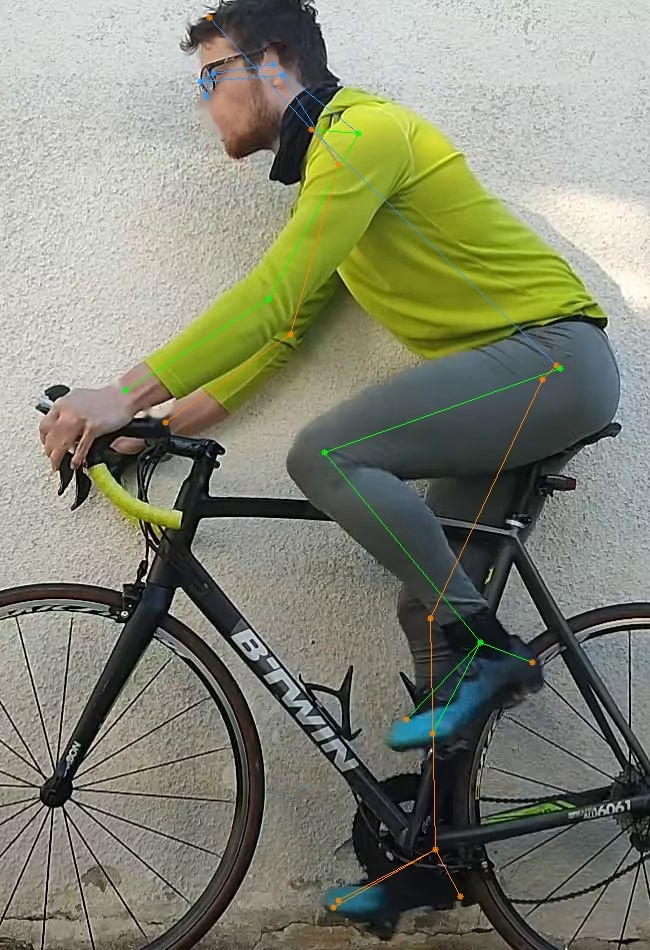
\includegraphics[width=\smallimgwidth]{obrazky-figures/rtmpose-m_8xb512-700e_body8-halpe26-384x288_zlute_196_crop.jpg}
        \caption{RTMPose-m 384x288 Body8-Halpe}
    \end{subfigure}
    \hfill
    \par\bigskip

    \begin{subfigure}[b]{\imgwidth}
        \centering

        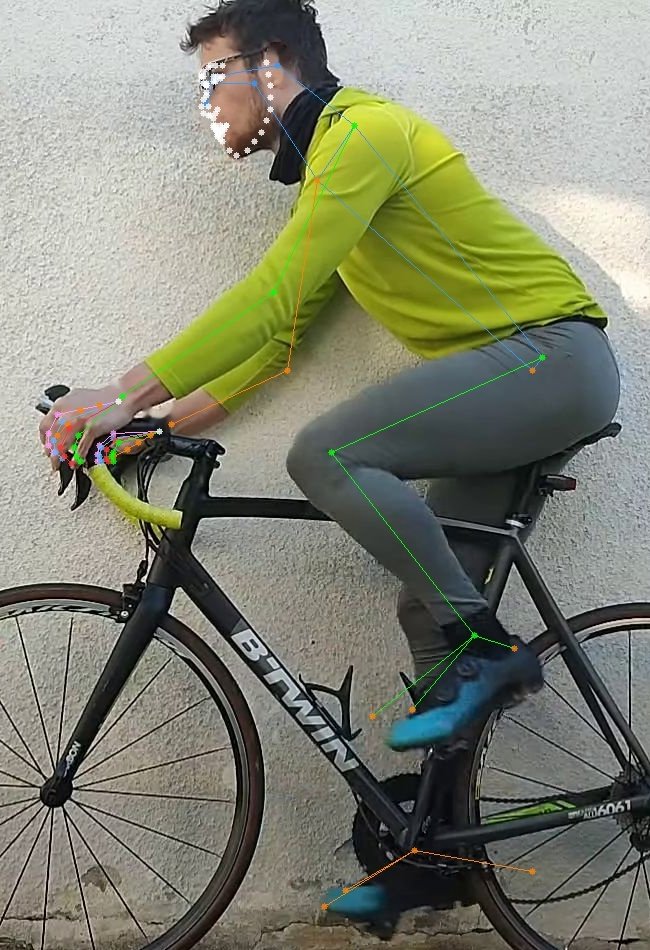
\includegraphics[width=\smallimgwidth]{obrazky-figures/rtmpose-l_8xb64-270e_coco-wholebody-256x192_zlute_196_crop.jpg}
        \caption{RTMPose-l 256x192 COCO-WholeBody}


    \end{subfigure}
    \hfill
    \begin{subfigure}[b]{\imgwidth}
        \centering

        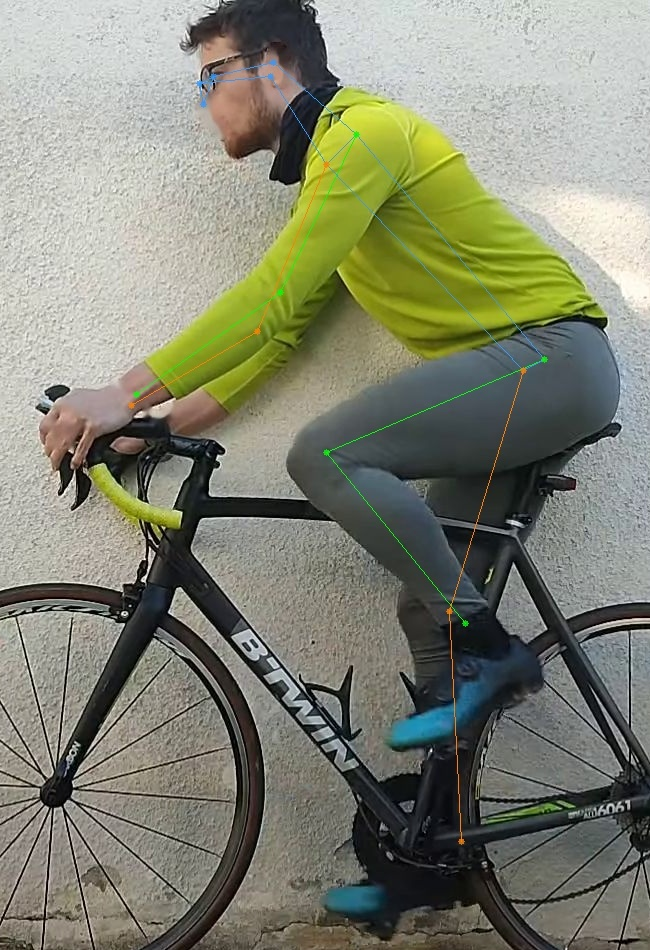
\includegraphics[width=\smallimgwidth]{obrazky-figures/simcc_vipnas-mbv3_8xb64-210e_coco-256x192_zlute_196_crop.jpg}
        \caption{SimCC\_ViPNAS-MBNetv3}


    \end{subfigure}
    \caption{
        Example predictions of the models on the bikefitting dataset. Models (a) and (d) predict standard 17 COCO keypoints, while model (b) predicts 26 Halpe keypoints and model (c) predicts 133 WholeBody keypoints. The RTMPose-m 384x288 Body8 model (a) achieves the best results.}
    \label{fig:evaluation_examples}

\end{figure}

The RTMPose models show good results on the bikefitting dataset. However, the accuracy on the foot and heel keypoints is still not satisfactory even for the largest models trained on the Body8-Halpe26 dataset. The results are even worse for the models trained on the COCO-WholeBody dataset. To improve the accuracy of the models on the foot and heel keypoints, the models need to be fine-tuned on the bikefitting dataset. The details of the fine-tuning are described in the next section.

\section{Fine-Tuning On Custom Bikefit Dataset}
\label{fine_tuning}
For the fine-tuning, the RTMPose-m 256x192 Body8-Halpe26, RTMPose-l 256x192 Body8-Halpe26 and RTMPose-m 384x288 Body8-Halpe26 models are selected. These models are selected, because they achieved good results on the bikefitting dataset, predict the heel and foot keypoints and are still relatively fast. The models are fine-tuned on the bikefitting dataset using the MMPose framework \cite{mmpose2020}.

To train a model using the MMPose framework, the model needs to have a custom config file for the dataset. The config file contains the paths to the dataset, the model architecture, the optimizer, the learning rate scheduler and other hyperparameters. The original config files for the RTMPose models were used as a starting point and modified to use the bikefitting dataset different hyperparameters and evaluation metrics.

Custom datasets in MMPose are easiest to define using the COCO format. The dataset is defined in a JSON file, which contains the paths to the images, the annotations and the categories. The annotations contain the bounding box of the person and the keypoints. The keypoints are defined as a list of x and y coordinates and a visibility flag. The visibility flag is set to 2 if the keypoint is not visible, 1 if the keypoint is occluded and 0 if the keypoint is visible. MMPose internally uses only annotated keypoints (visibility flag 2 or 1) for training and evaluation and discards keypoints with visibility flag 0. The training set has all of the keypoints defined as annotated (visibility flags 1 or 2), so the models are trained on all of the keypoints. This ensures that the models do not unlearn the other keypoints. The validation set has only the 8 keypoints annotated by colored markers defined as annotated, so the models are evaluated only on these keypoints.

\subsection{Training Procedure}
The RTMPose models originally used the AdamW \cite{adamw} optimizer with base learning rate of 4e-3, linear warmup learning rate scheduler for first 1000 iterations and cosine annealing learning rate scheduler. The models were in total trained for 700 epochs with training batch size of 512. These are tuned for a large scale dataset like COCO. For the bikefitting dataset, smaller learning rate and batch size are used. The models are trained with the AdamW optimizer with base learning rate of 5e-4, no learning rate schedulerers were used as this slowed down the training. The batch size was reduced to 16, as this sped up the training significantly. The models were trained for 130 iterations, which corresponds to 1 epoch on the bikefitting dataset. Using larger batch sizes of 32 and 64 resulted in much slower training, where the models needed 5-10 epochs of training and still achieved worse results then when using batch size of 16. The models were fast enough to be trained on an single Intel i7-7500U CPU.


Figure \ref{fig:fine_tuning_loss} shows the loss of the models during the fine-tuning. The RTMPose large and medium models with 256x192 input size achieve basically the same loss throughout the training. The RTMPose-m 384x288 model has significantly lower loss than the other models throughout the whole training. Since its validation results are on par with the 256x192 models (as discussed in the next section), it is probably because different parameters are used to construct the ground truth heatmaps for the 384x288 model, which results in lower loss. Overall the loss of the models is decreasing throughout the training, at first rapidl and then about step 60 more slowly. However, experiments showed that while the loss is not decreasing very fast, the results are still improving.
% TODO: add more details about the training procedure
\begin{figure}

    \centering
    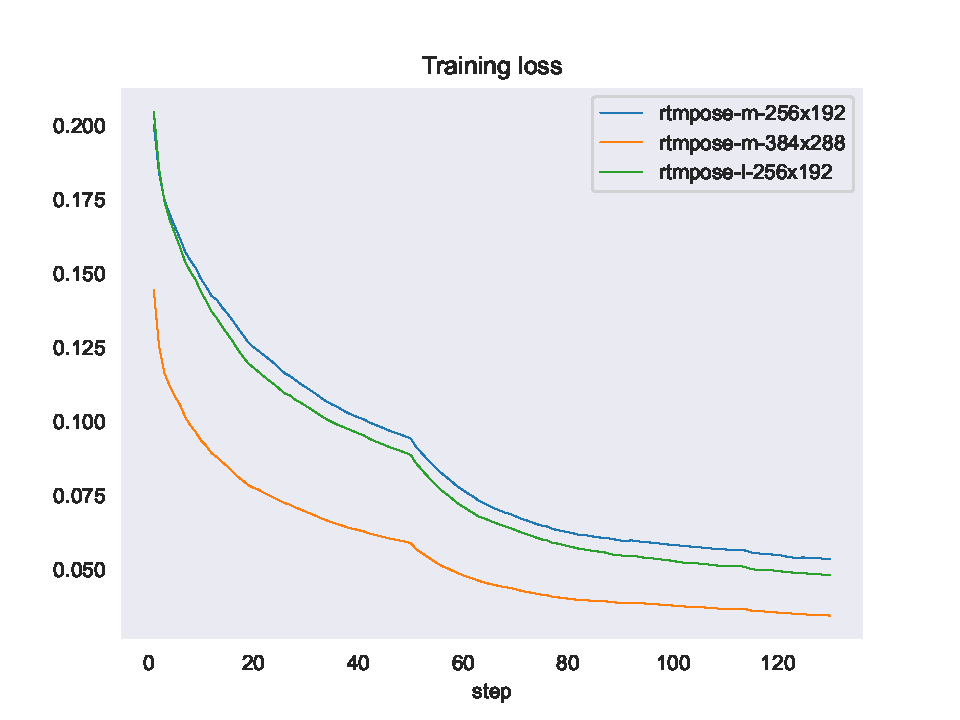
\includegraphics[width=1\linewidth]{obrazky-figures/loss.pdf}

    \caption{Loss of the RTMPose models during fine-tuning on the bikefitting dataset. The models were trained for 130 iterations, which corresponds to 1 epoch on the bikefitting dataset. For optimization, AdamW optimizer with base learning rate of 5e-4 and batch size of 16.}
    \label{fig:fine_tuning_loss}
\end{figure}


\section{Evaluation Of Fine-Tuned Models}
\label{fine_tuning_results}
Table \ref{tab:finetune_results} shows the results of the fine-tuned models on the bikefitting dataset. The models are evaluated using the NME metric, described in section \ref{evaluation_metrics}. All of the fine-tuned models achieve significantly better results than the pre-trained models. Despite the differences in the performance of medium and large pre-trained models, the fine-tuned models achieve similar results. The best results are achieved by the RTMPose-m 384x288 model, which achieves a mean NME of \textbf{1.50\%}, but the other fine-tuned models achieve very similar results. The fine-tuned models achieve a significant improvement in the accuracy of the foot and heel keypoints. The foot and heel keypoints are still the most difficult to predict, but the fine-tuned models achieve much better results than the pre-trained models. Because there is not a significant difference in the performance of the fine-tuned models, the RTMPose-m 256x192 model is selected for the bikefit application, as it is the smallest and fastest model that achieves good results.

\def\imgwidth{0.48\textwidth}
\def\smallimgwidth{1.0\textwidth}

\begin{table}[htbp]
    \setlength{\tabcolsep}{4pt}
    \centering
    \begin{tabular}{l cccccc}
        \toprule
        Architecture & Input Size & Trained On      & Keypoints & Foot (\%)     & Heel (\%)     & Mean (\%)     \\
        \midrule
        RTMPose-m    & 384x288    & Bikefit dataset & 26        & \textbf{1.25} & 2.11          & \textbf{1.50} \\
        RTMPose-m    & 256x192    & Bikefit dataset & 26        & 1.45          & 1.99          & 1.51          \\
        RTMPose-l    & 256x192    & Bikefit dataset & 26        & 1.26          & \textbf{1.94} & 1.52          \\
        RTMPose-m    & 384x288    & Body8-Halpe26   & 26        & 3.45          & 3.40          & 2.49          \\
        RTMPose-m    & 256x192    & Body8-Halpe26   & 26        & 3.29          & 3.62          & 2.54          \\
        RTMPose-l    & 256x192    & Body8-Halpe26   & 26        & 3.56          & 3.21          & 2.64          \\
        \bottomrule
    \end{tabular}
    \caption{Evaluation results for the fine-tuned models on the custom bike fitting dataset. The models are fine-tuned on the bikefitting dataset for 130 iterations. The results are sorted by the Normalized Mean Error, defined in section \ref{nme}. It is an average distance between the predicted keypoints and the ground truth keypoints, normalized by the average bounding box dimension, expressed as a percentage. All of the fine-tuned models achieve significantly better results than the pre-trained models.}
    \label{tab:finetune_results}

\end{table}

Figure \ref{fig:trained_examples} shows example predictions of the RTMPose-m 256x192 model before and after fine-tuning. The fine-tuned model achieves much better results on the foot and heel keypoints. It also shifts the knee and shoulder keypoints more closely to the location which are used for example in the Retul bikefitting system. However, it also shifts the hip keypoint closer to the knee keypoint, which is not desirable. Similarly, the wrist keypoint is now no longer predicted on the center of rotation of the wrist joint, but more upwards. These changes are probably caused by misplacement of the colored markers, which is especially hard to avoid when muliple poses and camera angles are present in the dataset. Nevertheless, the fine-tuned model overall achieves better results than the pre-trained model and is used in the bikefit application.
\begin{figure}[htbp]
    \centering
    \begin{subfigure}[t]{\imgwidth}
        \centering

        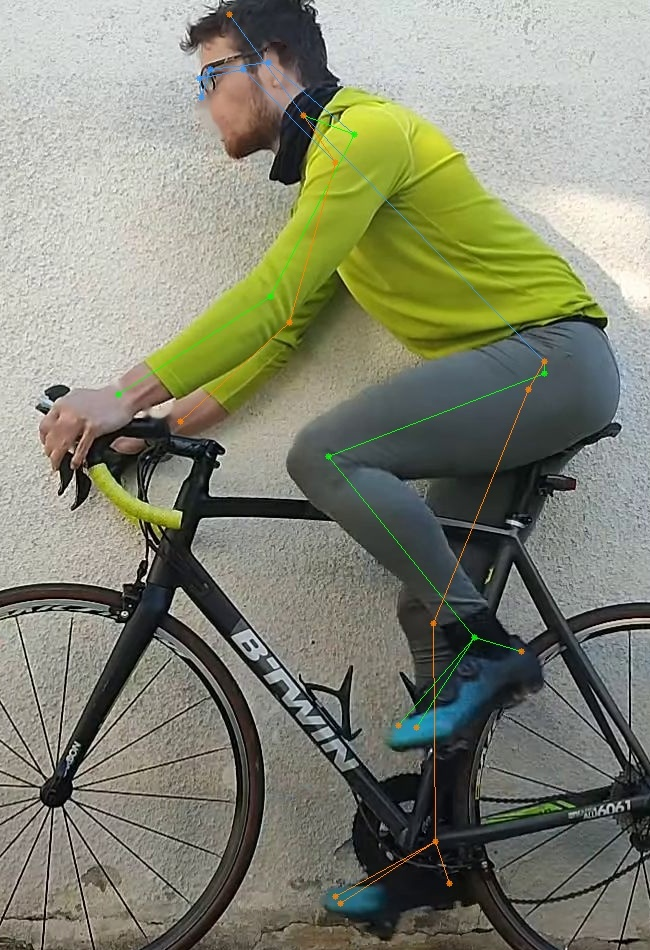
\includegraphics[width=\smallimgwidth]{obrazky-figures/rtmpose-m_8xb512-700e_body8-halpe26-256x192_zlute_196_crop.jpg}
        \caption{RTMPose-m 256x192 Body8-Halpe26}

    \end{subfigure}
    \hfill
    \begin{subfigure}[t]{\imgwidth}
        \centering

        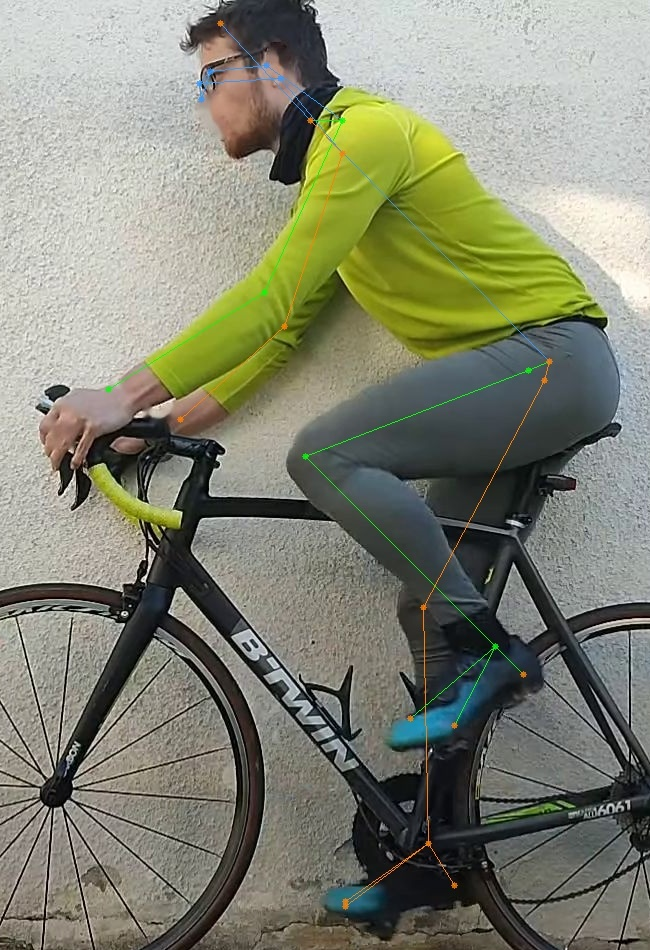
\includegraphics[width=\smallimgwidth]{obrazky-figures/rtmpose-m-256x192_trainedzlute_196_crop.jpg}
        \caption{RTMPose-m 256x192 Body8-Halpe26 Fine-Tuned}
    \end{subfigure}
    \caption{
        Example predictions of the RTMPose-m 256x192 model before and after fine-tuning on the bikefitting dataset. The fine-tuned model achieves much better results on the foot and heel keypoints, but also undesirably shifts the hip and wrist keypoints, probably due to misplacement of the colored markers.}
    \label{fig:trained_examples}
\end{figure}

%%%%%%%%%%%%%%%%%%%%%%%%%%%%%%%%%%%%%%

\chapter{Bikefit Web Application}
\label{ch:bikefit_application}

This chapter describes the web application for bike fitting. Implementing the application as a web application has several advantages over implementing it as a mobile or desktop application. The web application can be used on any device with a web browser. This allows the application to be used on mobile devices, tablets, laptops and desktop computers. The user also does not need to download and install anything.

Most web applications are implemented using the client-server architecture with the video processing and other more complicated tasks (such as pose estimation) being performed on the server. This has several disadvantages. The server needs to be powerful enough to handle the load of multiple users. This can be quite expensive for heavy models and a lot of users. The user data also needs to be sent to the server, which means the user needs to be online when using the application and the users can be concerned about their privacy.

To avoid these disadvantages, all of the logic of the application (including video processing, keypoint estimation and generation of the suggestions) is implemented on the client side.

The application is implemented using the Svelte framework\footnote{\url{https://svelte.dev/}} . Svelte is a component framework similar to React\footnote{\url{https://react.dev/}} or Vue\footnote{\url{https://vuejs.org/}}. It is used to create reactive user interfaces. Svelte compiles the application to vanilla JavaScript, which means the application does not need to include a large framework library. This makes the application smaller and faster. Svelte also has a built-in state management system, which is used to store the application state.

User can upload a video of the cyclist from side view. The video is processed frame by frame by the pose estimation model. The keypoint predictions are then used to compute the joint angles. The joint angles are used to generate the suggestions for the bike fit. The suggestions are displayed to the user. The application from the user perspective is more thoroughly described in section \ref{application_structure}.

The following sections describe the implementation of the application in more detail. To process the video frame by frame, the application uses the WebCodecs API. The details of the implementation are described in section \ref{video_upload_and_processing}. To estimate the keypoint positions, the application uses the RTMPose-m Body8-Halpe26 pose estimation model, which was fine-tuned on the bikefitting dataset. The details of the deployment and implementation are described in section \ref{pose_estimation}. From the keypoint positions, the application computes various joint angles and measurements. The details of the implementation are described in section \ref{computing_joint_angles}. The application then uses the computed joint angles and measurements to generate the suggestions for the bike fit. The details of the implementation are described in section \ref{generating_suggestions}. Lastly, to play the video with the keypoint predictions overlaid on the video, a custom canvas based video player is implemented. The details of the implementation are described in section \ref{video_player}.
\section{User Interface}
\label{application_structure}
From the user's perspective, the application consists of three main steps: video upload, select fit goals and examine suggestions. The user is guided through these steps by a wizard-like interface. The following sections describe each of the steps in more detail.


\subsection{Video Upload} The first step is the video upload. The user is prompted to upload a video of the cyclist from the side view. The user can also choose to use a demo video for testing the application. After the video is uploaded, the user can proceed to the next step. Figure \ref{fig:step1} shows the first step of the application.

\begin{figure}[htbp]
    \centering
    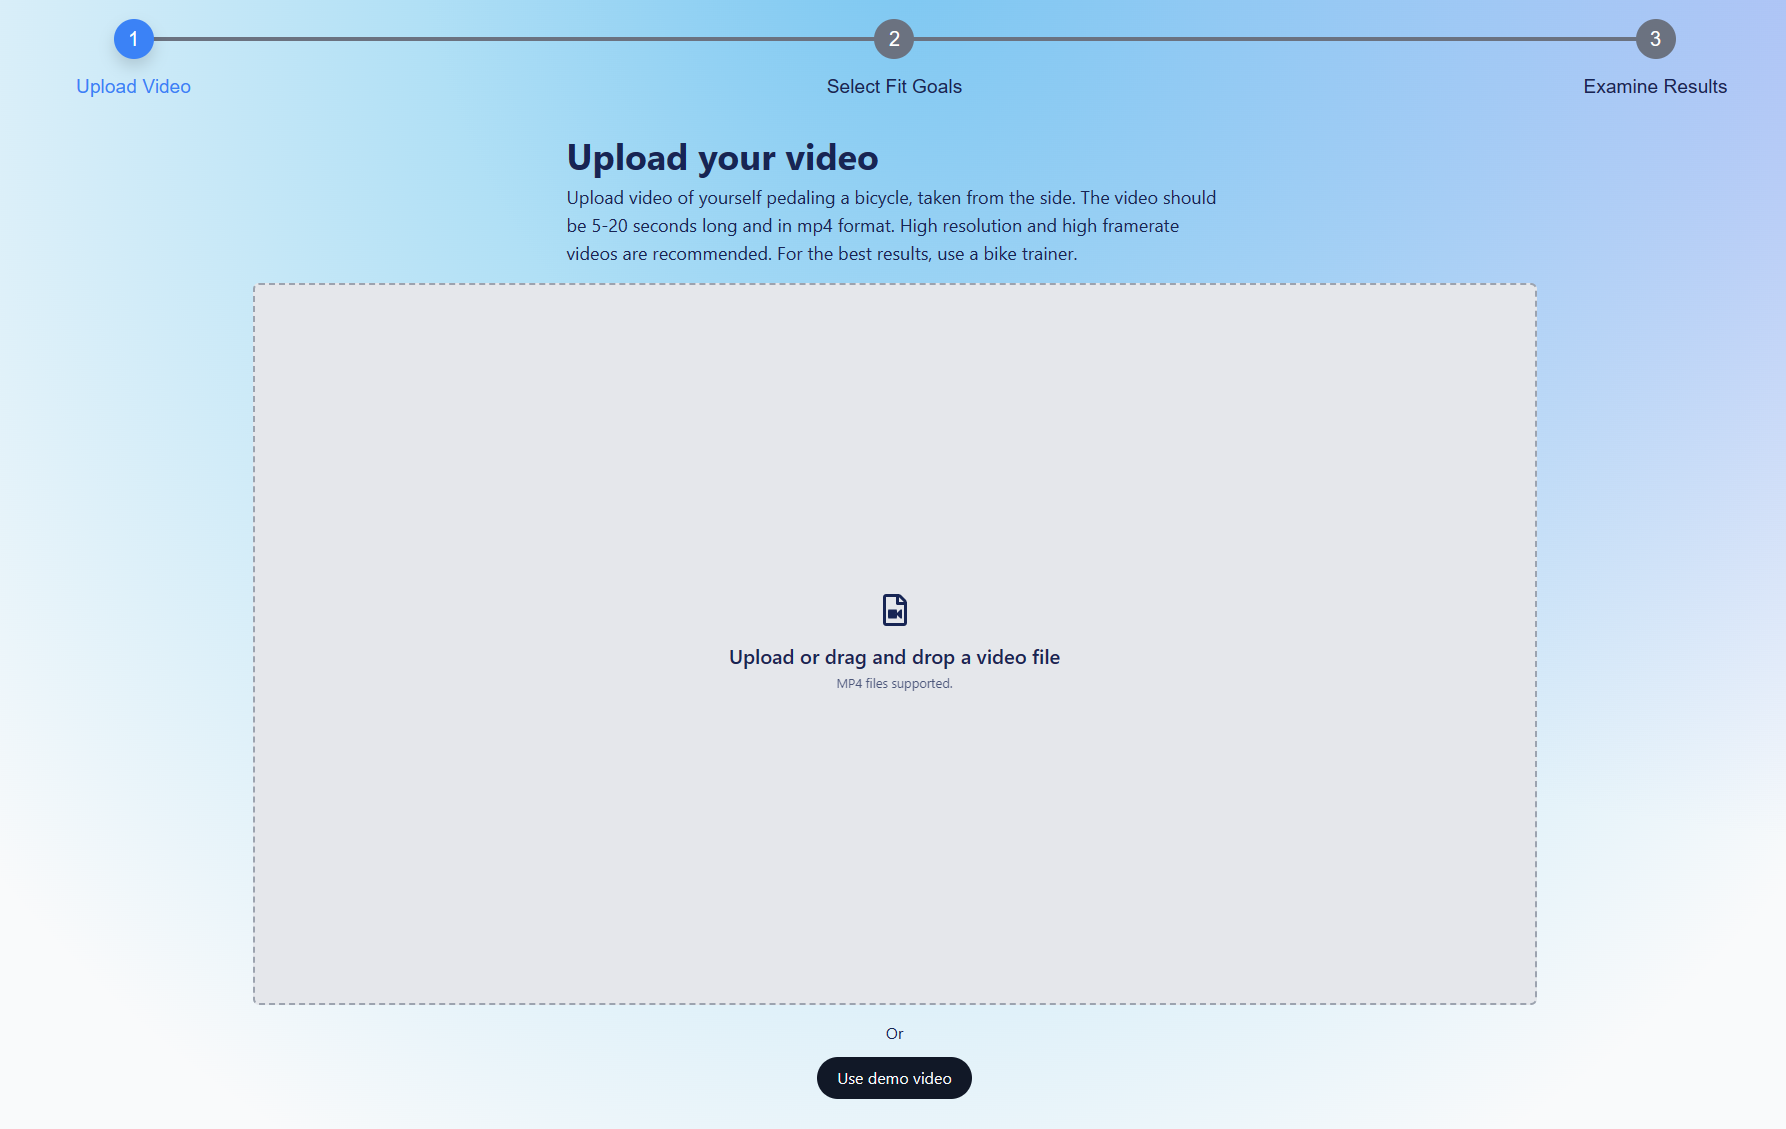
\includegraphics[width=\textwidth]{obrazky-figures/step1-crop.png}
    \caption{The first step of the bikefit application. The user is prompted to upload a video of the cyclist from the side view. The user can also choose to use a demo video for testing the application. After the video is uploaded, the user can proceed to the next step.}
    \label{fig:step1}
\end{figure}

\subsection{Select Fit Goals}

On the second step, shown in figure \ref{fig:step2}, the user can review and play the uploaded video and is asked to select the type of the bike (road, gravel and mountain bike) and the fit goals (comfort, performance, balanced). These fit goals and the type of the bike are used to adjust the suggestions for the bike fit. After the fit goals are selected, the user can process the video by the pose estimation model by clicking on the blue "Process Video" button on the right.

\begin{figure}[htbp]
    \centering
    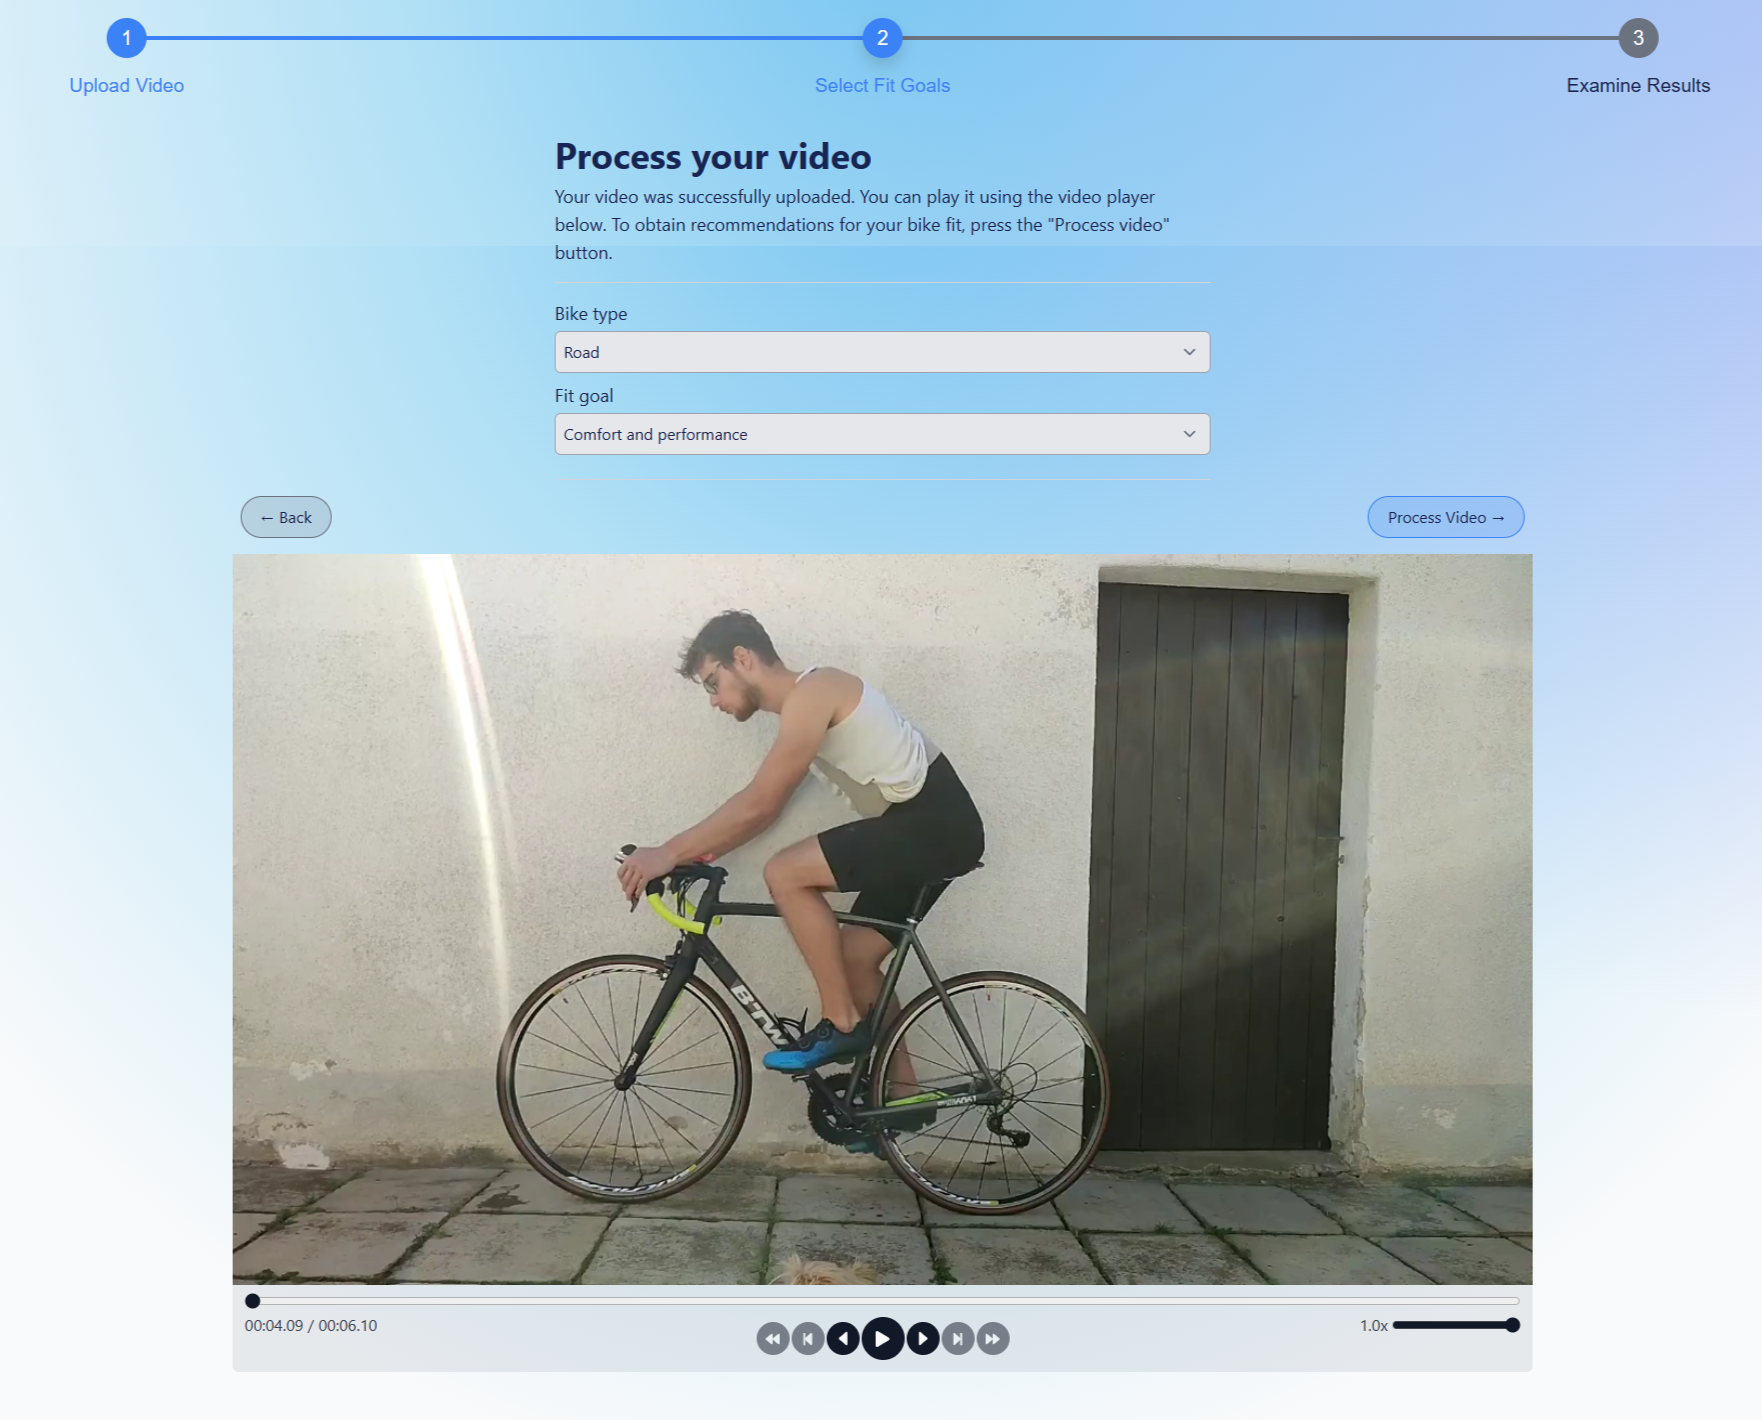
\includegraphics[width=\textwidth]{obrazky-figures/step2-crop.png}
    \caption{The second step of the bikefit application. The user can review and play the uploaded video and is asked to select the type of the bike (road, gravel and mountain bike) and the fit goals (comfort, performance, balanced). After the fit goals are selected, the user can process the video by the pose estimation model. The video speed can be adjusted by the slider on the right. The user can also seek forward and backward 1 frame by clicking the buttons on the left and right of the middle play button.}
    \label{fig:step2}
\end{figure}

After the user clicks on the "Process Video" button, the video is processed by the pose estimation model and the user is shown a progress circle in the middle of the screen. Figure \ref{fig:processing} shows the progress circle shown to the user while the video is being processed.

\begin{figure}[htbp]
    \centering
    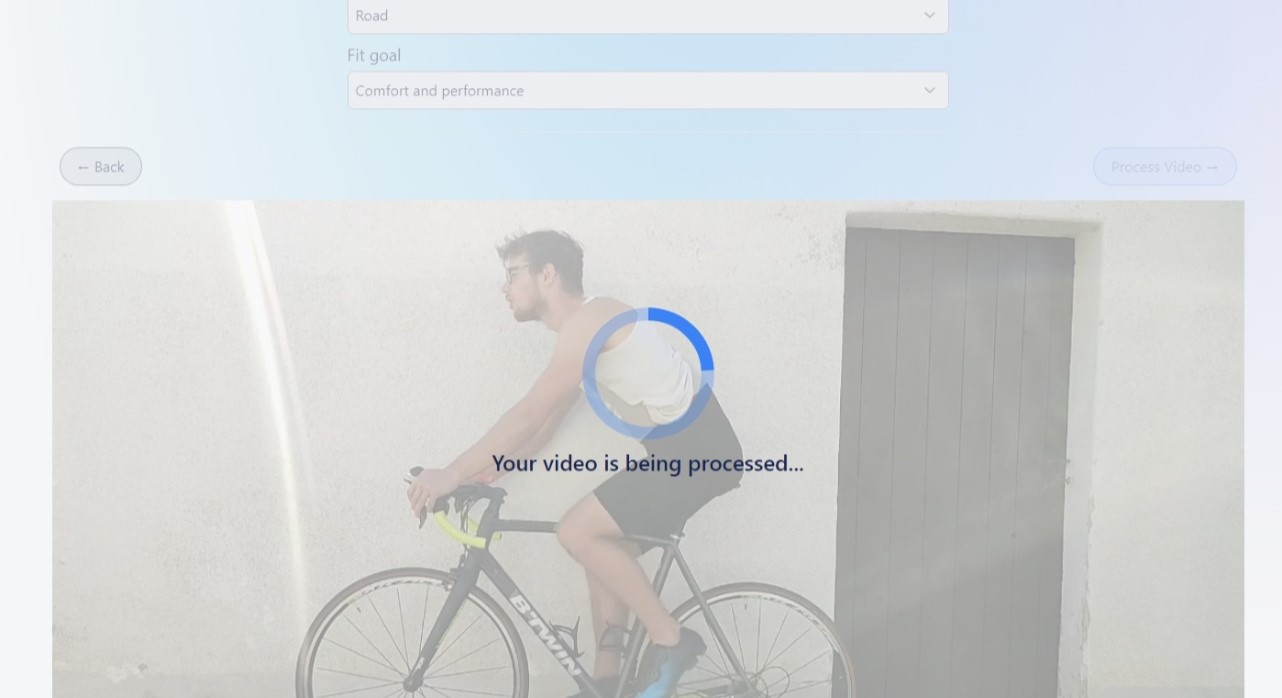
\includegraphics[width=\textwidth]{obrazky-figures/processing-crop.jpeg}
    \caption{After the user selects the fit goals, the video is processed by the pose estimation model. The user can see the progress of the processing by the progress circle in the middle of the screen.}
    \label{fig:processing}
\end{figure}


\subsection{Examine Suggestions} On the last step, after the video is processed, the user can examine the keypoint predictions from the pose estimation model, computed joint angles, suggested angle ranges and the suggestions for the bike fit. The user can also play the video with the keypoint predictions overlaid on the video. Figure \ref{fig:step3-top} shows the first part of this step. The user is presented with a video player with the keypoint predictions and measured angles overlaid on the video.


\begin{figure}[htbp]
    \centering
    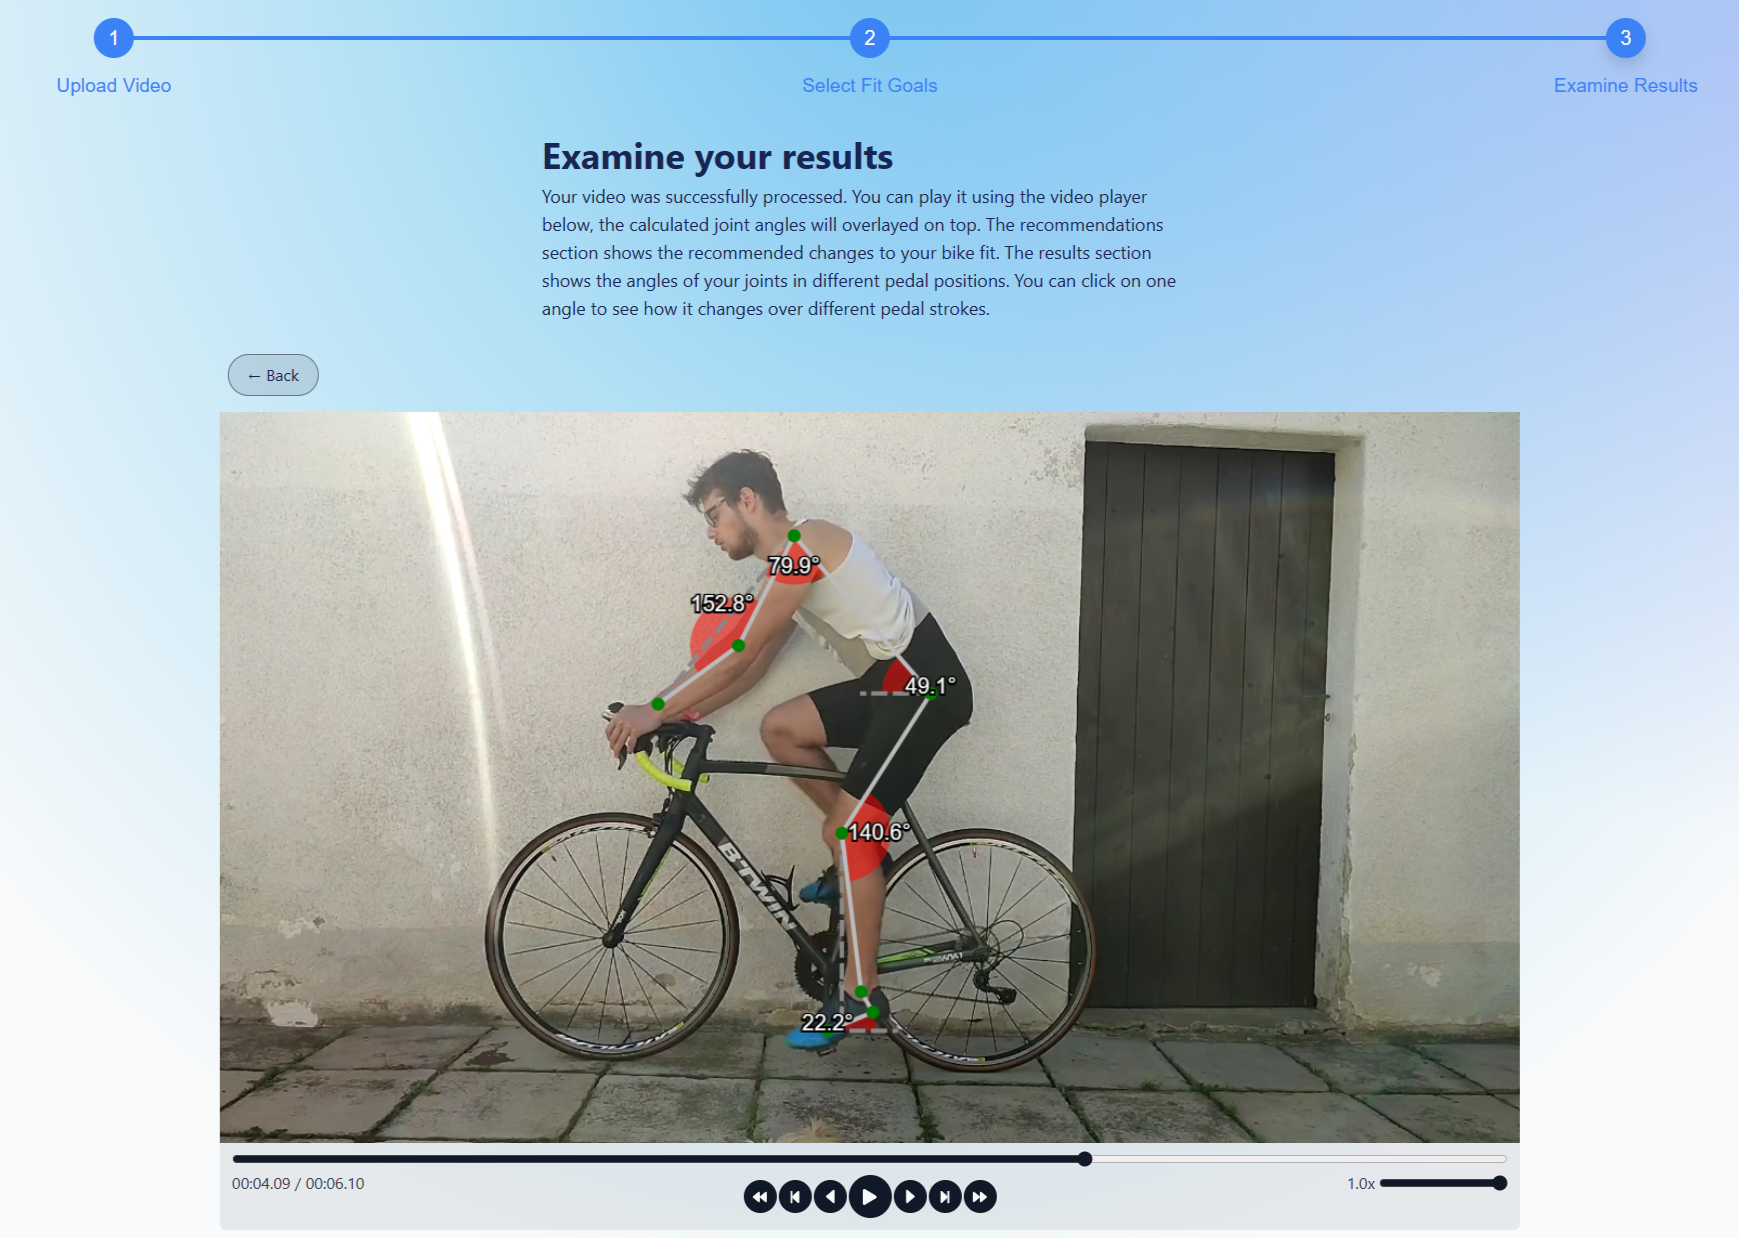
\includegraphics[width=\textwidth]{obrazky-figures/step3-top-crop.png}
    \caption{The first part of the last step of the bikefit application. The user can play the video with the keypoint predictions and measured angles overlaid on the video. For each angle, the user sees the current value and a sector of a circle connecting angle points. The video speed can be adjusted by the slider on the right. The user can also seek forward and backward 1 frame by clicking the buttons on the left and right of the middle play button. The buttons on the side can be used to seek to the next or previous pedal position and next or previous pedal stroke.}
    \label{fig:step3-top}
\end{figure}

Figure \ref{fig:step3-bottom} shows the second part of the last step of the application. The "Recommendations" section shows the bike type and fit goal selected by the user. The user can also see the assessment and suggested changes to their saddle height, saddle setback, handlebar height and handlebar reach. For each measurement, the user sees a verbal assesment of a measurement (e.g. "Too high", "Too far back", "Withing range", etc.) a graphical representation of the measurement by a colored slider input and a verbal suggestion for the change (e.g. "Lower by 1 cm", "Move saddle forward by 1 cm", etc.).

The "Results" section shows the recommended ranges and measured values for the angles and measurements in each of the pedal positions (bottom, top and front). The measurements are organized in a table-like structure, with columns for the measurement name, the measured value, a colored slider input indicating the measurement value and the recommended range. Additionally, the user can click on the visibility indicator on the left to hide or show the measurement in the video player. After clicking on a row in the table, the row expands to show more detailed information about the measurement. The user can see a chart with the angle values for each pedal stroke, with sections of the chart colored according to the recommended ranges (green for within range, yellow for close to the range and red for outside of the range). The user can also see the minimum, maximum, median and range of the measurement. In the future, additional information about the measurement and its effect on the bike fit could be added.

\begin{figure}[htbp]
    \centering
    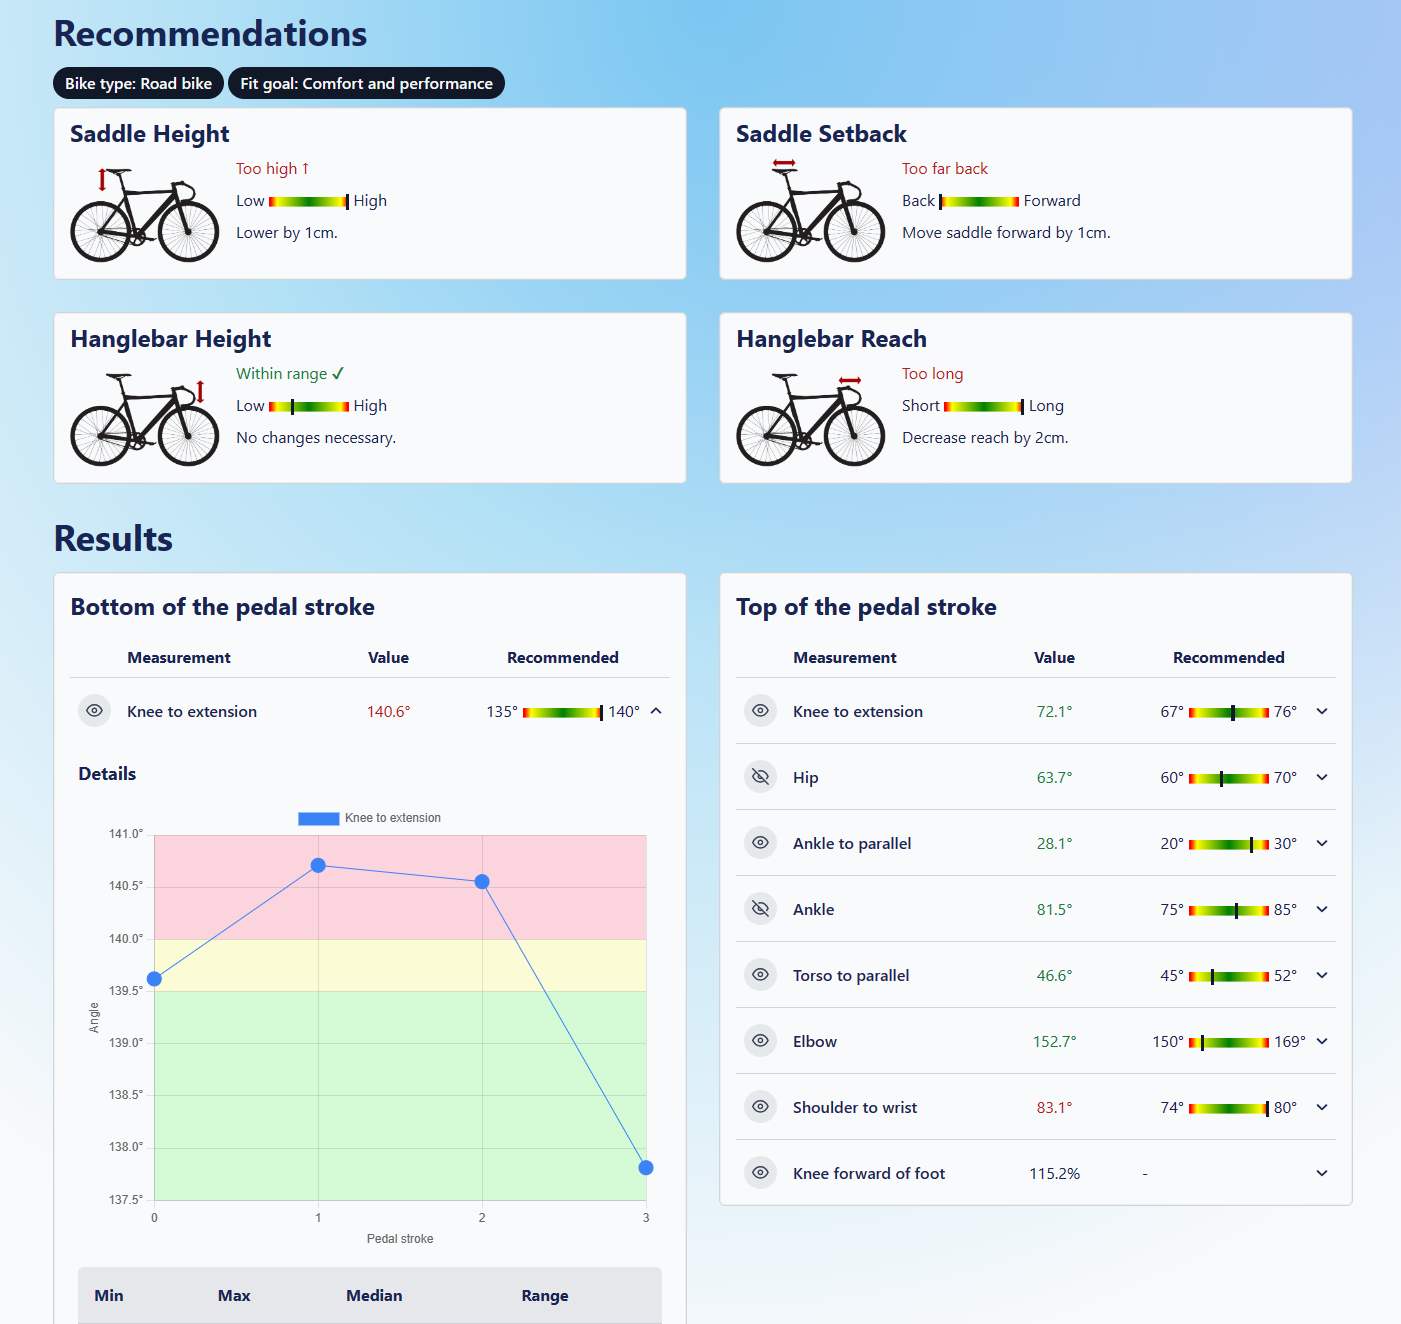
\includegraphics[width=\textwidth]{obrazky-figures/step3-bot-crop.png}
    \caption{The second part of the last step of the bikefit application. In the "Recommendations" section, the user can see the suggested changes to their saddle height, saddle setback, handlebar height and handlebar reach. In the "Results" section, the user can see the recommended ranges and measured values for the angles and measurements in each of the pedal positions (bottom, top and front (not shown)). After clicking on a measurement, the user can see a chart with the angle values for each pedal stroke, with sections of the chart colored according to the recommended ranges.}
    \label{fig:step3-bottom}
\end{figure}





\section{Video Upload and Frames Extraction}
\label{video_upload_and_processing}
At first, the video needs to be uploaded to the application. The video is uploaded using the HTML5 file input. The file is then converted to a URL using the \texttt{URL.createObjectURL()} method, because the WebCodecs API requires a URL as input.

\subsection{Accessing the Video Frames}

To accurately estimate the keypoints, the application needs to access all of the video frames and process them. This is not trivial to do in the browser. The browser does not allow the application to access the video frames directly.

To process the video frame by frame, the application uses the WebCodecs API\footnote{\url{https://developer.mozilla.org/en-US/docs/Web/API/WebCodecs_API}}. The WebCodecs API is a low-level API for encoding and decoding audio and video. It gives developers access to the invididual frames of the video. It is the only way to access the frames of the video in the browser. Simple and commonly used method is to simultaneously play the video and draw the video  frames to a canvas element and then access the pixels of the canvas. However, this method only does not work well if the processing is computationally expensive, since the video is played in real time. This leads to skipping of the frames and not all of the frames are processed. The WebCodecs API allows the application to process the video at its own pace.

Because the API is relatively new, it is not yet supported by all browsers. Figure \ref{fig:caniuseWebcodecs} shows the browser support for the WebCodecs API as of January 2024. The API is supported by all browsers based on Chromium (Google Chrome, Microsoft Edge, Opera, Brave, etc.). It is Partially supported by Safari and Safari on iOS (video only) and not supported by Firefox. Overall based on CanIUse data\footnote{\url{https://caniuse.com/webcodecs}}, the API is supported by 87.6\% of the users, where 74.5\% of the users have full support and 13.1\% of the users have partial support.


\begin{figure}[htbp]
    \centering
    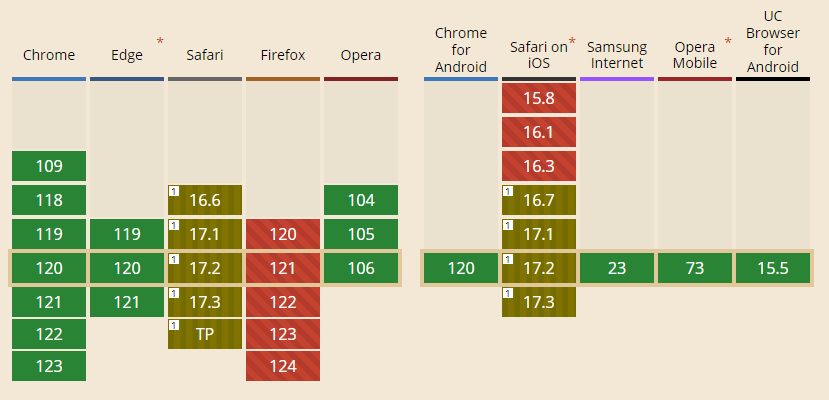
\includegraphics[width=\textwidth]{obrazky-figures/caniuseWebcodecs.png}
    \caption{Browser support as of January 2024 for the WebCodecs API. Green color indicates full support, yellow color indicates partial support and red color indicates no support. Taken from \url{https://caniuse.com/webcodecs}.}
    \label{fig:caniuseWebcodecs}
\end{figure}

Due to the low-level design of the WebCodecs API, it is not easy to use. Moreover, the API is quite new and not very well documented so there is not a lot of examples. The developer also needs to take care of demuxing the media containers. This work uses the getVideoFrames.js library\footnote{\url{https://github.com/josephrocca/getVideoFrames.js}} from josephrocca. The library internally uses the WebCodecs API and MP4Box.js\footnote{\url{https://github.com/gpac/mp4box.js/}} for demuxing mp4 files, but provides a simple interface for accessing the video frames. The library is used to get the video frames and then the frames are processed as described in sections \ref{marker_based_tracking} and \ref{pose_estimation}. It defines three callback functions. The \texttt{onFrame} callback is called for each frame of the video. The \texttt{onConfig} callback is called when the video metadata is loaded. The \texttt{onFinish} callback is called when all of the frames are processed. Overall, WebCodecs API is a powerful tool for processing video in the browser, but it relies on third party demuxing libraries and is not yet supported by all browsers.

% \begin{lstlisting}[style=htmlcssjs, caption={Example usage of the getVideoFrames.js library. Taken from \url{https://github.com/josephrocca/getVideoFrames.js/}.}, label={getVideoFrames}]
%     <canvas id="canvasEl"></canvas>
%     <br>
%     <input type="file" accept="video/mp4" onchange="start(this.files[0])">
%     <script type="module">
%       import getVideoFrames from "https://deno.land/x/get_video_frames@v0.0.10/mod.js"

%       let frameCount = 0;

%       window.start = async function(file) {
%         let ctx = canvasEl.getContext("2d"); 

%         // `getVideoFrames` requires a video URL as input.
%         // If you have a file/blob instead of a videoUrl, turn it into a URL like this:
%         let videoUrl = URL.createObjectURL(file);

%         await getVideoFrames({
%           videoUrl,
%           onFrame(frame) {  // `frame` is a VideoFrame object: https://developer.mozilla.org/en-US/docs/Web/API/VideoFrame
%             ctx.drawImage(frame, 0, 0, canvasEl.width, canvasEl.height);
%             frame.close();
%             frameCount++;
%           },
%           onConfig(config) {
%             canvasEl.width = config.codedWidth;
%             canvasEl.height = config.codedHeight;
%           },
%           onFinish() {
%             console.log("finished!");
%             console.log("frameCount", frameCount);
%           },
%         });

%         URL.revokeObjectURL(file); // revoke URL to prevent memory leak
%       }
%     </script> 
% \end{lstlisting}



\section{Pose Estimation}
\label{pose_estimation}
To get the locations of the 8 keypoints (foot, heel, ankle, knee, hip, shoulder, elbow, wrist) in the video, the RTMPose-m 256x192 Body8-Halpe26 model is used. The model is trained on the custom bike fitting dataset, as described in chapter \ref{training_pose_estimation_model_for_bikefitting}. The model is run on each frame of the video and the keypoints are extracted.

Since JavaScript is single-threaded and the model is computationally expensive, the model is run in a Web Worker. Web Worker is a JavaScript feature that allows the application to run a script in a separate thread. This allows the application to run long tasks in the background without blocking the main thread.

The keypoints are then used to compute the joint angles and generate the suggestions for the bike fit.
\subsection{Model Conversion and Deployment}
The RTMPose models are originally trained in the PyTorch framework. To run the model in the browser, the model needs to be converted to either ONNX or TensorFlow.js format. ONNX model can be run in the browser using ONNX Runtime Web \footnote{\url{https://onnxruntime.ai/docs/tutorials/web/}}. However, the ONNX Runtime Web only provides API for running the model, but does not provide tensor operations needed for preprocessing the input and postprocessing the output. Due to these reasons, TensorFlow.js is used instead.

To convert the model to TensorFlow.js format, the model is first converted to ONNX format using the MMDeploy \cite{mmdeploy} toolset. The MMDeploy toolset is a set of tools for converting models from the various OpenMMLab frameworks (MMPose, MMAction, MMDetection, etc.) to ONNX and other formats and provides an easy way to deploy the RTMPose models.

The ONNX model is then first converted to the TensorFlow SavedModel format using the unofficial onnx2tf \cite{onnx2tf} tool. The SavedModel format is a universal format for storing TensorFlow models. The SavedModel format is then converted to the TensorFlow.js format using the official TensorFlow.js converter \footnote{\url{https://github.com/tensorflow/tfjs/tree/master/tfjs-converter}} provided by the TensorFlow.js team.

The TensorFlow.js converter also quantizes the model to float16 to reduce the size of the model and speed up the inference. Quantization is a process of converting the weights and activations of the model from float32 to float16. This reduces the size of the model by half and can speed up the inference without significant loss of accuracy. The quantized model is then used in the application.

TensorFlow.js provides several different backends for running the model. The CPU backend runs the model on CPU, using JavaScript for the computation and is the slowest, but has support for all of the operations. The WebGL backend runs the model on the GPU using WebGL shaders and is the faster, but introduces very noticeable latency when the model is first run, because the WebGL API is not designed for running deep learning models and the model needs to be compiled to the shaders. The WebAssembly backend runs the model on the CPU using WebAssembly and is the faster than the CPU backend, but slower than WebGL for the larger models. The WebGPU backend runs the model on the GPU and should be the fastest, because it is designed with deep learning in mind, but is not yet supported by all browsers. From the major browsers, the WebGPU backend is only supported by Google Chrome, Microsoft Edge and Chrome on Android. This application uses the WebGPU backend if it is available, otherwise it falls back to the WebGL backend.
\subsection{Preprocessing}
The RTMPose models are a top-down pose estimation model, which means that the model requires the input image to be cropped around the person. To crop the image, the bounding box of the person is first detected using the COCO-SSD \footnote{\url{https://github.com/tensorflow/tfjs-models/tree/master/coco-ssd}} model, available in the TensorFlow.js model zoo. It is a Single Shot Detector (SSD) \cite{ssd} model trained on the COCO \cite{coco} dataset. To speed up processing the model is ran only once on the first frame of the video, because the person is assumed to be in the same position in all of the frames. The COCO-SSD is not the most accurate or the fastest model, but it is readily available in the TensorFlow.js model zoo and is good enough for using it on the first frame of the video.

The bounding box of the person is then expanded by 2.5\% on the left and right and by 20\% on the bottom to account for changing legs position of the user due to pedaling. The bounding box is then used to crop the image. The cropped image is then resized to 256x192 pixels, which is the input size of the RTMPose model and normalized by the mean and standard deviation of the Body8 dataset (mean = [123.675, 116.28, 103.53], std = [58.395, 57.12, 57.375]).

\subsection{Postprocessing}
The RTMPose models output a SimCC \cite{simcc} heatmap, which is a heatmap of the keypoints where the x and y axis are separated. This significantly reduces the number of parameters of the model and speeds up the inference. For each keypoint, the model outputs a list of scores for x and y axis. To find the location of the keypoint, the argmax of x and y axis is taken. The x and y coordinates are then divided by 2 because the models output the coordinates multiplied by 2 to increase accuracy. The x and y coordinates are then adjusted for the resizing and added to the bounding box coordinates to get the coordinates in the original image. Only 8 body keypoints on the camera facing side (foot, heel, ankle, knee, hip, shoulder, elbow, wrist) are used further, the other keypoints are discarded. The keypoints over all of the frames are then smoothed usign a Savitzky-Golay filter \cite{savgol} to reduce the noise in the predictions.

\section{Computing Joint Angles and Measurements}
\label{computing_joint_angles}

After the location of the 8 keypoints is estimated, the joint angles and measurements for the current frame are computed. Joint angles are specified either by three keypoints if the angle is computed between two bones or by two keypoint if the angle is computed between one bone and the horizontal axis.

Other than joint angles, application also computes the knee forward of foot measurement, which is the distance between the knee and the vertical line through the foot. Due to the absence of real world units in the video, the measurement is expressed as the percentage of the length from the fifth metatarsal to the heel. This measurement is used to determine saddle setback as its very similar to the widely used knee over pedal spindle (KOPS) measurement.

\subsection{Determining the Pedal Position}

For most of the measurments, the values for every frame are not in themselves very useful. For measurements that barely change over the pedal stroke (mainly upper body joint angles), the average value over all of the frames is used. For measurements that change over the pedal stroke (lower body measurements such as knee angle, knee forward of foot, ankle angle), are compared to the recommended ranges in a specific pedal position (bottom, top, front). Therefore the current pedal position needs to be determined.

To determine the pedal position for each frame, invididual pedal strokes need to be detected. To do that, a circle is fitted to the foot keypoints over all of the frames using a least squares method. This circle is then used to determine the pedal position. For example, to determine the front pedal position, the angle of the foot keypoint on the circle is computed for each frame in a pedal stroke. The front pedal position is then determined as the frame with the angle closest to 90 degrees (horizontal forward). Similarly, the bottom pedal position is determined as the frame with the angle closest to 180 degrees (vertical down) and the top pedal position is determined as the frame with the angle closest to 0 degrees or 360 degrees (vertical up). After obtaining the list of frames for each pedal position, and list of frames for each pedal stroke, we can finally compute the measurements and joint angles for each pedal position. To do this, median value of the measurements for each pedal position is used. This is done to avoid the influence of the outliers in the measurements.


\section{Generating Suggestions}
\label{generating_suggestions}
After the joint angles and measurements are computed for each pedal position, the suggestions for the bike fit are generated. The suggestions are generated based on comparing some of the measurements in the pedal positions to the recommended ranges. The recommended ranges are based on the bike fit guidelines and are then adjusted based on the type of the bike and the fit goals selected by the user. For example, saddle height recommendations are based on knee angle at the bottom of the pedal stroke. If the knee angle is inside the recommended range, saddle height is considered correct. If the knee angle at the bottom of the pedal stroke is at the lower 10 percent of the recommended range, a suggestion to increase the saddle height slightly (by 1 cm) is generated. If the knee angle is lower than the recommended range, a suggestion to increase the saddle height significantly (by 2 cm) is generated. Suggestions are made similarly when the knee angle is at the upper 10 percent of the recommended range or higher than the recommended range.

In total, suggestions are generated for the saddle height, saddle setback, handlebar height and handlebar reach. As was mentioned before, saddle height is determined by the median knee angle at the bottom of the pedal stroke. Saddle setback is determined by the median knee forward of foot measurement at the front of the pedal stroke. Handlebar height is determined by the median shoulder angle at all of the frames and handlebar reach is determined by the median shoulder angle at all of the frames.

Basing suggestions only on a single measurement is not ideal, because in reality the bike fit is a complex process and the measurements are interdependent. For example, increasing the saddle height will also increase the saddle setback, handlebar reach also influences back angle not only shoulder angle and so on. In the future, the suggestions could be generated using a more complex model, which would take into account all of the measurements and their interdependencies.
\section{Video Player}
\label{video_player}
To play the video with the predicted keypoints and measurements overlaid on the video, the application implements a custom video player based on the HTML canvas and video elements. The video is played on a hidden video element and the frames are drawn to a canvas element. This is done so that joint angles and measurements can be drawn on top of the video frames. The video player allows the user to play the video, seek to a specific time, seek to the next or previous pedal position and seek to the next or previous pedal stroke. The video player also allows the user to adjust the speed of the video.

However, there does not exist a standard way to get the index of the current frame of the video. The video element has a \texttt{currentTime} property, which returns the current time of the video in seconds, but there is no property that returns the current frame index, or even the video frames per second. Another reason why relying on the \texttt{currentTime} property is not ideal is that the \texttt{currentTime} property returns the time of the video but the video can be longer than the video track, also the video track can have variable frame rate.

This is why, to get the current frame index, the application saves the frame timestamps obtained when processing the video with the WebCodecs API. And then uses the requestVideoFrameCallback \footnote{\url{https://developer.mozilla.org/en-US/docs/Web/API/HTMLVideoElement/requestVideoFrameCallback}} to get the current frame index. The requestVideoFrameCallback is a new API that allows the application to accurately get the current video track time using the \texttt{metadata.mediaTime} property. The \texttt{metadata.mediaTime} property returns the current time of the video track in seconds. The application then finds the closest frame timestamp to the current video track time and uses the index of the frame timestamp as the current frame index. This way the application can accurately get the current frame index of the video.


%TODO: all of the types of the bike and fit goals

%%%%%%%%%%%%%%%%%%%%%%%%%%%%%%%%%%%%%%

\chapter{Web Application Experiments}
\label{experiments}

This chapter describes the experiments done to evaluate the bikefitting web application. The experiments are divided into two parts. Section \ref{assesment_of_multiple_saddle_heights} tests the application's ability to to asses and make suggestions for saddle height. Section \ref{speed_of_the_video_processing} measure how long the application takes to process one frame of the video on different devices.

\section{Testing Multiple Saddle Heights}
\label{assesment_of_multiple_saddle_heights}
To test the typical use case of the application, the application is used to set up the saddle height of a cyclist. The author filmed 6 videos of himself cycling on a road bike in a stationary trainer with various saddle heights. The saddle heights ranged from 3.5 cm lower than the usual saddle height to 2.5 cm higher than the usual saddle height. The goal of this test is to see if the measured knee angle at the bottom of the pedal stroke, which is the main measurement used to determine the saddle height, correctly increases with the saddle height and if the application recommended angles correspond to the feelings of the author about the saddle heights.

The videos were filmed outside in daylight with a resolution of 1920x1080 pixels and a frame rate of 30 frames per second using a smartphone. The author has experience riding a road bike and is modereately fit, but is not a professional cyclist. Therefore the balanced fit goal is selected for the test. The type of the bike is set to road bike. This configuration corresponds to recommended knee angle at the bottom of the pedal stroke of 135° to 140°.




Table \ref{tab:saddle_height_setup} shows the results of the test. The measured knee angle at the bottom of the pedal stroke, the recommended knee angle and the feelings of the author about the saddle height are shown for each video. The results show that the measured knee angle at the bottom of the pedal stroke increases with the saddle height, as expected. The measured knee angle is within the recommended range of 135° to 140° for the saddle heights of 0 cm -0.5 cm and -1.5 cm. This surprisingly well correspond to the feelings of the author about the saddle height. The extreme saddle heights of -3.5 cm and +2.5 cm are correctly assessed as too low and too high, respectively. The saddle height of -1.5cm felt low, but much better than the previous height of -3.5 cm, and could be used for begineers or for riders with some flexibility issues. The saddle height of -0.5 cm felt lower than the author is used to, but again, better than the previous height of -1.5 cm and could definetely be used long term. The saddle height of 0 cm felt ok and the saddle height of +0.5 cm felt distinctly too high, it was a small change, but very noticeable and the author had trouble to pedal smoothly with this saddle height.

\begin{table}[htbp]

    \centering
    \begin{tabular}{c c p{0.25\textwidth} p{0.3\textwidth}}
        \toprule
        Saddle Height & Knee Angle & Rider Feelings              & App Assesment                                             \\
        \midrule
        -3.5 cm       & 128.5°     & Too low.                    & Too low. Raise saddle by 1 cm and try again.              \\
        \midrule
        -1.5 cm       & 135.2°     & Low end of rideable window. & On lower end of range. Try raising by 5 mm and try again. \\
        \midrule
        -0.5 cm       & 137.5°     & Lower than used to, but ok. & Within range.                                             \\
        \midrule
        0 cm          & 138.8°     & Ok.                         & Within range.                                             \\
        \midrule
        +0.5 cm       & 141.3°     & Too high. Not comfortable.  & Too high. Lower saddle by 1 cm and try again.             \\
        \midrule
        +2.5 cm       & 152.3°     & Definetely too high.        & Too high. Lower saddle by 1 cm and try again.             \\
        \bottomrule
    \end{tabular}
    \caption{Results of the saddle height setup test. The measured knee angle at the bottom of the pedal stroke, the recommended knee angle and the feelings of the author about the saddle height are shown for each video.}
    \label{tab:saddle_height_setup}
\end{table}

Figure \ref{fig:saddle_height_setup} shows screenshots of the videos with saddle heights of -3.5 cm and +2.5 cm. We can see how the knee angle at the bottom of the pedal stroke changes with the saddle height. The keypoint predictions and angles are overlaid on the video.

\begin{figure}[htbp]
    \subfloat{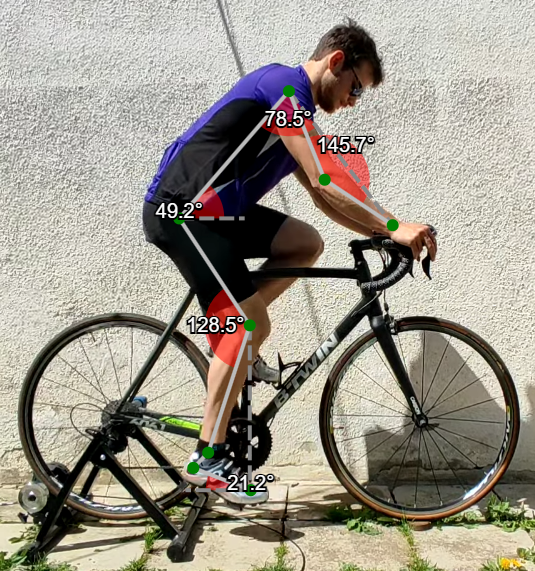
\includegraphics[width=0.49\textwidth]{obrazky-figures/-3.5_screen_crop.png}}\hfill
    \subfloat{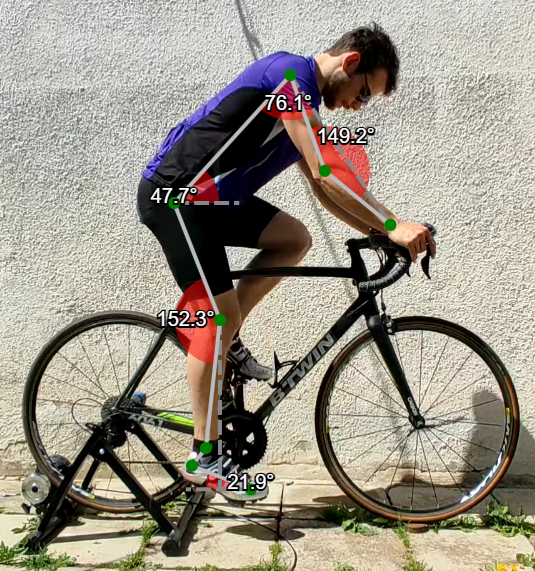
\includegraphics[width=0.49\textwidth]{obrazky-figures/+2,5_screen_crop.png}}
    \caption{Screenshots of the videos with saddle heights of -3.5 cm (left) and +2.5 cm (right) with the keypoint predictions and angles overlaid on the video. Both screenshots show the knee angle at the bottom of the pedal stroke.}
    \label{fig:saddle_height_setup}

\end{figure}

The test showed, that even small changes in the saddle height have effect on the knee angle at the bottom of the pedal stroke measured by the application. It also showed that the recommended knee angles correspond are well chosen and correspond to the feelings of the author about the saddle height. It also corresponds to bikefit literature, which states that having a slightly lower saddle height is better than having a slightly higher saddle height. The test also showed that the application can be used to set up the saddle height of a cyclist. In the future, similar tests could be done for other measurements and joint angles to further validate the application and adjust the recommended ranges.

\section{Video Processing Benchmark}
\label{speed_of_the_video_processing}
To test the speed of the pose estimation model inference and the overall processing pipeline, the time needed to process a video is measured. The benchmark is run on a desktop computer with an NVIDIA GeForce GTX 950 GPU, using Microsoft Edge browser and WebGPU backend and on a Xiaomi Redmi Note 10 Pro with Adreno 618 GPU, using Google Chrome browser and WebGL backend.

Table \ref{tab:video_processing_time} shows the time needed to process a video frame by frame on both devices. The results show that the WebGPU backend on desktop is around 2 times faster than the WebGL backend on the smartphone. Another interesting observation is on WebGPU backend, the inference time of the model is only a small part of the total frame time, while on the WebGL backend, the inference time is the majority of the total frame time. This is probably due to the fact that the WebGPU backend is more optimized for deep learning models, but has slower transfer of the data between the CPU and GPU. Another reason for long frame time on the WebGPU compared to inference time is probably not optimal implementation of the application, which could be improved in the future.

\begin{table}[htbp]
    \centering
    \begin{tabular}{l l  c c c}
        \toprule
        Device     & Backend & Inference Time & Model Time & Frame Time \\
        \midrule
        Desktop    & WebGPU  & 45-70 ms       & 85-120 ms  & 160-200 ms \\
        Smartphone & WebGL   & 220-300 ms     & 250-320ms  & 325-400 ms \\
        \bottomrule
    \end{tabular}
    \caption{Time needed to process a video frame by frame on a desktop computer with an NVIDIA GeForce GTX 950 GPU and on a Xiaomi Redmi Note 10 Pro with Adreno 618 GPU. Inference time is the time needed to run the model inference on a single frame. Model time is the time needed to run the model on a single frame, including the preprocessing and postprocessing. Frame time is the time needed to process a single frame, including the model time and time needed to decode the frame.}
    \label{tab:video_processing_time}
\end{table}


%%%%%%%%%%%%%%%%%%%%%%%%%%%%%%%%%%

\chapter{Conclusion}
\label{conclusion}

This work focused on the development of a web application for bike fitting using pose estimation. The application was successfully implemented and deployed \footnote{\url{https://vlasakjiri.github.io/bikefit/}}.

The first chapter of the work described the needed bikefitting background and existing bikefitting applications and systems and their limitations. Then the following chapters describe a marker-based method for tracking the cyclist's body and marker-less pose estimation models. Next, a custom dataset for bikefitting featuring 2309 photos of the author pedaling on a stationary trainer was created. The dataset was used to evaluate the pose estimation models and fine-tune the RTMPose model, whose Normalized Mean Error was significantly reduced from 2.54 to 1.51. Next chapter describes the implementation of the web application and the deployment process of the pose estimation model. The last chapter describes the experiments done to evaluate the application.

The resulting application, which runs fully in the browser, is able to accurately estimate the keypoint positions of the cyclist from the side view video and compute the joint angles and measurements. The application then generates suggestions for the bike fit based on the computed joint angles and recommended ranges. The application also allows more advanced users to examine the keypoint predictions and joint angles in the video player and see how the angles change over multiple pedal strokes. The experiments showed that that the application detects angle changes caused by the saddle height changes and that the application can be used to set up the saddle height. Benchmarks also showed that an older desktop computer can process a frame in 160-200 ms and a modern smartphone can process a frame in 325-400 ms.

In the future, the model accuracy could be further improved by fine-tuning it on a larger dataset, perhaps obtained by annotating the videos uploaded by the users. Using a model which also predicts hand keypoints could be used to generate suggestions based on the wrist angle. The user experience could be further improved by creating a landing page for the application, and connecting it to a database of users to store the videos and the results of the bike fit. Additionally, suggestions for fit changes could be generated by taking into account more measurements and their interdependencies.


%=========================================================================

% For compilation piecewise (see projekt.tex), it is necessary to uncomment it
% \end{document}